% !TeX encoding = UTF-8

% ###############################################################################################################################
%% Thesis Template
%% by Jörn Malzahn, Christoph Krimpmann, Christoph Rösmann, Maximilian Krämer, Mirko Waldner, Heiko Renz, Stefan Schütte
%% This template has been designed to be compliant with the requirements of the VDI Verlag-
%% See VDIVerlag-Hinweise-31_03_2013.pdf for details.
%% The basic principle of these requirements is: you submit a compliant A4 print and they will guarantee a high quality A5 book.
% ###############################################################################################################################


\documentclass[12pt,a4paper,twoside,headsepline,captions=tableheading,toc=bibliography,openany,chapterprefix]{scrbook}
% \documentclass[draft,12pt,a4paper,twoside,headsepline,captions=tableheading,toc=bibliography,openany]{scrbook} % draft version
% It uses the draft switch, which will not include the graphics in your output document. Instead it draws bounding boxes for each figure and highlights overfull boxes, and highlights exceeding margins. This is particularly usefull to hunt down overfull boxes.

%& Settings
% !TeX encoding = UTF-8

% Main settings
\usepackage{etoolbox} % Useful scripts including if/then/else
\newtoggle{lang_eng}
\newtoggle{thesis_phd}
\newtoggle{useNom}
\settoggle{lang_eng}{false} % true: english, false: german
\settoggle{thesis_phd}{false} % true: PhD, false: BT/MT
\settoggle{useNom}{false} % true: With nomenclature; false: With glossaries


%% Additional SHARED packages (WARNING: These packages also share into the tikz standalone files!)
% !TeX encoding = UTF-8


%% Font
\usepackage[utf8]{inputenc}
\usepackage[T1]{fontenc}
\usepackage{lmodern} % latin modern as main serif font for text and amth
\linespread{1.05} % TODO remove if space runs out
\usepackage[scaled=.90]{helvet} % Helvetica as font without serifs
\usepackage{courier} % Courier as type writer font
\usepackage{textcomp} % Euro symbol and many more  (use e.g. \texteuro)
\usepackage{hyphenat} % hyphenation of words

%% Language
\iftoggle{lang_eng}{\usepackage[english]{babel}}{\usepackage[ngerman]{babel}}
\usepackage[babel,autostyle]{csquotes}



%% Microtype
\usepackage[activate={true,nocompatibility},tracking=true,kerning=true,spacing=true,stretch=10,shrink=10,babel]{microtype}
% activate={true,nocompatibility} - activate protrusion and expansion
% final - enable microtype; use "draft" to disable
% tracking=true, kerning=true, spacing=true - activates these techniques
% stretch=10, shrink=10 - reduce stretchability/shrinkability (default is 20/20) 
	
	
%% Math and stuff
\usepackage{mathtools} % already loads amsmath
\usepackage{amssymb} % already loads amsfonts
\usepackage{amsthm}
\usepackage{amsfonts}
\usepackage[super]{nth} % \nth{1}, \nth{2}, \nth{3}, \nth{4}

% Define abbrev. for norms
\DeclarePairedDelimiter\abs{\lvert}{\rvert}%
\DeclarePairedDelimiter\norm{\lVert}{\rVert}%

% Swap the definition of \abs* and \norm*, so that \abs and \norm resizes the size of the brackets, and the starred version does not.
\makeatletter
\let\oldabs\abs
\def\abs{\@ifstar{\oldabs}{\oldabs*}}
%
\let\oldnorm\norm
\def\norm{\@ifstar{\oldnorm}{\oldnorm*}}
\makeatother


%% Colors
\usepackage[table,hyperref]{xcolor}
% !TeX encoding = UTF-8

%% Define user colors in RGB

% gray scale colors
\definecolor{black}{rgb}{0.0,0.0,0.0}
\definecolor{darkgray}{rgb}{0.8,0.8,0.8}
\definecolor{lightgray}{rgb}{0.95,0.95,0.95}

% rst colors
\definecolor{rstgreen}{rgb}{0.5,0.73,0.15}
\definecolor{rstorange}{rgb}{0.93,0.49,0.19}
\definecolor{rstblue}{rgb}{0.0,0.44,0.75} % Color settings
	
	
%% Useful package for SI units
\usepackage[exponent-product = \cdot,
output-complex-root = j, 
separate-uncertainty = true,
arc-separator = \,,
product-units = bracket-power]{siunitx}
\sisetup{detect-all} % detect font faces, sizes etc.
\iftoggle{lang_eng}{\sisetup{locale=US}}
{\sisetup{locale=DE}}
	

%% Figures
\usepackage{graphicx}
% Uncomment the following line to enable final mode for graphicx (show images even in draft mode)
% \setkeys{Gin}{draft=false} % disable draft mode for graphicx

\usepackage[normal,small]{caption} % Customise the captions in floating environments
\usepackage{subcaption} % split figure into subfigures
\usepackage{rotating} % sideways figures
\usepackage{pdfpages} % Include other pdf pages
	

%% Tikz
\usepackage{tikz,pgfplots}
% !TeX encoding = UTF-8

%% Tikz settings
\usetikzlibrary{automata,through,plotmarks,quotes,babel,spy,patterns,angles,positioning}
\usetikzlibrary{shapes,matrix,arrows,calc,decorations,backgrounds,intersections,fit}

% select unique fontsize (footnotesize) at the beginning of each tikz picture
\tikzset{every picture/.style={font issue=\footnotesize	},
	font issue/.style={execute at begin picture={#1\selectfont}}
}
\tikzset{fontscale/.style = {font=\footnotesize	}}

%% Pgf settings
\usepgfplotslibrary{patchplots}
\pgfplotsset{compat=newest} 
\pgfplotsset{plot coordinates/math parser=false}
\pgfplotsset{every axis plot post/.append style={line join=round}}

\iftoggle{lang_eng}{}
{
	\pgfplotsset{/pgf/number format/use comma} % Kommata für Dezimaldarstellung
	\pgfplotsset{/pgf/number format/.cd,1000 sep={}} % Trennzeichen bei 1000
}

\tikzstyle{every picture}+=[remember picture]
\tikzstyle{arrow} = [->,>=stealth']
\tikzstyle{arrowreverse} = [<-,>=stealth']
\tikzstyle{arrowbidir} = [<->,>=stealth']

% add arrow pins to axis by default
\pgfplotsset{every axis/.append style={
		axis lines = left % middle
	}
} % tikz definitions

%% Additional LOCAL packages (WARNING: These packages are NOT considered in the tikz standalone files!)
% !TeX encoding = UTF-8

%% Fixes for better KOMA support
\usepackage{scrhack} % http://tex.stackexchange.com/questions/51867/koma-warning-about-toc


%% Margins
\usepackage{geometry}	
%\usepackage[showframe]{geometry} % showframe visualizes page margins
\geometry{top=28mm,bottom=28mm,left=21mm,right=21mm,headsep=6mm,footskip=11mm,bindingoffset=8mm}


%% Misc
\usepackage{blindtext} % TODO remove later
\usepackage{enumitem} % Removes vspaces between itemize-structures with \begin{itemize}[noitemsep]...
\usepackage{twoopt} % Create commands and macros with two optional parameters TODO check if needed
\usepackage{comment} % Conditionally build comments and contents
\usepackage{standalone} % modern way of externalizing tikz
	
	
%% Theoremstyle
\newtheoremstyle{myTheoremStyle}% name
{11pt}      % Space above
{11pt}      % Space below
{\itshape}  % Body font
{}          % Indent amount (empty = no indent, \parindent = para indent)
{\bfseries} % Thm head font
{:}         % Punctuation after thm head
{.5em}      % Space after thm head: " " = normal interword space;{\newline = linebreak}
{}          % Thm head spec (can be left empty, meaning 'normal')
% !TeX encoding = UTF-8
\theoremstyle{myTheoremStyle}

\newtheorem{acknowledgement}{\iftoggle{lang_eng}{Acknowledgement}{Danksagung}}
\newtheorem{assumption}{\iftoggle{lang_eng}{Assumption}{Annahme}}[section]
\newtheorem{assumptions}{\iftoggle{lang_eng}{Assumptions}{Annahmen}}[section]
\newtheorem{axiom}{Axiom}[section]
\newtheorem{case}{\iftoggle{lang_eng}{Case}{Fall}}[section]
\newtheorem{claim}{\iftoggle{lang_eng}{Claim}{Forderung}}[section]
\newtheorem{conclusion}{\iftoggle{lang_eng}{Conclusion}{Schlussfolgerung}}[section]
\newtheorem{condition}{\iftoggle{lang_eng}{Condition}{Bedingung}}[section]
\newtheorem{conjecture}{\iftoggle{lang_eng}{Conjecture}{Vermutung}}[section]
\newtheorem{convention}{\iftoggle{lang_eng}{Convention}{Konvention}}[section]
\newtheorem{corollary}{\iftoggle{lang_eng}{Corollary}{Korollar}}[section]
\newtheorem{criterion}{\iftoggle{lang_eng}{Criterion}{Kriterium}}[section]
\newtheorem{definition}{Definition}[section]
\newtheorem{example}{\iftoggle{lang_eng}{Example}{Beispiel}}[section]
\newtheorem{exercise}{\iftoggle{lang_eng}{Exercise}{Aufgabe}}[section]
\newtheorem{lemma}{Lemma}[section]
\newtheorem{notation}{\iftoggle{lang_eng}{Notation}{Bezeichnung}}[section]
\newtheorem{problem}{Problem}[section]
\newtheorem{proposition}{\iftoggle{lang_eng}{Proposition}{Satz}}[section]
\newtheorem{remark}{\iftoggle{lang_eng}{Remark}{Bemerkung}}[section]
\newtheorem{solution}{\iftoggle{lang_eng}{Solution}{Lösung}}[section]
\newtheorem{theorem}{Theorem}[section] % define custom theorem headings
	
	
%% Tables
\usepackage{tabularx}
\usepackage{booktabs}
\usepackage{multirow}

%% Algorithm
\usepackage[section]{algorithm} % float wrapper for algorithms. Repeat counter on each section
\usepackage{algorithmicx} % actual algorithm environment
\usepackage[noend]{algpseudocode} % command set for pseudocode. noend omits all end statements
\newcommand*\Let[2]{\State #1 $\gets$ #2}

% Commands
\iftoggle{lang_eng} {}
{ 
	\algrenewcommand\algorithmicrequire{\textbf{Voraussetzung:}}
	\algrenewcommand\algorithmicensure{\textbf{Abschlussbedingung:}}
}
\algnewcommand{\algorithmicand}{\textbf{ and }}
\algnewcommand{\algorithmicor}{\textbf{ or }}
\algnewcommand{\algorithmicbreak}{\textbf{break}}
\algnewcommand{\OR}{\algorithmicor}
\algnewcommand{\AND}{\algorithmicand}
\algnewcommand{\BREAK}{\State \algorithmicbreak}

% Setup captions for algorithm
\DeclareCaptionLabelFormat{algo_format}{#1 #2.}
\captionsetup[algorithm]{name=\iftoggle{lang_eng}{Algorithm}{Algorithmus}, labelformat=algo_format,font=small,labelfont=small, labelsep=colon,justification=centering}


%% Nomenclature
\usepackage[noprefix,intoc,\iftoggle{lang_eng}{english}{german}]{nomencl}
\setlength{\nomlabelwidth}{.25\hsize}
\setlength{\nomitemsep}{-\parsep}

% Split nomenclature for symbols and abbreviations
\renewcommand{\nomgroup}[1]{%
	\ifstrequal{#1}{C}{\vspace{3mm}\item[\textbf{\iftoggle{lang_eng}{Roman symbols}{Lateinische Symbole}}]}{
		\ifstrequal{#1}{B}{\vspace{3mm}\item[\textbf{\iftoggle{lang_eng}{Greek symbols}{Griechische Symbole}}]}}{
		\ifstrequal{#1}{A}{\vspace{3mm}\item[\textbf{\iftoggle{lang_eng}{Abbreviations and Acronyms}{Abkürzungen und Akronyme}}]}{}}} 

\makenomenclature %Generates a .nlo file

% Postprocessor settings: run makeindex.exe with argument list: %tm.nlo -s nomencl.ist -o %tm.nls (TeXnicCenter -> Ausgabeprofile)
% Use \printnomenclature to create a nomenclature in your document
% Use \nomenclature[A]{abrev.}{description} for abbreviations
% Use \nomenclature[1symbol]{symbol}{description} for greek symbols
% Use \nomenclature[3symbol]{\symbol}{description} for greek symbols. Note: Rewriting the symbol name without the backslash is important for correct alpha numeric ordering! This is particularly visible if you have hats, tilde, dots, bars or anything like that to modify your greek letter.

% TexStudio:
% 1. Step: configure Makeindex 
%  Compile flags: Makeindex: makeindex.exe %.nlo -s nomencl.ist -o %.nls 
% 2. Step: run Makeindex during compilation
%  TexStudio: Tab Create: Default compiler: add makeindex (click on screwdriver button)


%% Bibliography using Biblatex
% Simple bibtex is outdated. Biblatex provides a whole lot of nice features.

\iftoggle{thesis_phd}{%
\usepackage[autolang=hyphen,style=alphabetic,giveninits=true,uniquename=allfull,isbn=false,doi=false,backend=biber,maxalphanames=2, maxnames=10,minnames=1,maxbibnames=99,defernumbers=true]{biblatex}
}{%
\usepackage[autolang=hyphen,style=authoryear-comp,giveninits=true,uniquename=init,isbn=false,doi=false,dashed=false,backend=biber,maxnames=3,minnames=1,maxbibnames=99]{biblatex}}
% Detailed information: ftp://ftp.mpi-sb.mpg.de/pub/tex/mirror/ftp.dante.de/pub/tex/macros/latex/contrib/biblatex/doc/biblatex.pdf

% Remove publisher and editor except for books
\AtEveryBibitem{	
	\ifentrytype{book}{}{%
		\clearlist{publisher}
		\clearname{editor}
	}
}

% Remove location and address
\DeclareSourcemap{
	\maps[datatype=bibtex, overwrite]{
		\map{
			\step[fieldset=address, null]
			\step[fieldset=location, null]
		}
	}
}

% We define our own bib environment in order to omit the bib key index.
\defbibenvironment{pubenv}
{\list
	{}
	{\setlength{\leftmargin}{\bibhang}%
		%\setlength{\itemindent}{-\leftmargin}%
		\setlength{\itemsep}{\bibitemsep}%
		\setlength{\parsep}{\bibparsep}}}
{\endlist}
{\item}

% Bibliography with own publications related to the thesis
\DeclareBibliographyCategory{pub}
\defbibheading{pub}[\iftoggle{lang_eng}{Related Peer-Reviewd Publications}{Relevante wissenschaftliche Publikationen}]{
	\pagestyle{myheadings}%
	\markboth{#1}{#1}%
	\section*{#1}}
	
% Bibliography for CO publications related to the thesis
\DeclareBibliographyCategory{pubco}
\defbibheading{pubco}[\iftoggle{lang_eng}{Related Peer-Reviewd Publications with Co-Authorship}{Relevante wissenschaftliche Publikationen mit Co-Autorenschaft}]{
	\pagestyle{myheadings}%
	\markboth{#1}{#1}%
	\section*{#1}}


% Bibliography for own publications NOT related to the thesis
\DeclareBibliographyCategory{pubother}
\defbibheading{pubother}[\iftoggle{lang_eng}{Additional Peer-Reviewd Publications}{Weitere wissenschaftliche Publikationen}]{
	\pagestyle{myheadings}%
	\markboth{#1}{#1}%
	\section*{#1}}
	
% Bibliography for CO publications NOT related to the thesis
\DeclareBibliographyCategory{pubotherco}
\defbibheading{pubotherco}[\iftoggle{lang_eng}{Additional Peer-Reviewd Publications with Co-Authorship}{Weitere wissenschaftliche Publikationen mit Co-Autorenschaft}]{
	\pagestyle{myheadings}%
	\markboth{#1}{#1}%
	\section*{#1}}

% Bibliography for supervised theses
\DeclareBibliographyCategory{thes}
\defbibheading{thes}[\iftoggle{lang_eng}{Supervised Theses}{Betreute Abschlussarbeiten}]{
	\newpage
	\pagestyle{myheadings}%
	\markboth{#1}{#1}%
	\section*{#1}}

% Bibliography for project groups
\DeclareBibliographyCategory{pgs}	 
\defbibheading{pgs}[\iftoggle{lang_eng}{Supervised Student Project Groups}{Betreute studentische Projektgruppen}]{
	\newpage
	\pagestyle{myheadings}%
	\markboth{#1}{#1}%
	\section*{#1}}

% Bibliography for patens
\DeclareBibliographyCategory{pat}
\defbibheading{pat}[\iftoggle{lang_eng}{Patent Applications}{Patente}]{
	\newpage
	\pagestyle{myheadings}%
	\markboth{#1}{#1}%
	\section*{#1}}

% Bibliography for your published media
\DeclareBibliographyCategory{media}
\defbibheading{media}[\iftoggle{lang_eng}{Published Software and Media}{Veröffentlichte Software und Medien}]{
	\newpage
	\pagestyle{myheadings}%
	\markboth{#1}{#1}%
	\section*{#1}}

% Make bold labels in bibliography
\usepackage{xpatch}
\xpretobibmacro{author}{\mkbibbold\bgroup}{}{}
\xapptobibmacro{author}{\egroup}{}{}
\renewcommand*{\labelnamepunct}{\mkbibbold{\addcolon\space}}

% Increase spacing between two bib items
\setlength{\bibitemsep}{0.5\baselineskip}


%% Hyperlinks, has to be the last package!
%\usepackage[colorlinks=true,urlcolor=blue,citecolor=blue,linkcolor=black]{hyperref} % for PDF
\usepackage[colorlinks=false,hidelinks,pdfpagelayout=TwoPageRight]{hyperref} % for printing
\PassOptionsToPackage{hyphens}{url}

%% Self-defined hyphenations
% !TeX encoding = UTF-8

% Just continue this space separated list
\hyphenation{Tech-ni-sche Uni-ver-si-tät Dort-mund}

%% Self-defined commands
% !TeX encoding = UTF-8

%% Define your custom commands in this file

%% New 'cite' commands to add with/without citing
\newcommand*{\citepub}[1]{\addtocategory{pub}{#1}\cite{#1}}
\newcommand*{\textcitepub}[1]{\addtocategory{pub}{#1}\textcite{#1}}
\newcommand*{\addpub}[1]{\addtocategory{pub}{#1}\nocite{#1}}

\newcommand*{\citepubco}[1]{\addtocategory{pubco}{#1}\cite{#1}}
\newcommand*{\textcitepubco}[1]{\addtocategory{pubco}{#1}\textcite{#1}}
\newcommand*{\addpubco}[1]{\addtocategory{pubco}{#1}\nocite{#1}}

\newcommand*{\citepubother}[1]{\addtocategory{pubother}{#1}\cite{#1}}
\newcommand*{\textcitepubother}[1]{\addtocategory{pubother}{#1}\textcite{#1}}
\newcommand*{\addpubother}[1]{\addtocategory{pubother}{#1}\nocite{#1}}

\newcommand*{\citepubotherco}[1]{\addtocategory{pubotherco}{#1}\cite{#1}}
\newcommand*{\textcitepubotherco}[1]{\addtocategory{pubotherco}{#1}\textcite{#1}}
\newcommand*{\addpubotherco}[1]{\addtocategory{pubotherco}{#1}\nocite{#1}}

\newcommand*{\citepat}[1]{\addtocategory{pat}{#1}\cite{#1}}
\newcommand*{\textcitepat}[1]{\addtocategory{pat}{#1}\textcite{#1}}
\newcommand*{\addpat}[1]{\addtocategory{pat}{#1}\nocite{#1}}

\newcommand*{\addpg}[1]{\addtocategory{pgs}{#1}\nocite{#1}}
\newcommand*{\addthesis}[1]{\addtocategory{thes}{#1}\nocite{#1}}
\newcommand*{\addmedia}[1]{\addtocategory{media}{#1}\nocite{#1}}

%% Math
\DeclareMathOperator{\T}{T} % Transposition T
\newcommand{\sign}[1]{\operatorname{sign}\left(#1\right)} % sign()
\newcommand*{\mtext}[1]{\text{\normalfont #1}} % enforce non-italic also in theorem environments
\newcommand{\fundef}[3]{#1\,{:}\,\mathbb{R}^{#2}\,{\mapsto}\,\mathbb{R}^{#3}}

%% Command to query document font size
\makeatletter
\newcommand\thefontsize{\f@size pt}
\makeatother

%% Misc settings
\setlength{\parindent}{0cm} % Disable automatic parindent
\setcounter{tocdepth}{2}% Allow only \chapter in ToC
\numberwithin{equation}{section} % adds section counter to equation number and resets it for every new section to match with theorem numbering. Do not use numbered equations between chapter and first section (i.e. section 0)

% Bibliography
\addbibresource{thesis.bib} % Bibtex file for main references
\iftoggle{thesis_phd}{%
\addbibresource{pub.bib} % Bibtex file for published papers (main/co-author, related/non-related)
\addbibresource{other.bib}} % Bibtex file for other own stuff (supervised theses, project groups,...)

% Customized chapter headings. We require chapterprefix for 2-line-heading but we rewrite \chapterformat to ignore the prefix
\setkomafont{chapter}{\bfseries\Huge}
\renewcommand*{\raggedchapter}{\raggedleft}
\renewcommand*{\chapterformat}{%
	\fontsize{100pt}{80pt}\selectfont\thechapter
	\vspace{-0.7ex} % adjust horizontal separation between label and title body 
}
\RedeclareSectionCommand[beforeskip=1.8ex,afterskip=1.8cm]{chapter}

%% include or exclude comments of different chapters
%\includecomment{chA/comment}
%\includecomment{chB/comment}
%\includecomment{chC/comment} % look in here for settings like languange, etc.


% ##########################################################################
% BODY
% ##########################################################################

\begin{document}
	
%% Uncomment the following three lines to display the page layout.
%\printinunitsof{cm}
%\currentpage
%\pagedesign


% ##########################################################################
% PREFACE AND INDEXES
% ##########################################################################

%% Page numbering for title, abstract, dedication and acknowledgements
% Table of contents has roman page numbering. See VDIVerlag-Hinweise-31_03_2013.pdf for details.
\pagenumbering{alph}
\pagestyle{empty} 
\let\chapterpagestyleorig\chapterpagestyle % save pagestyle for new chapters
\renewcommand*{\chapterpagestyle}{empty} % no page numbering for chapter pages

%% Title page
\iftoggle{thesis_phd}{%
\iftoggle{lang_eng}
	{% !TeX encoding = UTF-8
\makeatletter  % Do not delete this line

\title{\LARGE Title\\ %Dingsbums\\
	\vspace{2.2cm}
	{\normalsize\normalfont{A thesis approved for the academic degree of}\\
		\vspace{1.5cm}
		\normalfont{Doktor der Ingenieurswissenschaften (Dr.-Ing.)}\\
		\vspace{1.5cm}
		\normalfont{at the}\\
		\vspace{1.5cm}
		\normalfont{Faculty of Electrical Engeneering and Information Technology}\\
		\vspace{0.4cm}
		\normalfont{TU Dortmund University}\\
		\vspace{1.0cm}
		\normalfont{by}\\
		\author{\normalsize{\normalfont{Name Name, M.Sc.}}\\ \normalsize{\normalfont{Place of Birth}}}
}}

\date{\vspace{2.9cm}
	\raggedright{
		\normalsize
		\normalfont{Supervisor: Univ.-Prof. Dr.-Ing. Prof. h.c. Dr. h.c. Torsten Bertram}\\
		\normalfont{Co-Advisor: *WANTED* }\\
		\vspace{0.8cm}
		\normalfont{Day of Oral Examination: \today }\\
}}

\makeatother  % Do not delete this line
}
	{% !TeX encoding = UTF-8
\makeatletter  % Do not delete this line

\title{\LARGE Titel\\ %Dingsbums\\
	\vspace{1.7cm}
	{\normalsize\normalfont{von der}\\
		\vspace{0.4cm}
		\normalfont{Fakultät für Elektrotechnik und Informationstechnik}\\
		\normalfont{der}\\
		\normalfont{Technischen Universität Dortmund}\\
		\vspace{0.4cm}
		\normalfont{genehmigte}\\
		\vspace{1.7cm}
		\normalfont{\textbf{DISSERTATION}}\\ 
		\vspace{2.4cm}
		\normalfont{zur Erlangung des akademischen Grades}\\
		\normalfont{Doktor der Ingenieurswissenschaften (Dr.-Ing.)}\\
		\vspace{1.7cm}
		\normalfont{vorgelegt von}\\
		\vspace{1cm}
		\author{\normalsize{\normalfont{Name Name, M.Sc. }}\\ \normalsize{\normalfont{aus Ort}}}
}}

\date{\vspace{1.7cm}
	\raggedright{
		\normalsize
		\normalfont{Referent: Univ.-Prof. Dr.-Ing. Prof. h.c. Dr. h.c. Torsten Bertram}\\
		\normalfont{Korreferent: *WANTED* }\\
		\vspace{0.8cm}
		\normalfont{Tag der mündlichen Prüfung: \today }\\ 
}}

\makeatother  % Do not delete this line
}
}{%
\iftoggle{lang_eng}
	{% !TeX encoding = UTF-8
\makeatletter  % Do not delete this line


\title{
\begin{table}[t]
	\begin{tabular}{p{0.775\columnwidth} r} % 0.775 was 0.85 -> needs a proper fix!
		
\includegraphics[width=9cm]{images/logos/tud_logo_rgb} & 
\includegraphics[width=2.5cm]{images/logos/rst_logo_rgb}
	\end{tabular}
\end{table}
\LARGE Impact of Varying Collision Avoidance Strategies on Human Stress Level in Human-Robot Interaction\\ 
\vspace{0.5cm}
%\large{Subtitle (optional) }\\
\vspace{2cm}
{\normalfont\large{{\textbf{Master Thesis }}}\\ 
\vspace{1cm}
\normalfont{submitted to}\\
\vspace{1cm}
\normalfont{Institute of Control Theory and Systems Engineering}\\
\vspace{0.5cm} 
%\normalfont{der}\\
\normalfont{Faculty of  Electrical Engineering and Information Technology}\\ 
%\normalfont{der}\\
\vspace{0.5cm} 
\normalfont{Technische Universität Dortmund}\\
\vspace{1cm}
\normalfont{by}\\ 
\vspace{-1cm}
}}
\author{\normalsize{\normalfont{ Mohammed Faizan }}\\ 
\normalsize{\normalfont{Chennai, India}}}
\date{\vspace{2cm}
\raggedright{
\normalsize{\normalfont{Date of Submission: \today }\\ 
\vspace{0.5cm}
\normalfont{\textit{Responsible Professor}: }\\
\normalfont{Univ.-Prof. Dr.-Ing. Prof. h.c. Dr. h.c. Torsten Bertram}\\
\vspace{0.25cm}
\normalfont{\textit{Academic Supervisors}:}\\ 
\normalfont{M.Sc. Heiko Renz}\\
\normalfont{M.Sc. Khazar Dargahi Nobari}\\
}}
}

\makeatother  % Do not delete this line
}
	{% !TeX encoding = UTF-8
\makeatletter  % Do not delete this line


\title{
\begin{table}[t]
	\begin{tabular}{p{0.775\columnwidth} r} % 0.775 was 0.85 -> needs a proper fix!
		
\includegraphics[width=9cm]{images/logos/tud_logo_rgb} & 
\includegraphics[width=2.5cm]{images/logos/rst_logo_rgb}
	\end{tabular}
\end{table}
\LARGE Titel meiner Abschlussarbeit\\ 
\vspace{0.5cm}
\large{Untertitel (optional) }\\
\vspace{2cm}
{\normalfont\large{{\textbf{Masterarbeit / Bachelorarbeit}}}\\ 
\vspace{1cm}
\normalfont{eingereicht am}\\
\vspace{1cm}
\normalfont{Lehrstuhl für Regelungssystemtechnik}\\
\vspace{0.5cm} 
%\normalfont{der}\\
\normalfont{Fakultät für Elektrotechnik und Informationstechnik}\\ 
%\normalfont{der}\\
\vspace{0.5cm} 
\normalfont{Technische Universität Dortmund}\\
\vspace{1cm}
\normalfont{von}\\ 
\vspace{-1cm}
}}
\author{\normalsize{\normalfont{ Jane Doe }}\\ 
\normalsize{\normalfont{Geburtsort, Geburtsland}}}
\date{\vspace{2cm}
\raggedright{
\normalsize{\normalfont{Abgabedatum: \today }\\ 
\vspace{0.5cm}
\normalfont{\textit{Verantwortlicher Hochschullehrer}: }\\
\normalfont{Univ.-Prof. Dr.-Ing. Prof. h.c. Dr. h.c. Torsten Bertram}\\
\vspace{0.25cm}
\normalfont{\textit{Wissenschaftliche Betreuer}:}\\ 
\normalfont{Dipl.-Ing. Max Mustermann}\\
\normalfont{M.Sc. Lisa Müller}\\
}}
}

\makeatother  % Do not delete this line
}
}
\maketitle

%% dedication
% !TeX encoding = UTF-8

\thispagestyle{empty}
\vspace*{\fill}

\begin{center}
\begin{quote}
\enquote{\textit{Das ist die Widmung / This is the dedication (optional)}}
\end{quote}
\end{center}

\vspace*{\fill}

\cleardoublepage % force next part to start on the right page

%% acknowledgement
% !TeX encoding = UTF-8

\chapter*{\iftoggle{lang_eng}{Acknowledgement}{Danksagung}}

Das ist die Danksagung / This is the acknowledgement (optional)

\cleardoublepage % force next part to start on the right page

%% abstract
% !TeX encoding = UTF-8

\chapter*{\iftoggle{lang_eng}{Abstract}{Kurzfassung}}

The integration of collaborative robots into shared workspaces with humans has become a pivotal aspect of modern manufacturing processes, heralding a new era of human-robot interaction. This thesis addresses the human element in these interactions by investigating the impact of varying robot collision avoidance strategies on human stress levels. A series of subject study were conducted to collect physiological, motion capture, and subjective data, which were then used to analyze the perceived stress levels of participants engaged in tasks with collaborative robots across various scenarios. Different collision avoidance strategies were implemented to study their impact on human stress levels.
Another key aspect of the research was the development of a stress prediction model. This model, trained on the data collected thought the subject study, utilizing various preprocessing and feature engineering techniques. Machine learning models, including K-Nearest Neighbors, Support Vector Machines and Random Forest, among others were evaluated to identify the most effective approach for predicting stress levels. Notably, Random Forest and Support Vector Machines achieved the highest accuracy of 94\% and 91.6\% respectively.
In summary, this thesis explores the relationship between the robot collision avoidance strategies to human stress levels, providing valuable insights for designing more intuitive and stress-reducing human robot collaborative environments.
\cleardoublepage % force next part to start on the right page
  

% ##########################################################################
% MAIN CONTENTS
% ##########################################################################

% There is no list of figrues and list of tables in the template. See VDIVerlag-Hinweise-31_03_2013.pdf for details.
\setcounter{page}{1}
\pagestyle{headings} 
\pagenumbering{roman}
\renewcommand*{\chapterpagestyle}{\chapterpagestyleorig} % restore chapter pagestyle for the main content
\tableofcontents
\newpage

%% nomenclature
\iftoggle{useNom}{
% !TeX encoding = UTF-8
%%%%%%%%%%%%%%%%%%%%%%%%%%%%%%%% Nomenclature %%%%%%%%%%%%%%%%%%%%%%%%%%%%%%%%%%%
%See: http://blog.stefan-macke.com/2006/05/03/abkurzungsverzeichnis-mit-latex/

% Page style
\markboth{\nomname}{\nomname}% maybe with \MakeUppercase
\iftoggle{lang_eng}{}{\renewcommand{\nomname}{Nomenklatur}} % use german name


\printnomenclature[4cm] % There is a bug TeXnicCenter version 2.0 Beta 1. As soon as this line is added to the document the structure pane indicates a missing paragraph. Nevertheless the nomenclature package works correctly. 

%% You may remove the \iftoggle{lang_eng}{english}{german} in your version!

%% General variables
\nomenclature{$\mathbf{x}(t)$}{\iftoggle{lang_eng}{State vector at time}{Zustandsvektor zum Zeitpunkt} $t$}%
\nomenclature{$u(t)$}{\iftoggle{lang_eng}{Control input at time}{Eingangssignal zum Zeitpunkt} $t$}%
\nomenclature{$t$}{\iftoggle{lang_eng}{Time}{Zeit}}
\nomenclature{$x,y,z$}{\iftoggle{lang_eng}{Spatial coordinates}{Kartesische Koordinaten}}

%% Abkürzungen
\nomenclature[A]{Abrev.}{Abbreviation}
\nomenclature[A]{KF}{\textbf{K}alman \textbf{F}ilter}

\nomenclature[B]{$\alpha$}{\iftoggle{lang_eng}{Greek symbol}{Griechischer Buchstabe}}
}{
% SYMBOLS -----------------------------------------------------------
\newglossaryentry{xt}{name={\ensuremath{\mathbf{x}(\gls{t})}},
	description={\iftoggle{lang_eng}{State vector at time}{Zustandsvektor zum Zeitpunkt} \gls{t}},sort=1_xt
}
\newglossaryentry{xb}{name={\ensuremath{\mathbf{x}}},
	description={\iftoggle{lang_eng}{State vector}{Zustandsvektor} \gls{t}},sort=1_xt % add 1_ to sort it in the beginning since it is bold
}
\newglossaryentry{ut}{name={\ensuremath{{u}(\gls{t})}},
	description={\iftoggle{lang_eng}{Control input at time}{Eingangssignal zum Zeitpunkt} \gls{t}},sort=ut
}
\newglossaryentry{t}{name={\ensuremath{t}},
	description={\iftoggle{lang_eng}{Time}{Zeit}},sort=t
}
\newglossaryentry{xyz}{name={\ensuremath{x,y,z}},
	description={\iftoggle{lang_eng}{Spatial coordinates}{Kartesische Koordinaten}},sort=xyz
}
% Grichische Buch -----------------------------------------------------------
\newglossaryentry{alph}
{	name={\ensuremath{\alpha}},
	description={\iftoggle{lang_eng}{Greek letter}{Griechischer Buchstabe}},	sort=alpha,type = greek
}

% Abkürzungen -----------------------------------------------------------
\newacronym{mpc}{MPC}{\underline{M}odel \underline{P}redictive \underline{C}ontrol}
\newacronym{abbrev}{Abrev.}{\iftoggle{lang_eng}{Abbreviation}{Abkürzung}}
\newacronym{KF}{KF}{\underline{K}alman \underline{F}ilter}
\newacronym{GSR}{GSR}{ Galvanic Skin Response}
\newacronym{BVP}{BVP}{ Blood Volume Pulse}
\newacronym{EDA}{EDA}{ Electrodermal Activity}
\newacronym{NASA-TLX}{NASA-TLX}{National Aeronautics Space Administration–Task Load Index}
\newacronym{HR}{HR}{Heart Rate}
\newacronym{PPG}{PPG}{Photoplethysmography}
\newacronym{HRV}{HRV}{Heart Rate Variability}
\newacronym{SAM}{SAM}{Self-Assessment Manikin}
\newacronym{GAToR}{GAToR}{General Attitudes Towards Robots Scale}
\newacronym{Cobots}{Cobots}{Collaborative Robots}
\newacronym{KNN}{KNN}{K-Nearest Neighbors}
\newacronym{SVM}{SVM}{Support Vector Machines }
\newacronym{PSS}{PSS}{Perceived Stress Scale }
\newacronym{MPC}{MPC}{Model Predictive Control}
\newacronym{GMM}{GMM}{Gaussian Mixture Model }
\newacronym{TSST}{TSST}{Trier Social Stress Test}
\newacronym{NA-SW}{NA-SW}{No Collision Avoidance in a Separated Workspace}
\newacronym{NA-SHW}{NA-SHW}{No Collision Avoidance in a Shared Workspace}
\newacronym{DA-SHW}{DA-SHW}{Dynamic Collision Avoidance in a Shared Workspace}
\newacronym{PA-SHW}{PA-SHW}{Predictive Collision Avoidance in a Shared Workspace}
\newacronym{NA-DCW}{NA-DCW}{No Collision Avoidance with  Direct Collaboration in a Shared Workspace}
\newacronym{DA-DCW}{DA-DCW}{Dynamic Collision Avoidance with  Direct Collaboration in a Shared Workspace}
\newacronym{PA-DCW}{PA-DCW}{Predictive Collision Avoidance with  Direct Collaboration in a Shared Workspace}
\newacronym{IoT}{IoT}{Internet of Things}
\newacronym{TICS}{TICS}{Trier Inventory for the Assessment of Chronic Stress}
\newacronym{DSI}{DSI}{Daily Stress Inventory}
\newacronym{ST}{ST}{Skin Temperature}
\newacronym{IBI}{IBI}{Interbeat Interval}
\newacronym{SCL}{SCL}{Skin Conductance Level}
\newacronym{SCR}{SCR}{Skin Conductance Response}
\newacronym{VPG}{VPG}{Velocity Plethysmogram}
\newacronym{APG}{APG}{Acceleration Plethysmogram}
\newacronym{SC}{SC}{Skin Conductivity}
\newacronym{LDA}{LDA}{Linear Discriminant Analysis}
\newacronym{RF}{RF}{Random Forest}
\newacronym{ECG}{ECG}{Electrocardiogram}
\newacronym{EMG}{EMG}{Electromyogram}
\newacronym{MIST}{MIST}{Montreal Imaging Stress Task}
\newacronym{LR}{LR}{Logistic Regression}
\newacronym{PCA}{PCA}{Principal Component Analysis}
\newacronym{ANN}{ANN}{Artificial Neural Networks}
\newacronym{FDA}{FDA}{Fisher Discriminant Analysis}
\newacronym{Fuzzy Logic}{Fuzzy Logic}{Fuzzy Logic Classifier}
\newacronym{RBF}{RBF}{Radial Basis Function}


% Kennzeichnung KI/ChatGPT -----------------------------------------------------------
\newglossaryentry{gptco}
{	name={\ensuremath{\mathnormal{^{\ddag_{\textnormal{\textsf{CO}}}}}}},
	description={\iftoggle{lang_eng}{Code optimization: Optimization or restructuring of software function}{\sloppy Codeoptimierend: Optimierung oder Umstrukturierung von Software-Funktionen}},	sort=1co, type=ki
}

\newglossaryentry{gptcg}
{	name={\ensuremath{\mathnormal{^{\ddag_{\textnormal{\textsf{CG}}}}}}},
	description={\iftoggle{lang_eng}{Code generation: Creating entire software functions from a detailed functional description.}{Codegenerierend: Erstellung ganzer Software-Funktionen aus einer
	detailierten Funktionsbeschreibung}},	sort=2cg, type=ki
}

\newglossaryentry{gptcs}
{	name={\ensuremath{\mathnormal{^{\ddag_{\textnormal{\textsf{CS}}}}}}},
	description={\iftoggle{lang_eng}{Substance generation in code: Generating entire software source code}{Code-Substanzgenerierend: Erzeugung ganzer Software-Quelltexte}},	sort=3me, type=ki
}
\newglossaryentry{gptmo}
{	name={\ensuremath{\mathnormal{^{\ddag_{\textnormal{\textsf{MO}}}}}}},
	description={\iftoggle{lang_eng}{Media optimization: Correction, optimization, or restructuring of entire passages}{Medienoptimierend: Korrektur, Optimierung oder Umstrukturierung
	ganzer Passagen}},	sort=4to, type=ki
}
\newglossaryentry{gptmg}
{	name={\ensuremath{\mathnormal{^{\ddag_{\textnormal{\textsf{MG}}}}}}},
	description={\iftoggle{lang_eng}{Media generation: Creating entire passages from given content.}{Mediengenerierend: Erstellen ganzer Passagen aus vorgegebenem Inhalt}},	sort=5te, type=ki
}
\newglossaryentry{gptms}
{	name={\ensuremath{\mathnormal{^{\ddag_{\textnormal{\textsf{MS}}}}}}},
	description={\iftoggle{lang_eng}{Substance generation in media: Generating entire sections}{Medien-Substanzgenerierend: Erzeugung ganzer Abschnitte}},	sort=6ie, type=ki
}

\newglossaryentry{gptx}
{	name={\ensuremath{\mathnormal{^{\ddag_{\textnormal{\textsf{X}}}}}}},
	description={\iftoggle{lang_eng}{More}{Weiteres}},	sort=7x, type=ki
}

% Syle ------------------------------------------------------------------
%\glsfindwidesttoplevelname
\glssetwidest{\hspace{.25\hsize}}
\setglossarystyle{alttree}
\glsnogroupskiptrue
\renewcommand{\glsnamefont}[1]{\normalfont{#1}}
% \glsaddall
% \printglossaries

%\chapter{\iftoggle{lang_eng}{Nomenclature}{Nomenklatur}}
\chapter*{\iftoggle{lang_eng}{Nomenclature}{Nomenklatur}}
\addcontentsline{toc}{chapter}{\iftoggle{lang_eng}{Nomenclature}{Nomenklatur}} 
\markboth{\iftoggle{lang_eng}{Nomenclature}{Nomenklatur}}{\iftoggle{lang_eng}{Nomenclature}{Nomenklatur}}
\renewcommand{\glossarysection}[2][]{}
\printglossary[]
\vspace{3mm}\textbf{\iftoggle{lang_eng}{Greek symbols}{Griechische Symbole}}
\printglossary[type=greek]
%\vspace{3mm}\textbf{\iftoggle{lang_eng}{Roman symbols}{Lateinische Symbole}}
\vspace{3mm}\textbf{\iftoggle{lang_eng}{Abbreviations and Acronyms}{Abkürzungen und Akronyme}}
\printglossary[type=\acronymtype]
\vspace{3mm}\textbf{\iftoggle{lang_eng}{Usage of generative AI models}{Nutzung generativer KI Modelle}}
\printglossary[type=ki]
\vspace{3mm}{\iftoggle{lang_eng}{\bfseries \sloppy Explanations for the usage of generative AI models and its notation:}{\bfseries \sloppy Erläuterungen zur Nutzung generativer KI Modelle und zur Kenntlichmachung:}}

{\iftoggle{lang_eng}
{\sloppy  The bottommost level at which the identification is presented regarding the possible uses of generative AI models are subchapters of the 2nd order (e.g., 1.1.1, which may also appear without numbering), as otherwise, the identification would disrupt the reading flow due to frequent occurrences. Algorithms used for implementing generative AI models are mentioned at least in the text or provided as pseudo-code to facilitate appropriate identification.}
{Die untereste Ebene auf der die Kenntlichmachung gemäß der folgenden Nut\-zungs\-mög\-lich\-kei\-ten generativer KI Modelle dargestellt wird, sind Unterkapitel 2. Ordnung (z.B. 1.1.1, die ggf. auch ohne Nummerierung auftreten können), da die Kenntlichmachung sonst den Lesefluss durch häufiges Auftreten stört. Algorithmen für deren Implementierung generative KI Modelle in irgendeiner Weise verwendet wurden, werden mindestens im Text genannt oder als Pseudo-Code angegeben,
um eine entsprechende Kenntlichmachung zu ermöglichen.}}

}
\cleardoublepage % fixes confused odd/even page order

%% Page numbering in the main part
\pagenumbering{arabic}
\pagestyle{headings} 

%% main content goes here
% Note: You may remove the german/english example chapters and load your own ones by \input{content/mychapter.tex}
\iftoggle{lang_eng}
{% !TeX spellcheck = en_US
% !TeX encoding = UTF-8
\chapter{Introduction}
\label{aufbau}

\section{Motivation \gls*{gptmo}} 

Industry 4.0, also known as the Fourth Industrial Revolution, has brought about significant transformations, particularly in the manufacturing sector. This revolution has been characterized by the introduction of intelligent technologies such as the Internet of Things (IoT), cloud connectivity, big data, and human-robot collaboration. These advancements have led to notable improvements and innovations, with the core principle and driving force of innovation in Industry 4.0 being the enhancement of efficiency and productivity. Human-robot collaboration, a key component of Industry 4.0, has played a massive role in this advancement by bringing humans closer together and facilitating more efficient and cooperative workflows. 

Traditionally, industrial robots like robot manipulators, autonomous mobile robots, and gantry models have been kept separate from human workers primarily due to safety concerns. These robots, with their large size, substantial weight, and high speed, pose potential hazards when in close proximity to humans. This traditional approach prioritized the physical separation of robots and humans in industrial settings. However, advancements in Industry 4.0 have significantly increased the use of collaborative robots (cobots), bringing them closer together to accomplish tasks jointly. This evolutionary progression has witnessed the transformation of robots from being secluded behind safety barriers to now operating side-by-side with their human counterparts, effectively capitalizing on their unique capabilities which combine human adaptability and decision-making skills with the precision and consistency offered by robots.  

Looking towards the future of the emerging Industry 5.0, the focus shifts towards a more human-centric approach \parencite{industry5}. Industry 5.0 aims to strike a balance between technological advancements and human needs and interests. The goal is to merge the technological efficiency of Industry 4.0 with a greater emphasis on enhancing human operator's well-being and satisfaction.
Industry 5.0 seeks to address the human challenges related to Industry 4.0 by prioritizing the well-being of workers and placing them at the center of the manufacturing process.\parencite{hum1}.
This shows a significant shift from purely efficiency-driven operations to those that also prioritize human factors and environmental sustainability. 


With a focus on the human centrism aspect of Industry 5.0, this thesis aims to delve into the human aspect of human-robot interaction, considering how proximity to robots might affect the operator's physiological state. It aims to investigate how continuous interaction with robots impacts the stress levels experienced by humans and emphasizes the importance of monitoring and accurately assessing stress levels in human-robot collaborative environments. \textcite{Saupp} have previously indicated that cobots have the ability to influence the mental states of human workers, as they are often perceived as social entities. The close proximity of humans to robots in the workplace can lead to heightened stress levels, mainly if the robot's movements appear to be potentially harmful \parencite{Lasota}. For instance, if a co-robot swiftly moves towards a worker or follows an unpredictable path, it may induce feelings of anxiety or fear due to the perceived risk of sustaining an injury. This, in turn, can negatively impact both productivity and the efficacy of human-robot collaboration. Furthermore, it can impede the complete utilization of the advanced capabilities offered by collaborative robots. As robots become more autonomous and capable, identifying and addressing these stress factors is critical to optimizing human-robot collaboration for enhanced productivity and making the working environment effective, efficient and safe. 


\section{Aim of the Thesis\gls*{gptmo}}

The primary objective of this thesis is to evaluate the impact of varying collision avoidance strategies on human stress levels within the context of human-robot interaction. This involves conducting a study to collect and analyze data, aiming to understand the varying stress levels concerning different robot collision avoidance strategies while considering various collaboration levels and robot control strategies. Subsequently, the data obtained is utilized to develop a predictive model capable of identifying and addressing sources of stress during human-robot collaboration.


Specifically, the primary objectives of the thesis are: 
\begin{itemize}
	\item \textbf{Assessment of Human Stress Levels }: Develop a holistic approach for evaluating stress levels in human-robot interactions during different collaboration levels and robot control strategies, combining both objective physiological measures and subjective experiences. Objectively, the study will employ various physiological indicators such as \gls{GSR}, \gls{EDA}, \gls{HR}, and body posture analysis. These indicators will provide quantifiable data on the body's physiological response to robot interactions. Subjectively, the study aims to incorporate personal feedback from participants gathered through questionnaires. This will offer insights into their personal feelings and perceptions regarding their interactions with robots. By blending these objective and subjective methods, the study aims to understand stress in human-robot interactions comprehensively.
    This entails designing an acquisition system that successfully takes data from several sensors at different frequencies and synchronizes it. Devices such as the Empatica E4 wristband are used for gathering data on \gls{GSR}, \gls{EDA}, and other parameters, as well as a motion capture system to record human posture and movement. A vital aspect would be to synchronize these many data streams, ensuring accurate and consistent assessment of human physiological states across different robot interaction scenarios. 
    An important aspect was designing and conducting a subject study to collect data on participants' physiological responses while doing different assembly tasks under different human-robot interaction scenarios. These scenarios included three distinct levels of robot collision avoidance strategies: No collision avoidance, dynamic collision avoidance, and predictive collision avoidance, as well as three different collaboration levels: separated workspace with the cobot, shared workspace, and shared workspace with direct collaboration. The aim is to gather comprehensive data to analyze the impact of these varying robot control strategies on human stress levels. 
    \item \textbf{Stress Prediction Model}: Developing a model for predicting and classifying stress levels during human-robot collaboration. This model trained on the dataset of human physiological responses collected from the subject study. Various preprocessing and feature engineering techniques are used to prepare the data for the model.
    Various machine learning models, such as \gls{KNN}, \gls{SVM}, and others, are evaluated to determine the best model for predicting stress levels. The ultimate goal of this model is to provide a reliable tool for real-time monitoring and assessment of stress levels during human-robot collaboration. Accurately identifying stress-inducing factors and patterns can contribute to the development of proactive interventions and collision avoidance strategies that can enhance the overall well-being and performance of individuals engaged in human-robot interaction scenarios.

  \end{itemize}

\section{Related Work}
This and this and this have all done a comprehensive review of various 
stress detection and assessment methods. This literature review from our part relies on the knowledge gained by these authors.



\begin{comment}
subsection*{Physiological indicators of mental stress}
ome studies focus on reviewing the current state of affairs related to human stress detection. For instance, a review on human stress detection using bio-signals is presented in (Giannakakis et al., 2019). However, a discussion about the psychological, physical, and behavioral measures of human stress is found lacking. Further, publicly available databases for human stress measurement were also not explored. In another study, objective, subjective, physical, and behavioral measures for stress detection, as well as publicly available data used for human stress, are discussed. Another application-specific human stress measurement survey focusing on driver stress level is presented in (Rastgoo et al., 2018). Physical and physiological measures o

Mental Stress Detection using Data from Wearable and Non-Wearable Sensors: A Review 5 human stress for driver stress detection are explored in detail. The limitation of this survey is that it only discusses a specific application i.e., driver stress level, and is not generic.

\subsection*{Robots and stress}
\end{comment}


\section{Structure of the Thesis}
  In Chapter 2, we delve into the fundamental concepts of stress and examine the relationship between stress and key physiological signals such as \gls{EDA}, \gls{HR} and \gls{GSR}. Chapter 3 describes the data collection process of the subject study that was conducted to collect data on participants' physiological responses. Chapter 4 describes the data analysis process of the subject study  to analyze the collected data and the different pre-processing techniques and feature selection used to build the model. Chapter 5 describes the results of the subject study and the different machine learning models that were evaluated to determine the best model for predicting stress levels. Chapter 6 concludes the thesis and outlines the future work and research directions.
  

  
 
 }
{% !TeX encoding = UTF-8
\chapter{Aufbau der Arbeit}
\label{aufbau}

Im Vordergrund der Arbeit sollte die Dokumentation der eigenen
Arbeiten und Ergebnisse stehen, wobei eine Analyse, Interpretation
und Bewertung der angewendeten Methodik und der erzielten
Ergebnisse von zentraler Bedeutung sind.

Zu Beginn einer jeden wissenschaftlichen Arbeit sollte das
Literaturstudium stehen. Dieses sollte über den gesamten Zeitraum
der Arbeit andauern. Hierzu sind neben der Universitätsbibliothek
auch weitere öffentliche Datenquellen heranzuziehen. Insbesondere
eignet sich auch das Internet zur Recherche, dabei ist allerdings
auch die Herkunft der Quellen zu berücksichtigen. Auf Seiten wie
beispielsweise:

\emph{http://scholar.google.de/}

\emph{http://www.sciencedirect.com/}

\emph{http://citeseer.comp.nus.edu.sg/cs}

\emph{http://ieeexplore.ieee.org/search/advsearch.jsp}

\emph{http://www.springerlink.com/}

lassen sich zumeist relevante und auch vertrauenswürdige
Veröffentlichungen finden. Im Vordergrund steht dabei eine
kritische Bewertung der aktuellen Literatur. In der Arbeit sind
nur Quellen auszuwerten, die für die zu bearbeitende Aufgabe
relevant sind. Aus der Analyse der Literatur und der Analyse der
aktuellen praktischen Erfordernisse der Aufgabenstellung ergibt
sich die tatsächliche Problemstellung. Diese ist zu Beginn der
Arbeit darzustellen. Bei der Erarbeitung der Lösung der Aufgaben
und der Darstellung der Ergebnisse kommen die Vorgehensweisen, die
Sie sich im Laufe des Studiums angeeignet haben zum Einsatz.
Während der Bearbeitung der Thematik ist besonders darauf zu
achten, dass die erhobenen Daten so objektiv wie möglich erfasst
und durch ausreichende Untersuchungen gestützt werden. Die
Beschreibung hat so zu erfolgen, dass die Nachvollziehbarkeit
gegeben ist. Die Beschreibung schließt dabei eine Diskussion und
Interpretation ein. Der Umfang der schriftlichen Ausarbeitung
liegt für eine Bachelorarbeit bei in etwa 30~Seiten und für eine
Masterarbeit bei in etwa 60~Seiten. Ein ausführlich
beschriebener Leitfaden zur Gestaltung der schriftlichen
Ausarbeitung sowie zur Angabe der verwendeten Quellen ist
beispielsweise in \textcite{Leit1} zu finden.

\section{Hinweise zum Titelblatt}
\label{hinweise:titelblatt}

Das Titelblatt gibt Auskunft über das Thema der Arbeit, den
Lehrstuhl, Datum der Abgabe sowie den Namen der
Kandidatin bzw. des Kandidaten. Die entsprechenden Felder sind anzupassen.

\section{Hinweise zur Kurzfassung}
\label{hinweise:kurzfassung}

Die Kurzfassung (Abstract) sollte einen kurzen Überblick über das
Ziel und den Inhalt der Arbeit geben. Es muss klar werden womit sich 
die Arbeit beschäftigt und was die wichtigsten Ergebnisse sind. 
Der Umfang sollte in etwa bei einer halben DIN-A4-Seite liegen.

\section{Hinweise zum Inhaltsverzeichnis}
\label{hinweise:inhaltsverzeichnis}

Das Inhaltsverzeichnis stellt den logischen Aufbau der Arbeit dar.
Die Gliederung hilft die Struktur der Arbeit zu verdeutlichen. Die
Gliederungstiefe sollte angemessen gewählt werden und im
Normalfall nicht mehr als zwei Untergliederungsstufen pro Kapitel
enthalten.

\section{Hinweise zur Nomenklatur}
\label{hinweise:nomenklatur}

Die Nomenklatur sollte alle Bezeichnungen der in der Arbeit
verwendeten Symbole, Variablen, Abkürzungen und deren Erklärungen
enthalten. Um die Einträge der Symbole komfortabler zu generieren,
kann das nomencl-Paket verwendet werden: \\
\emph{http://www.ctan.org/tex-archive/macros/latex/contrib/nomencl/}.
Die tex-Dateien werden durch
\textit{makenomenclature} nach \textit{nomencl}-Aufrufen gescannt.
Es entsteht eine Datei \textit{struktur.nlo}, welche die Einträge enthält.
Die Einträge werden mit \textit{makeindex.exe} verarbeitet und dann mit
\textit{printnomenclature} ins das Latex-Dokument eingefügt.
Ein Beispiel ist Abschnitt~\ref{hinweise:gleichungen} zu entnehmen.

\subsection*{Vorgehensweise zur Einrichtung des Nomenklatur-Compilers}

\subsubsection{TeXstudio}
\textit{Optionen} $\rightarrow$ \textit{TeXstudio konfigurieren ...} $\rightarrow$ \textit{Befehle} $\rightarrow$ Zeile \textit{Makeindex}:
\begin{quotation}
makeindex.exe \%.nlo -s nomencl.ist -o \%.nls 
\end{quotation}

\noindent Einstellungen testen: F11 oder \textit{Tools} $\rightarrow$ \textit{Index}. \\
Falls erfolgreich, PDF neu erstellen. \textit{Makeindex} muss jedes Mal erneut aufgerufen werden, falls die Nomenklatur geändert wurde. \\
Siehe \textit{nomenclature.tex} für Beispiele zur Erstellung der Nomenklatur.

\subsubsection{Bugs}

Sollten die Abstände in der Nomenklatur nicht korrekt sein und somit die Beschreibungen der Symbole nicht angezeigt werden, kann es helfen den Einzug der Beschreibung manuell zu setzen. Dazu wird in der Datei \textit{nomenclature.tex} die Zeile mit dem Befehl \textit{\textbackslash printnomenclature} erweitert zu \textit{\textbackslash printnomenclature[<Einzug>]}. \textit{<Einzug>} ist die Einzuggröße der Beschreibung. Ein Einzug von $4\,\mathrm{cm}$. entspricht in etwa dem Standardeinzug in dieser Beispiel Nomenklatur (Die Einzuggröße ist standardmäßig gleich \textit{\textbackslash nomlabelwidth}. Für weitere Informationen siehe Dokumentation des \textit{nomencl} Pakets). 


\section{Hinweise zur Struktur}
\label{hinweise:struktur}

Allgemeine Aussagen zu Inhalt und Struktur sind schwer möglich. Die nachfolgenden Hinweise können im Einzelfall nicht zutreffend sein. Im Zweifel ist darüber mit dem Betreuer der Arbeit zu diskutieren.
Der Inhalt der schriftlichen Ausarbeitung kann beispielsweise wie
folgt gegliedert werden:

\begin{itemize}
	\item Einleitung
	\item Theoretischer Teil
	\item Eigene Untersuchungen
	\item Experimentelle / simulative Ergebnisse
	\item Zusammenfassung / Ausblick
\end{itemize}

In den ersten Kapiteln ist ausführlich auf den Stand der Technik einzugehen. Es sind \emph{kurz} die Grundlagen zu nennen und wo der Leser diese in der Literatur finden kann. Bitte nicht Seitenweise alles wiederholen, die Arbeit richtet sich an fachkundige Leser. Danach ist spezifisch auf Literatur im Kontext der eigenen Aufgabenstellung einzugehen. Es gibt selten eine wirklich neue Fragestellung. Mit Sicherheit existiert Literatur, in der sich jemand mit ähnlichen Themen auseinander gesetzt hat. Diese aktuellen Ansätze sind kurz zu erklären und auf Eignung für die eigene Aufgabenstellung zu bewerten. Viele Arbeiten haben große Schwächen in diesem ersten Teil.

Die Mitte der Arbeit erklärt was gemacht (berechnet, konstruiert, programmiert, \ldots) wurde. Es genügt nicht irgendetwas zu tun! Aufgabe ist es, basierend auf dem vorher ausgearbeiteten Stand der Technik, zielgerichtet zu arbeiten. Hier sollte logisches und konstruktives vorgehen erkennbar sein.

Das letzte Drittel der Ausarbeitung dokumentiert und bewertet die Ergebnisse. Es sind Grafiken und/oder Tabellen vorzulegen, die die eigenen Ergebnisse veranschaulichen. Hier ein paar generelle Tipps:

\begin{itemize}
	\item Statistik richtig verwenden! Wenn möglich sind Experimente mehrfach durchzuführen um die Streuung dazustellen. Ein Mittelwert sollte immer zusammen mit der Standardabweichung angegeben werden. Usw.
	\item Eine Bewertung ist meist nur relativ durchführbar. Die Aussage: "`\emph{Der XY-Regler erreicht eine Anstiegszeit von $15\,\mathrm{ms}$.}"' ist für den Leser wertlos, wenn keinen Vergleichswert existiert. Wenn möglich sollte der Stand der Technik oder zumindest ein simpleres Standardkonzept als Referenz herangezogen werden. Der Satz: "`\emph{Der XY-Regler ist mit einer Anstiegszeit von $15\,\mathrm{ms}$ mehr als doppelt so schnell wie ein PID-Regler, der minimal $34\,\mathrm{ms}$ erreichen kann.}"' ist für eine Bewertung besser geeignet.
	\item Untersuchen bezüglich der Robustheit werden häufig vergessen. Wie viel Störung verträgt das ausgearbeitete System? Wie viel Rauschen in den Eingangsdaten ist erlaubt?
	\item Bewerten Sie ihre Ergebnisse! Eine reine Dokumentation ist nicht genug. Ist das entworfene System für die Aufgabe geeignet? Wo liegen Stärken und Schwächen? Es ist ein kritisches Gutachten zu erstellen. Schwachstellen darzulegen ist Teil einer sehr guten Arbeit. 
\end{itemize}

Ergebnis einer wissenschaftlichen Arbeit kann und darf es auch immer sein, dass etwas \emph{nicht} funktioniert. In diesem Fall ist zu analysieren wodurch sich dies begründet und welche Maßnahmen Abhilfe schaffen könnten, beziehungsweise welcher alternative Ansatz geeigneter erscheint.

Am Ende des Schriftstücks sollte eine Zusammenfassung der gesamten Arbeit
erfolgen, wobei sich dabei auf die wesentlichen Aspekte zu
beschränken ist. Des Weiteren ist ein Ausblick, auf sich Ihrer
Meinung nach anschließende Themen beziehungsweise aufgrund Ihrer
Arbeit eröffneten Möglichkeiten, zu geben.



\section{Hinweise zum sprachlichen Gestaltung}
\label{hinweise:sprache}

Bei der Erstellung des eigentlichen Textes ist neben dem Inhalt
auch auf die sprachliche Ausarbeitung und auf die Verständlichkeit
zu achten. Der Detaillierungsgrad, mit dem auf ein Thema
eingegangen wird, muss dem Umfang der Arbeit angepasst sein.
Fachterminologie die für den Leser mit elektrotechnischem
Hintergrund nicht als bekannt vorausgesetzt werden kann, ist
grundsätzlich zu erläutern. Die gesamte Arbeit ist im Präsens
anzufertigen. Zudem sollten Sie generell die erste Person in Ihrer
Arbeit vermeiden. Bemühen Sie sich um kurze und prägnante
Formulierungen. Korrekturlesen durch eine dritte Person ist eine
Möglichkeit, um die Verständlichkeit Ihrer Arbeit zu erhöhen und
orthographische und Interpunktionsfehler im vorhinein zu
eliminieren.

Beim Schreiben von wissenschaftlichen Texten sind folgende Regeln zu beachten:

\begin{itemize}
  \item Die Zeitform ist immer Präsens (Ausnahmen werden nur gemacht, wenn das Präsens die inhaltliche Aussage verfälscht).
  \item Abkürzungen wie z.\,B. oder bzw., Füllwörter und das Wort \textit{man} sind zu vermeiden.
  \item Abkürzungen von Eigennamen müssen im Text eingeführt werden, und dürfen erst danach verwendet werden.
  \item Ein Ausdruck darf innerhalb eines Schriftstücks nur in einer Variante geschrieben werden (zum Beispiel: paretooptimal oder pareto-optimal).
\end{itemize}


\section{Hinweise zu Gleichungen}
\label{hinweise:gleichungen}
%
Gleichungen sind ebenso wie Abbildungen und Tabellen mit einer
fortlaufenden Nummer zu versehen. Die einzelnen Terme einer
Gleichung sind unmittelbar vor beziehungsweise nach der Gleichung
zu erklären, z.\,B. \glqq Die allgemeine Form der
Zustandsdifferentialgleichung ist in Gleichung~\ref{equ:beispiel} gegeben,
wobei $\mathbf{x}(t)$ den Zustandsvektor und $u(t)$ das
Eingangssignal des Systems beschreiben.\grqq
%
\begin{equation}
  \dot{\mathbf{x}}(t) = f(\mathbf{x}(t), u(t))
  \label{equ:beispiel}
\end{equation}
%
Achtung: Für \textbf{mehrzeilige Gleichungen} sollte defintiv die \textit{eqnarray} Umgebung
vermieden werden (siehe Erläuterungen hier: \url{http://tug.org/pracjourn/2006-4/madsen/madsen.pdf}.
Vielmehr sollten Umgebungen des \textit{amsmath}-Pakets verwendet werden (z.\,B. \textit{align} und \textit{split}).

Beispiel für align (jede Zeile bekommt eine Gleichungsnummer, solange nicht explizit verhindert (z.\,B. mit align* oder \textbackslash nonumber)
\begin{align}
    \dot{\mathbf{x}}(t) &= f(\mathbf{x}(t), u(t)) \\
    x(t_0) &= x_0
\end{align}

Beispiel für eine mehrzeilige Gleichung mit einer (zentralen) Gleichungsnummer
\begin{equation}
\begin{split}
    \dot{\mathbf{x}}(t) &= f(\mathbf{x}(t), u(t)) \\
    x(t_0) &= x_0
\end{split}
\end{equation}
Hier sind weitere Beispiele zu finden: \sloppy\url{https://de.sharelatex.com/learn/Aligning_equations_with_amsmath}.


%
Bei der Darstellung einzelner Terme ist eine einheitliche
Nomenklatur zu verwenden, so dass z.\,B. zwischen skalaren,
vektoriellen und Matrixgrößen eindeutig unterschieden werden kann.
%
\begin{equation}
  \dot{\mathbf{x}} = \mathbf{A} \mathbf{x} + \mathbf{b} u
  \label{equ:beispiel2}
\end{equation}
%
Hinweise hierfür gibt Tabelle~\ref{tab:regeln}.

\begin{itemize}
  \item Ist eine Zahl mit einer Einheit behaftet, muss diese immer angegeben werden. (Zwischen Zahl und Einheit sitzt ein geschütztes schmales Leerzeichen.)
  \item Einheiten sind keine Variablen und werden dehalb nicht kursiv geschrieben.
  \item Werden Mittelwerte angegeben sollte auch die dazugehörige Standardabweichung (oder Varianz) genannt werden.
\end{itemize}

\begin{table}[htbp]
  \caption{Regeln für Variablen, Zahlen, Einheiten und Operatoren}
  \renewcommand{\arraystretch}{1.3}
  \begin{centering}
  \resizebox{\columnwidth}{!}{%
  \begin{tabular}{c c c }
  	\toprule
  	Typ & LaTeX code & Ergebnis \\
  	\midrule
  	Variablen klein und kursiv & \$a+b=c\$ & $a+b=c$ \\
  	Vektoren klein und fett & \$\textbackslash textbf\{x\}\$ & $\textbf{x}$ \\
  	Matrizen groß und fett & \$\textbackslash textbf\{M\}\$ & $\textbf{M}$ \\
  	Mengen groß und kursiv & \$A\$ & $A$ \\
  	Das DE Dezimaltrennzeichen$^a$ & \$5\{,\}35\$ & $5{,}35$ \\
  	Das DE Tausendertrennzeichen$^a$ & \$100.000\$ & $100.000$ \\
  	Eigene Operatoren definieren & \textbackslash DeclareMathOperator\{\textbackslash sign\}\{sign\} & \\
  	& \$\textbackslash sign(x)\$ & $\textrm{sign}(x)$ \\
  	Einheiten als Text mit Leerzeichen & \$5\textbackslash,\textbackslash textrm\{kw\}\$ & $5\,\textrm{kw}$ \\
  	Der Stern steht für die Faltung & \$f*g\$ & $f*g$ \\
  	Malzeichen werden möglichst weg gelassen & \$z=2xy\$ & $z=2xy$ \\
  	Bessere Lesbarkeit durch halbe Leerzeichen & \$z=2\:x\:y\$ & $z=2\:x\:y$ \\
  	Wenn nötig den Mittelpunkt verwenden & \$4\{,\}2\textbackslash cdot 10\textasciicircum 9\$ & $4{,}2\cdot 10^9$ \\
  	\bottomrule
  \end{tabular}
	}
    \end{centering}
	\footnotesize{$^a$ Wenn nicht das \texttt{siunitx}-Paket verwendet wird}\\
  \label{tab:regeln}
\end{table}

Um eine Formel direkt aus einem Bild, einer Website, einem Artikel oder einer anderen Quelle in eine Latex-Datei einzufügen, kann Mathpix Snip verwendet werden. Snip kann von \url{ https://mathpix.com} heruntergeladen werden und unter \url{https://mathpix.com/docs/snip/overview} gibt es weitere Informationen dazu.

\section{Hinweise zu Zahlen und Einheiten}

Um die in Tabelle \ref{tab:regeln} angegebenen Einheiten in bequemer Art und Weise berücksichtigen zu können, bietet sich das \texttt{siunitx}-Paket an. Dies ist bereits für die englische und deutsche Sprache vorkonfiguriert.
Die können sowohl in der Mathematik, als auch in der Textumgebung verwendet werden.
Eine vollständige Liste von Befehlen und Einheiten ist unter \url{http://ftp.uni-erlangen.de/ctan/macros/latex/contrib/siunitx/siunitx.pdf} zu finden.

\begin{table}[htbp]
  \caption{Befehle für Zahlen und Einheiten}
  \renewcommand{\arraystretch}{1.3}
  \centering
  \resizebox{\columnwidth}{!}{%
  \begin{tabular}{c c c }
    \toprule
    Typ & LaTeX code & Ergebnis \\
    \midrule
	Reelle Zahl & \textbackslash num\{ 5.35 \} & \num{5.35} \\
	Zehnerpotenzen & \textbackslash num\{ 2e2 \}  & \num{2e2} \\
	Komplexe Zahl & \textbackslash complexnum\{ 5+6i \} & \complexnum{ 5+6i} \\
	Zahl mit Unsicherheit & \textbackslash num\{ 1.234(5) \}  & \num{1.234(5)} \\
	Bruch & \textbackslash num[parse-numbers=false]\{\textbackslash frac\{1\}\{2\} \}  & \num[parse-numbers=false]{\frac{1}{2}} \\
	Interval & \textbackslash numrange\{ 5 \} \{ 100 \} & \numrange{5}{100} \\
	Liste & \textbackslash numlist\{ 0.1; 0.2; 0.3 \}  & \numlist{0.1; 0.2; 0.3} \\
	Winkel (Grad) & \textbackslash ang\{ 5.1 \} & \ang{5.1} \\
	Winkel (erw.) & \textbackslash ang\{ 6; 7; 6.5 \} & \ang{6;7;6.5} \\
	Einheiten Methode 1 & \textbackslash si\{\textbackslash kilogram\textbackslash metre \textbackslash per\textbackslash second\} & \si{\kilogram\metre\per\second} \\
	Einheiten Methode 2 & \textbackslash si\{kg.m.s\textasciicircum \{-1\}\} & \si{kg.m.s^{-1}} \\
	Zahl und Einheit & \textbackslash SI\{3e5\}\{MHz\} & \SI{3e5}{MHz} \\
	Zahl und Einheit & \textbackslash SI\{1,0(2)\}\{\textbackslash metre\textbackslash per\textbackslash second\textbackslash squared\} & \SI{1,0(2)}{\metre\per\second\squared} \\
	Zahl-Einheiten-Produkt & \textbackslash qtyproduct\{2 x 3 x 4\}\{\textbackslash metre\} & \qtyproduct{2 x 3 x 4}{\metre} \\
	\bottomrule
    \end{tabular}
	}
  \label{tab:siunitx-table}
\end{table}


\begin{table}[htbp]
\caption{SI Paket im Zusammenhang mit Tabellen (weitere Infos online)}
\label{tab:S:format}
\centering
\begin{tabular}{
S
S[table-number-alignment = right]
S[table-figures-uncertainty = 1]
S[separate-uncertainty, table-figures-uncertainty = 1]
S[table-sign-mantissa]
S[table-figures-exponent = 1]
}
\toprule
{Values} & {Values} & {Values} & {Values} & {Values} \\
\midrule
2.3 & 2.3 & 2.3(5) & 2.3 & 2.3e8 \\
34.23 & 34.23 & 34.23(4) & 34.23 & 34.23 \\
56.78 & 56.78 & 56.78(3) & -56.78 & 56.78e3 \\
3,76 & 3,76 & 3.76(2) & +-3.76 & e6 \\
\bottomrule
\end{tabular}
\end{table}



\section{Hinweise zu Abbildungen}
\label{hinweise:abbildungen}

Abbildungen werden fortlaufend nummeriert, in der Reihenfolge, in
der auf sie verwiesen wird. Jede Abbildung muss eine
Bildunterschrift enthalten und muss im Text der Arbeit erwähnt
werden. Abbildungen sollten grundsätzlich der Verdeutlichung im
Text beschriebener Zusammenhänge dienen und sind möglichst
nachfolgend einzufügen. Dabei sind alle Abbildungen als
Grauwertbilder einzubinden, zudem sollte auf eine entsprechende
Qualität der Abbildungen geachtet werden. Die Skalierung sollte so
gewählt werden, dass alle darzustellenden Zusammenhänge gut lesbar
sind. Ein Beispiel dafür sehen Sie in Abbildung~\ref{fig:rst_logo}.

Für Abbildungen gilt:

\begin{itemize}
  \item Abbildungen müssen so angefertigt sein, dass sie bei schwarz-weiß Ausdruck interpretierbar sind.
  \item Alle Bilder erhalten eine Bildunterschrift.
  \item Alle Bilder müssen im Text referenziert und erklärt werden.
  \item Die Achsbeschriftungen (mit Einheit) müssen in Graphen immer eingetragen werden.
  \item Komplexe Darstellungen müssen eine Legende enthalten, oder müssen ausführlich in der Bildunterschrift beschrieben sein.
  \item Jeder Text, auch der in Abbildungen, muss einwandfrei lesbar sein. Textgrößen kleiner als 80\,\% des normalen Textes sind unzulässig.
  \item In Abbildungen sollte die gleiche Schriftart verwendet werden wie im Text.
  \item Pixelformate sind nur für Fotografien zulässig. Für Graphen, Diagramme oder ähnliches müssen Vektorformate wie \textit{eps} verwendet werden.
  \item Abbildungen sollten schlicht gehalten werden. Designelemente wie Schatten oder Farbverläufe sind zu vermeiden.
  \item Blockschaltbilder und Flussdiagramme werden nach geltender Norm gestaltet.
\end{itemize}

\begin{figure}[htbp]
  \centering
  
\includegraphics[width=9cm]{images/logos/rst_logo_rgb}
  \caption{RST-Logo}
  \label{fig:rst_logo}
\end{figure}

Zudem muss bei nicht selbst erstellten Grafiken immer die Quelle
zitiert werden, dieses erfolgt in der Bildunterschrift.
(siehe Abbildung~\ref{fig:tud_logo}).

\begin{figure}[htbp]
  \centering
  
\includegraphics[width=9cm]{images/logos/tud_logo_rgb}
  \caption{Dargestellt ist das offizielle Logo der TU Dortmund \parencite{TuDo2}}
  \label{fig:tud_logo}
\end{figure}


\section{Hinweise zu Algorithmen}
\label{hinweise:algorithmen}

Dieser Abschnitt zeigt die Darstellungsweise von Algorithmen.
Algorithmus \ref{alg:pfadsuche} zeigt beispielsweise die Implementierung einer Tiefensuche zur Erkundung aller möglichen Pfade zwischen einem Start- und Zielpunkt. 

\begin{algorithm}
  \caption{Suche alle möglichen Pfade im HKP-Graphen}
    \label{alg:pfadsuche}
  \begin{algorithmic}[1]
    \Require{$G$: azyklischer Graph, $B$: Liste besuchter Knoten (Leer), $z$: Zielposition, $P$:~Liste aller Pfade (Leer)}
    \Statex
    \Function{suchePfade}{$G,B,z,P$}
      \Let{$b$}{$B$.back()} \Comment{Weise zuletzt besuchten Knoten zu}
      \For{jeden angrenzenden Knoten $v$ an Knoten $b$ in $G$}
       \If{$v \in B$} \Comment{Bereits besucht}
        \State \textbf{continue}
       \EndIf
       \If{$v$ == $z$} \Comment{Ziel erreicht}
        \State $B$.append($v$) \Comment{Füge Ziel hinzu, um Pfad zu vervollständigen}
        \State $P$.append($B$) \Comment{Speichere vollständigen Pfad ab}
        \State \textbf{break}
       \EndIf
      \EndFor
      
      \For{jeden angrenzenden Knoten $v$ an Knoten $b$ in $G$}
       \If{$v \in B$ \textbf{or} $v$ == $z$} \Comment{Bereits besucht oder Ziel erreicht}
        \State \textbf{continue}        
       \EndIf
       \State $B$.append($v$) \Comment{\parbox[t]{0.6\columnwidth}{Dies ist ein Beispiel für einen sehr langen Kommentar im Pseudo-Code, der ohne diese Einstellung standardmäßig am Beginn der nachfolgenden Zeile weiter geführt wird.}}
       \State \textsc{suchePfade}($G,B,z,P$) \Comment{Rekursionsschritt}
       \State $B$.pop($v$)
      \EndFor
    \EndFunction
  \end{algorithmic}
\end{algorithm}

\section{Hinweise zu Tabellen}
\label{hinweise:tabellen}

Tabellen enthalten ebenso wie Abbildungen eine fortlaufende
Nummerierung. Zudem ist jede Tabelle im Text zu erläutern. Ihre
Schriftgröße und Linienstärke sind einheitlich so zu wählen, 
dass sie gut lesbar sind.

\begin{table}[htbp]
	\caption{Beispieltabelle}
	\renewcommand{\arraystretch}{1.3}
	\centering
	\begin{tabular}{cc}
		\toprule
		Konfiguration & Parametersatz \\
		\midrule
		$1$ & $\{p_{1}, \: p_{2}, \: p_{5}\}$ \\
		$2$ & $\{p_{1}, \: p_{4}, \: p_{5}\}$ \\
		$3$ & $\{p_{2}, \: p_{3}, \: p_{4}\}$ \\
		\bottomrule
	\end{tabular}
	\label{tab:bsp1}
\end{table}


\section{Hinweise zum Literaturverzeichnis}
\label{hinweise:literaturverzeichnis}

Das Literaturverzeichnis enthält alle relevanten Arbeiten und  die vollständige Angabe aller
Quellen, die zur Bearbeitung des Themas herangezogen wurden. Dabei
sind diese an den entsprechenden Stellen im Text zu zitieren. \\

\textbf{Achtung}, der klassische Latex-Befehl \texttt{\textbackslash cite} ist nicht zu verwenden, da er mit dem vorgegebenen Biblatex-Paket nicht kompatibel ist! \\

Es wird im Allgemeinen wie folgt zitiert:

Im Text werden die Befehle 
\begin{verbatim}\textcite[Seitenangabe]{Bibtex-Key}\end{verbatim}
\begin{verbatim}\textcite{Bibtex-Key}\end{verbatim}
verwendet. Das heißt, das Zitat ist als Teil des Satzes integriert.\\
Beispielsweise: \textcite[S. 123 ff.]{Book3} hat ein Verfahren entwickelt um ... 

Bei mehreren thematisch zusammengehörenden Quellen werden die Bibtex-Keys durch Kommas separiert übergeben.
\begin{verbatim}\textcite{Bibtex-Key1,Bibtex-Key2}\end{verbatim} 
Beispielsweise: \textcite{Book3, InProc4} befassen sich mit ...

Ohne konkrete Integration in den Text kann die Literaturquelle in Klammern angegeben werden. Dies erfolgt entsprechend über die Befehle 
\begin{verbatim}\parencite[Seitenangabe]{Bibtex-Key}\end{verbatim} 
und 
\begin{verbatim}\parencite{Bibtex-Key1,Bibtex-Key2}\end{verbatim} 
Beispielsweise: Entsprechende Verfahren sind aus der Literatur bekannt \parencite{Book3,InProc4}.

Ein Beispiel für den Aufbau eines resultierenden Literaturverzeichnisses finden Sie in dieser Vorlage.

\textbf{Achtung:} \textbf{Wikipedia} und ihre Inhalte unterliegen prinzipbedingt keiner wissenschaftlich anerkannten Qualitätssicherung. Zudem sind die Inhalte dynamisch. Sie ist damit keine legitime wissenschaftliche Quelle und \textbf{sollte deshalb nicht als Quelle verwendet werden}. Wikipedia sollte \textbf{ausschließlich} als Einstiegspunkt zum Auffinden geeigneter zitierfähiger wissenschaftlicher Quellen dienen, die in den \textbf{Einzelnachweisen} des jeweiligen Beitrags aufgelistet sind. 

Ist eine Verwendung aus irgendwelchen Gründen unvermeidlich bietet Wikipedia eine eigene \glqq Zitierhilfe\grqq, die entsprechende Bibtex-Einträge erzeugt.

\textbf{Hinweis}: Falls die Literaturliste nicht angezeigt wird, versuche sie separat zu kompilieren. Z.B. in TeXstudio: Tools - Bibliographie (F8)

\section{Hinweise zum Anhang}
\label{hinweise:anhang}

Im Anhang können die Informationen, die in keinem direkten
Zusammenhang mit dem Inhalt einzelner Kapitel stehen für Ihre
Arbeit allerdings von Bedeutung sind (Pseudo-Code,
Komponentenbeschreibung, Kennfelder, zusätliche Messergebnisse etc.), dargestellt werden. Dies ist optional.

Ganz am Ende binden Sie dort bitte Ihre Aufgabenstellung und die Eidesstattliche Versicherung ein.

\section[Vorlage, Drucken und Binden]{Hinweise zur Vorlage, dem Drucken und Binden sowie einem Hinweis zu sehr langen Abschnittsnamen}
\label{hinweise:vorlage}

Diese Vorlage ist für einen beidseitigen Druck im DIN-A4-Format ausgelegt. In der gedruckten Version stehen die Seitenzahlen jeweils außen in der Titelzeile. Auf der inneren Seite der Kopfzeile steht zur einfacheren Navigation auf der linken Seite Kapitelnummer und Kapitelname, rechts Nummer und Bezeichnung des aktuellen Abschnitts. Neue Kapitel starten jeweils auf der rechten Seite und haben die Seitennummer mittig in der Fußzeile.
Sollte der Kapitel- oder Abschnittsname zu lang für die Kopfzeile oder Inhaltsverzeichnis sein sollte ein prägnanterer Name gefunden werden oder es wird ein Kurzname definiert, wie in diesem Abschnitt geschehen.

Für das Binden der finalen Version der Arbeit erhalten Sie von ihrem Betreuer Deck- und Rückseiten aus entsprechend bedrucktem farbigen Karton. Diese Seiten sind in dieser Vorlage nicht enthalten. Das Binden erfolgt durch eine (möglichst schwarze) Klebebindung. Ein zusätzlicher Einband (Klarsichtfolie oder Karton) ist nicht vorgesehen.\\

Änderungen an der \LaTeX-Vorlage sind in jedem Fall mit Ihrem Betreuer abzuklären!\\


\section{Hinweise zur Abgabe}
\label{hinweise:abgabe}

Der Absatz gilt für Studenten der Fakultät Elektrotechnik und Informationstechnik der TU Dortmund. (Stand 2014).

Die Studentin/Der Student hat \textbf{drei gebundene Exemplare} spätestens am Abgabetermin \textbf{im Dekanat einzureichen}. Zusätzlich ist eine digitale Version abzugeben (CD oder DVD). Der Datenträger muss die Arbeit als PDF enthalten. Es dürfen aber natürlich zusätzliche Daten abgelegt werden. Außerhalb der Geschäftszeiten steht der Fristenbriefkasten vor dem Gebäude \textit{Dezernat Studierendenservice Emil-Figge-Straße~61} zur Verfügung. Dieser schaltet eine Klappe um 24~Uhr und hält so das Einwurfdatum fest. Bitte bringen Sie dafür einen DIN-A4-Umschlag mit.

Diese Belegexemplare werden an Professor Bertram weitergeleitet und sind die Grundlage der Bewertung.

Sie können selbst entscheiden, ob Sie die Arbeit in Farbe oder Schwarz-Weiß drucken wollen. Wir empfehlen aus Kostengründen den Schwarz-Weiß-Druck. Falls Lehrstuhl RST weitere Exemplare druckt, geschieht dies in Schwarz-Weiß, sodass in jedem Fall bei der Erstellung der Arbeit darauf zu achten ist, dass alle Abbildungen in Graustufen deutlich erkennbar sind.\\

Stand 2019: Es sind jetzt auch Online-Abgaben möglich. Diese Option ist auf dem Anmeldebogen anzugegeben.
}
%{% !TeX spellcheck = en_US
% !TeX encoding = UTF-8
\chapter{Structure of the thesis}
\label{aufbau}

The thesis should focus on the documentation of your own contribution and scientific results, in which an analysis, interpretation and evaluation of the applied methodology and the results are of key importance.

In general, scientific publications start with a study and review of related literature.
You should revisit the literature study throughout your thesis before engaging on a new
investigation or issue.
In addition to the TU Dortmund library, research literature on the internet from the following sites.

\emph{http://scholar.google.de/}

\emph{http://www.sciencedirect.com/}

\emph{http://citeseer.comp.nus.edu.sg/cs}

\emph{http://ieeexplore.ieee.org/search/advsearch.jsp}

\emph{http://www.springerlink.com/}

Evaluate the quality and relevance of publications in relation to the topic of your
thesis.
The purpose of the literature study is to obtain an overview, sound knowledge and awareness on established related approaches, methodologies and solutions. 
Your thesis should only contain references that are relevant to the thesis assignment.
The analysis of the literature and the practical requirements of the thesis provide 
guidance to formulate a concise and specific problem formulation.
The thesis should start with a scientific problem formulation

The problem formulation consists of just one or two sentences and should clarify the research problem, you aim to address and to why and where it is relevant. The problem formulation is constitutes the core of your thesis and provides the beacon if you lose track during your investigations and writing of thesis.

In developing the solution of the tasks and the presentation of the results utilize the methods and knowledge that you acquired during your studies in related courses.
Take care that the gathered data is described as objectively as possible and that your findings are supported by sufficient examinations and evidence.
The presentation should allow others to comprehend and reproduce your results.
The thesis should conclude with a discussion and interpretation of relevant findings.
The scope of a bachelor thesis is about 30 pages, the scope of a master thesis about 60 pages.
A more detailed guideline on how to structure and write a thesis and how to cite references and sources properly is provided \textcite{Leit1}.

\section{Title page}
\label{hinweise:titelblatt}

The title page provides information about the topic of the thesis, the chair, date of submission and the name of the author in the corresponding entries of the template.

\section{Summary}
\label{hinweise:kurzfassung}

The summary (abstract) of about half a page should provide a brief outline on the motivation, problem and content of the thesis. The scope and the main result should become clear.It has to be clear what the work is about and what the main results are.


\section{Table of Contents}
\label{hinweise:inhaltsverzeichnis}

The table of contents represents the logical structure of the thesis.
It helps to clarify the organization and framework of the thesis.
The level of detail should be chosen appropriately and should normally not contain more than two levels (section, subsection) of granularity per chapter.

\section{Nomenclature}
\label{hinweise:nomenklatur}

The nomenclature includes the specification of all symbols, variables, abbreviations and their explanations throughout the thesis.
The nomencl package automatically generates the entries of the symbols and facilitates
managing the nomenclature.\\
\emph{http://www.ctan.org/tex-archive/macros/latex/contrib/nomencl/}.
The tex files are scanned by \textit{makenomenclature} after \textit{nomencl} is invoked.
The result is a file \textit{struktur.nlo} containing the entries.
The entries are processed with \textit{makeindex.exe} and then included with \textit{printnomenclature} into the main latex file.
For an example, see section~\ref{hinweise:gleichungen}.

\subsection*{How to set up the nomenclature compiler}

\subsubsection{TeXstudio}
\textit{Options} $\rightarrow$ \textit{Configure TeXstudio ...} $\rightarrow$ \textit{Commands} $\rightarrow$ line \textit{Makeindex}:
\begin{quotation}
makeindex.exe \%.nlo -s nomencl.ist -o \%.nls 
\end{quotation}

\noindent Test configuration: F11 or \textit{Tools} $\rightarrow$ \textit{Index}. \\
If successful, recreate PDF. \textit{Makeindex} must be reinvoked each time the nomenclature changes. \\
See \textit{nomenclature.tex} for examples of how to generate the nomenclature.

\subsubsection{Bugs}

If the spacings in the nomenclature are incorrect and thus the descriptions of the symbols are not displayed, it helps to set the indent manually.
To do this, in the file \textit{nomenclature.tex} extend the line with the command \textit{\textbackslash printnomenclature} to \textit{\textbackslash printnomenclature[<Einzug>]}.
\textit{<Einzug>} is the indentation size of the description.
A collection of $4\,\mathrm{cm}$. is similar to the default in this sample nomenclature (By default, the indent size is \textit{\textbackslash nomlabelwidth}.
For more information, see the \textit{nomencl} Pakets).

\section{Thesis Structure and Organization}
\label{hinweise:struktur}

It is difficult to provide specific guidelines about thesis content and structure.
Nevertheless, most scientific publications in engineering and
natural sciences share a common structure of presentation.
The proposed thesis organization may not apply in all cases, but is often a good
starting point to structure your thesis.
If in doubt, discuss the structure of your thesis with your supervisor.
As an example, the content of the written paper may be structured as follows:

\begin{itemize}
	\item introduction
	\item theoretical foundations
	\item your approach and investigations
	\item experimental/simulation results and analysis
	\item summary and outlook
\end{itemize}

The chapter on theoretical foundations discusses the state of the art and related approaches in detail.
The basic concepts and methods are reported \emph{briefly} with proper reference to the relevant literature for the interested reader.
Please stick to the basic concepts and do not elaborate on derivations or proofs. The thesis is not a designated as a textbook for students but targets an audience with expert knowledge.
Refer the reader to those references that are particular relevant in the context of the problem investigated in the thesis. Do not assume that there your problem is novel, it is almost certain that others investigated the very same or similar problem before.
It is your obligation to familiarize yourself with the state of the art rather
than to start with a blank sheet and attempt to reinvent the wheel metaphorically speaking.
Explain and categorize the state of the art approaches and evaluate their relevance
as an approach or solution for your problem at hand.
From our experience at RST many theses suffer from an insufficient study and knowledge
on the state of the art causing ill-defined ad hoc decisions in
approaching the thesis.

The chapter on approach and investigations explains in detail the contribution in terms of what has been investigated or implemented (calculated, designed, programmed, \ldots).
Your achievements are evaluated based on what you actually report in thesis not on what you might have done or not in your thesis work.
The objective is to pursue the studies and investigations in a constructive, productive and critical manner guided by the state of the art in methodology, theory and software packages and implementations. 

The final chapters of the thesis elaborates on the results. It is not sufficient to merely
provide tables or figures it is far more important to analyze the results, ideally confirming or rejecting an initial hypothesis. This chapter should include a comparative analysis,,
either comparing novel method with established methods, or showing that modifications or augmentations actually improve. The comparative analysis should not be limited to a single proprietary dataset or example. You find general guidelines for benchmarking in \cite{Hoff2019}  
Illustrate your results with graphs and/or tables according to these
general guidelines:

\begin{itemize}
	\item Use statistics correctly! If possible repeat experiments several times to analyze the variation. Report mean in conjunction with the standard deviation. Etc.
	\item Quantitative results should be compared with default performance. The statement: "`\emph{The XY-controller reaches a rise time of $15\,\mathrm{ms}$.}"' is worthless to the reader without comparison to an alternative method (e.g. classical PID controller). If possible, the state of the art or at least a simpler standard concept should serve as a reference. The sentence: "`\emph{The XY slider, with a rise time of $15\,\mathrm{ms}$ is more than twice as fast as a PID slider, which acquires a minimum of $34\,\mathrm{ms}$ } '' is more suitable for an evaluation.
	\item Investigate the robustness of your results, e.g. w.r.t. to noise or model uncertainty. Which level of disturbance noise or model uncertainty is tolerated without degradation in performance?
	\item Analyze and compare your results! Merely reporting numbers is not sufficient. Is the designed system suitable for the task? What are its strengths, limitations and weaknesses? Do not hesitate to mention weaknesses of your approach or solutions, it rather enhances the credibility of your thesis.
\end{itemize}

The result of your thesis might be that the originally designated approach  \emph{does not} work or succeed as expected or hoped for.
In this case, analyze the cause of the failure or limitations and suggest measures to overcome or mediate the weaknesses. If that is not possible report on lessons learned and propose a better alternative approach.
The thesis summary should report the main findings and results of the thesis.
The outlook suggest future investigations and remaining technical or scientific challenges.



\section{Language and Style}
\label{hinweise:sprache}

Write the thesis in a comprehensive and precise language and style. 
Adapt the detail of presentation of a topic or concept to the scope of the thesis.
Do not get lost in technical details of implementation.
Introduce terms and concepts that are beyond engineering terminology properly.
Write your thesis consistently in present tense even when you refer to experiments
that you conducted in the past.
Avoid to refer to the first person in your thesis and aim for clear and concise formulations.
Proofreading by a third party is one way to increase the comprehensiveness of the thesis and to eliminate spelling and punctuation errors in advance. Utilize grammar tools such as grammarly or spell checkers to improve grammar and style and obey the following
guidelines:

\begin{itemize}
  \item formulate the text in present tense (exceptions are only made if the present tense distorts the meaning of the statement).
  \item avoid abbreviations such e.g. or etc. and filler words 
    \item introduce abbreviations of terms before or with first appearance
  \item write terms in a consistent manner throughout the thesis (for example: either paretooptimal or pareto-optimal).
\end{itemize}


\section{Equations}
\label{hinweise:gleichungen}
%
Equations, as well as figures and tables, are numbered in consecutive order.
The individual terms of an equation are explained immediately before or after the equation, for example "The general form of the state differential equation is given in Equation~\ref{equ:beispiel}, where $\mathbf{x}(t)$ denotes the state vector and $u(t)$ the input signal of the system." % \grqq
%
\begin{equation}
  \dot{\mathbf{x}}(t) = f(\mathbf{x}(t), u(t))
  \label{equ:beispiel}
\end{equation}
%
Attention: Avoid the \textit{eqnarray} environment for \textbf{multi-line equations}  should (see explanation here: \url{http://tug.org/pracjourn/2006-4/madsen/madsen.pdf}).
Rather utilize the environments of the \textit{amsmath} package (e. g. \textit{align} and \textit{split}).

An example for align (each line obtains separate  equation number, as long as enumeration is not explicitly suppressed (e.g., with align * or \textbackslash nonumber))

\begin{align}
    \dot{\mathbf{x}}(t) &= f(\mathbf{x}(t), u(t)) \\
    x(t_0) &= x_0
\end{align}

Example of a multi-line equation with a single global equation number
\begin{equation}
\begin{split}
    \dot{\mathbf{x}}(t) &= f(\mathbf{x}(t), u(t)) \\
    x(t_0) &= x_0
\end{split}
\end{equation}
Here are more examples: \sloppy\url{https://de.sharelatex.com/learn/Aligning_equations_with_amsmath}.


%
Use a consistent nomenclature for the representation of individual terms, for example scalar, vector and matrices should be clearly distinguished in terms of font type or small and large caps.
%
\begin{equation}
  \dot{\mathbf{x}} = \mathbf{A} \mathbf{x} + \mathbf{b} u
  \label{equ:beispiel2}
\end{equation}
%
Table~\ref{tab:regeln} provides some suggestions.

\begin{itemize}
  \item If a number has a unit, it has to be declared. (There is a protected narrow space between the number and the unit.)
  \item Units are not variables and are therefore not written in italics.
  \item In addition to  mean values also report the corresponding standard deviation (or variance).
\end{itemize}

\begin{table}[htbp]
  \caption{Rules for variables, numbers, units and operators}
  \renewcommand{\arraystretch}{1.3}
  \begin{centering}
  \resizebox{\columnwidth}{!}{%
  \begin{tabular}{c c c }
    \toprule
    Type & LaTeX code & Result \\
    \midrule
    Small, italic variables & \$a+b=c\$ & $a+b=c$ \\
    Small, bold vectors & \$\textbackslash textbf\{x\}\$ & $\textbf{x}$ \\
    Capital, bold matrices & \$\textbackslash textbf\{A\}\$ & $\textbf{A}$ \\
    Capital, italic values & \$M\$ & $M$ \\
    The decimal separator is the point$^a$ & \$5.35\$ & $5.35$ \\
    The thousand separator is the comma$^a$ & \$100\{,\}000\$ & $100{,}000$ \\
    Standard operators as text & \$\textbackslash sin(x)\$ & $\sin(x)$ \\
    Other operators as text & \$\textbackslash operatorname\{nonstd\}(x)\$ & $\textrm{nonstd}(x)$ \\
    Transposed matrix (recommended) & \$\textbackslash textbf\{M\textasciicircum\textbackslash intercal\}\$ & $\mathbf{M}^\intercal$ \\
    Units as text with spaces$^a$ & \$5\textbackslash,\textbackslash textrm\{kW\}\$ & $5\,\textrm{kW}$ \\
    The star represents the convolution operator & \$f*g\$ & $f*g$ \\
    Omit markings whenever possible & \$z=2xy\$ & $z=2xy$ \\
		Increased legibility through half-spaces & \$z=2\textbackslash:x\textbackslash:y\$ & $z=2\:x\:y$ \\
    Use a dot, if it is necessary$^a$ & \$4\{,\}2\textbackslash cdot 10\textasciicircum 9\$ & $4.2\cdot 10^9$ \\
    \bottomrule
    \end{tabular}
	}
    \end{centering}
	\footnotesize{$^a$ If not the \texttt{siunitx} package is used}\\
  \label{tab:regeln}
\end{table}

To insert a formula directly from an image, website, article, or other sources into Latex file, Mathpix Snip can be used. Snip can be downloaded from \url{ https://mathpix.com} and visit \url{https://mathpix.com/docs/snip/overview} to learn more about it.

\section{Numbers and Units}

The \texttt{siunitx} package is designated to represents the units specified in table \ref{tab:regeln} in a convenient way.
This package is already pre-configured for the English and German languages.
Units might appear in equations as well as in the text environment.
A complete list of commands and units is provided found at \url{http://ftp.uni-erlangen.de/ctan/macros/latex/contrib/siunitx/siunitx.pdf}.

\begin{table}[htbp]
  \caption{Commands for numbers and units}
  \renewcommand{\arraystretch}{1.3}
  \centering
  \resizebox{\columnwidth}{!}{%
  \begin{tabular}{c c c }
    \toprule
    Type & LaTeX code & Result \\
    \midrule
	Real number & \textbackslash num\{ 5.35 \} & \num{5.35} \\
	Power of $10$ & \textbackslash num\{ 2e2 \}  & \num{2e2} \\
	Complex number & \textbackslash complexnum\{ 5+6i \} & \complexnum{ 5+6i} \\
	Number with uncertainty & \textbackslash num\{ 1.234(5) \}  & \num{1.234(5)} \\
	Fracture & \textbackslash num[parse-numbers=false]\{\textbackslash frac\{1\}\{2\} \}  & \num[parse-numbers=false]{\frac{1}{2}} \\
	Interval & \textbackslash numrange\{ 5 \} \{ 100 \} & \numrange{5}{100} \\
	List & \textbackslash numlist\{ 0.1; 0.2; 0.3 \}  & \numlist{0.1; 0.2; 0.3} \\
	Angle (Grad) & \textbackslash ang\{ 5.1 \} & \ang{5.1} \\
	Angle (ext.) & \textbackslash ang\{ 6; 7; 6.5 \} & \ang{6;7;6.5} \\
	Units Method I & \textbackslash si\{\textbackslash kilogram\textbackslash metre \textbackslash per\textbackslash second\} & \si{\kilogram\metre\per\second} \\
	Units Method II & \textbackslash si\{kg.m.s\textasciicircum \{-1\}\} & \si{kg.m.s^{-1}} \\
	Number and unit I & \textbackslash SI\{3e5\}\{MHz\} & \SI{3e5}{MHz} \\
	Number and unit II & \textbackslash SI\{1,0(2)\}\{\textbackslash metre\textbackslash per\textbackslash second\textbackslash squared\} & \SI{1,0(2)}{\metre\per\second\squared} \\
	Number-unit product & \textbackslash qtyproduct\{2 x 3 x 4\}\{\textbackslash metre\} & \qtyproduct{2 x 3 x 4}{\metre} \\
	\bottomrule
    \end{tabular}
	}
  \label{tab:siunitx-table}
\end{table}


\begin{table}[htbp]
\caption{SI package in connection with tables (further information online)}
\label{tab:S:format}
\centering
\begin{tabular}{
S
S[table-number-alignment = right]
S[table-figures-uncertainty = 1]
S[separate-uncertainty, table-figures-uncertainty = 1]
S[table-sign-mantissa]
S[table-figures-exponent = 1]
}
\toprule
{Values} & {Values} & {Values} & {Values} & {Values} \\
\midrule
2.3 & 2.3 & 2.3(5) & 2.3 & 2.3e8 \\
34.23 & 34.23 & 34.23(4) & 34.23 & 34.23 \\
56.78 & 56.78 & 56.78(3) & -56.78 & 56.78e3 \\
3,76 & 3,76 & 3.76(2) & +-3.76 & e6 \\
\bottomrule
\end{tabular}
\end{table}



\section{Figures}
\label{hinweise:abbildungen}

Figures are numbered consecutively, in the order of appearance.
Each figure contains a caption and is referred to in the text.
Figures should clarify the concepts in the text and appear on either the same or subseqeunt page as the text which refers to it.
Images should be in gray-scale, and in high quality in terms of resolution.
The font size and type should be readable and match the font size and type in the text as shown Figure~\ref{fig:pic1}.


\begin{itemize}
  \item figures should be legible in black and white printouts.
  \item figures require a meaningful, comprehensive caption.
  \item figures are referenced and explained in the text.
  \item graphs should include axis labels (with unit)
  \item complex figures with multiple graphs should contain a legend, or be described in detail in the caption.
  \item text in figures has to be legible. Text sizes smaller than 80\,\% of the normal text are not allowed.
  \item figures should use the same font type and size as the text.
  \item pixel wise image representations are only allowed for photos. Graphics, figures or diagrams should be included as vector formats such as \textit{eps}
  \item keep figures, illustrations and schemes simple. Avoid design elements such as shadows or gradients.
  \item design block diagrams and flowcharts according to standard nomenclature.
\end{itemize}

\begin{figure}[htbp]
	\centering
	
\includegraphics[width=9cm]{images/logos/rst_logo_rgb}
	\caption{RST-Logo}
	\label{fig:rst_logo}
\end{figure}

Always cite the original source in the caption for those graphics that you did not generate yourself (see illustration~\ref{fig:tud_logo}).

\begin{figure}[htbp]
	\centering
	
\includegraphics[width=9cm]{images/logos/tud_logo_rgb}
	\caption{Official TU Dortmund University logo \parencite{TuDo2}}
	\label{fig:tud_logo}
\end{figure}


\section{Algorithms}
\label{hinweise:algorithmen}

Algorithm \ref{alg:pfadsuche},  shows the implementation of a depth search to explore all possible paths between a start and end point.

\begin{algorithm}
  \caption{Search all possible paths in the HKP graph}
    \label{alg:pfadsuche}
  \begin{algorithmic}[1]
    \Require{$G$: acyclic graph, $B$: List of visited nodes (empty), $z$: target position, $P$:~List of all paths (empty)}
    \Statex
    \Function{suchePfade}{$G,B,z,P$}
      \Let{$b$}{$B$.back()} \Comment{Last visited nodes}
      \For{each adjacent node $v$ at node $b$ in $G$}
       \If{$v \in B$} \Comment{Already met}
        \State \textbf{continue}
       \EndIf
       \If{$v$ == $z$} \Comment{Goal achieved}
        \State $B$.append($v$) \Comment{Add destination to complete path}
        \State $P$.append($B$) \Comment{Save full path}
        \State \textbf{break}
       \EndIf
      \EndFor
      
      \For{each adjacent node $v$ at node $b$ in $G$}
       \If{$v \in B$ \textbf{or} $v$ == $z$} \Comment{already met or goal achieved}
        \State \textbf{continue}        
       \EndIf
       \State $B$.append($v$) \Comment{\parbox[t]{0.6\columnwidth}{This is an example of a very long comment in pseudo-code, which by default will continue at the beginning of the next line without this setting.}}
       \State \textsc{suchePfade}($G,B,z,P$) \Comment{Recursion}
       \State $B$.pop($v$)
      \EndFor
    \EndFunction
  \end{algorithmic}
\end{algorithm}

\section{Tables}
\label{hinweise:tabellen}

Tables, as figures, are numbered sequentially.
Refer and explain tables in the text.
Font size and line width should be uniform and legible

\begin{table}[htbp]
	\caption{Example table}
	\renewcommand{\arraystretch}{1.3}
	\centering
	\begin{tabular}{cc}
		\toprule
		Configuration & Parameter set \\
		\midrule
		$1$ & $\{p_{1}, \: p_{2}, \: p_{5}\}$ \\
		$2$ & $\{p_{1}, \: p_{4}, \: p_{5}\}$ \\
		$3$ & $\{p_{2}, \: p_{3}, \: p_{4}\}$ \\
		\bottomrule
	\end{tabular}
	\label{tab:bsp1}
\end{table}


\section{Bibliography}
\label{hinweise:literaturverzeichnis}

The bibliography contains all the relevant work and the complete details of all sources used throughout the thesis.
References are cited in the corresponding location in the text. \\

\textbf{Attention}, the classic latex command \texttt{\textbackslash cite} should not be used as it is incompatible with the Biblatex package! \\

Citations are included with the following commands
\begin{verbatim}\textcite[Seitenangabe]{Bibtex-Key}\end{verbatim}
\begin{verbatim}\textcite{Bibtex-Key}\end{verbatim}
That means, the quote is integrated as part of the sentence. \\
For example: \textcite[S. 123 ff.]{Book3} developed a method to ...

For multiple sources, the Bibtex keys are separated by commas.
\begin{verbatim}\textcite{Bibtex-Key1,Bibtex-Key2}\end{verbatim} 
For example: \textcite{Book3, InProc4} deal with ...

For sources that are not integrated into the document, the source of the literature is mentioned in brackets with the commands 
\begin{verbatim}\parencite[Seitenangabe]{Bibtex-Key}\end{verbatim} 
and 
\begin{verbatim}\parencite{Bibtex-Key1,Bibtex-Key2}\end{verbatim} 
For example: Corresponding methods are known from the literature \parencite{Book3,InProc4}.

This template provides an example of a proper bibliography.

\textbf{Attention:} Citations \textbf{Wikipedia} do not constitute a scientifically authorized (peer reviewed) source. In addition, the contents at Wikipedia are dynamic.
Wikipedia therefore does not constitute a legitimate scientific source and \textbf{should not be included as a citation}.
Nevertheless, Wikipedia  is useful as a starting to identify relevant literature and original scientific sources listed in the \textbf{Proofs of Authors} of each entry.

If some reason you need to cite Wikipedia use \glqq citation\grqq, which generates the corresponding Bibtex entries.

\textbf{Note}: If you do not see any bibliography, try to compile it separately. E.g. in TeXstudio: Tools - Bibliographie (F8)

\section{Appendix}
\label{hinweise:anhang}

The appendix includes the information that is not directly related to the main content and presentation, but it is nevertheless relevant to reproduce your results and findings (pseudo code, component description, maps, additional measurement results, etc.). An appendix is optional.

The final pages of the thesis document include the thesis assignment (without signatures)  and the affidavit.

\section[Template, printing and binding]{Template, printing and binding and very long section names}
\label{hinweise:vorlage}

This template is designed for two-sided print in DIN A4 format.
In the printed version, the page numbers are always on the outside of the title bar.
On the inner side of the header, chapter number and chapter name are located on the left side for easier navigation, and on the right, the number and name of the current section.
New chapters start on the right side and have the page number in the middle of the footer.
If the chapter or section name is too long for the header or table of contents, find a more concise term, or define a short name as described in this section.

For the binding of the final version of the work, you receive from your supervisor covers and backs of appropriately printed colored cardboard.
These cover pages are not included the template.
The binding is done by a (black) glue binding.
An additional cover (plastic wrap or cardboard) is not provided. \\

Changes or modifications to the \LaTeX template should be coordinated with your supervisor! \\


\section{Submission of thesis}
\label{hinweise:abgabe}

You can either submit your thesis in a printed form or in electronic form.


This paragraph only applies to students of the Faculty of Electrical Engineering and Information Technology of the TU Dortmund. (2019).

The student has to submit \textbf{three bounded copies} no later than the deadline \textbf{in the dean's office}. In addition, a digital version must be submitted (CD or DVD).
The disk must contain the work as a PDF.
Of course, additional data may be stored.
Outside business hours the deadline mailbox is available in front of the building \textit{Department for Student Services Emil-Figge-Straße~61}.
It shuts a flap at 24 o'clock, thus keeping the insertion date. Please bring an A4 envelope with you.

These copies are forwarded to the chair of RST and supervisor and form the basis of the evaluation.

You decide to either to print in color or black and white.
We recommend black and white printing for cost reasons.
The RST chair prints additional copies in black and white. Therefore, ensure that  figures are legible in gray scale.

Starting from 2019 it is possible to submit the thesis in electronic form only.
Indicate this option on the thesis registration form.
}

% #######################################################
%\iftoggle{lang_eng}
%{% !TeX spellcheck = en_US
% !TeX encoding = UTF-8
\chapter[LaTeX ]{LaTeX Documents}

\section{Latex distributions and editors}

\LaTeX packages and compilers have the advantage that they can be installed completely independently of the latex editor.
They are summarized in so-called latex distributions.
Recommended distributions on Windows are MikTeX (\href{http://miktex.org/}{http://miktex.org/}) and on OS~X MacTeX \href{https://tug.org/mactex/}{https://tug.org/mactex/}.

The choice of latex editor is usually based on individual needs and tastes.
A recommended, cross-platform editor is TeXstudio \href{http://texstudio.sourceforge.net/}{http://texstudio.sourceforge.net/}.
This offers, among other things, the possibility to display desired positions of the PDF preview directly in the source text.
Another popular editor is TeXnicCenter (\href{http://www.texniccenter.org/}{http://www.texniccenter.org/}).
Furthermore, Visual Studio Code (https://code.visualstudio.com/) can also be used with the LaTeX plugin "LaTeX Workshop" (https://marketplace.visualstudio.com/items?itemName=James-Yu.latex-workshop). It is possible to create custom recipes to execute different commands (e.g., Pdflatex, Latex, Bibtex, Biber, Makeindex, ...) sequentially. A useful recipe for using Pdflatex is, for example, pdflatex -> biber -> makeglossaries -> pdflatex*2 to create not only the document but also the bibliography and nomenclature.

Finally, the author chooses between the Latex- (PS/Dvi) and the pdflatex compiler.
The respective selection are made in the settings of the editor. \\

Pdflatex:
\begin{itemize}
	\item More advanced than latex
	\item Supports the following image file types: PDF (Vector), PNG, JPG.
	\item Supports EPS images with the package "`epstopdf"' (already included).
	\item Not compatible with old packages that only work with PostScript files.
\end{itemize}

Latex (PS/Dvi):
\begin{itemize}
	\item Works with "`psfrag"' and other PS based packages.
	\item Supports EPS images only without further conversion.
	\item Longer compile time
\end{itemize}


\section{Picture beside table}
Insert a table next to a figure taking into account the associated directories (tables, figures):
\begin{figure}[htbp]
%
	\begin{minipage}[t]{0.45\textwidth}
	\centering
		\begin{tabular}{cc}
		\toprule
		Configuration & Parameter set \\
		\midrule
		$1$ & $\{p_{1}, \: p_{2}, \: p_{5}\}$ \\
		$2$ & $\{p_{1}, \: p_{4}, \: p_{5}\}$ \\
		$3$ & $\{p_{2}, \: p_{3}, \: p_{4}\}$ \\
		\bottomrule
		\end{tabular}
	
	\captionof{table}{Definition range of parameters for optimization.} %ins tabellenverzeichnis einfügen
	\label{tab:bsp2}
	\end{minipage}
%
	\begin{minipage}[t]{0.45\textwidth}
	\centering
	  
\includegraphics[width=\textwidth]{images/logos/tud_logo_rgb}
  	\captionof{figure}{Sample diagram}
	\end{minipage}
\end{figure}

\section{Subcaption: Picture besides picture and table besides table}

The \textit{Subcaption} package (labeling of tables and figures with a), b), ...) should only be chosen if the associated tables/figures really belong together contextually.

\begin{figure}[htbp]
        \centering
        \begin{subfigure}[b]{0.3\textwidth}
        		\centering
                
\includegraphics[width=\textwidth]{images/logos/tud_logo_rgb} 
                \caption{TU Dortmund Logo}
                \label{fig:subfigure_tud_logo}
        \end{subfigure}%
        \quad %add desired spacing between images, e. g. ~, \quad, \qquad, \hfill etc.
          %(or a blank line to force the subfigure onto a new line)
        \begin{subfigure}[b]{0.3\textwidth}
        		\centering
                
\includegraphics[width=0.3\textwidth]{images/logos/rst_logo_rgb} % relative width w.r.t. to the subfigure box
                \caption{RST Logo}
                \label{fig:subfigure_rst_rgb}
        \end{subfigure}
        \caption{Collection of all logos}
        \label{fig:logos}
\end{figure}

For long descriptive texts, the \textit{Subfigure-Caption} can be left blank. A description with reference to the letters a), ..., then takes place in the general description.

Table \ref{tab:parameter_tabellen} lists all parameters used. Table \ref{tab:parameter_tabelle1} ...

\begin{table}[htbp]
\caption{Main numbering}
\centering
	\begin{subtable}[t]{.5\textwidth}
	\centering
			\caption{Table on the left}
			\begin{tabular}{cc}
				\toprule
				Configuration & Parameter set \\
				\midrule
				$1$ & $\{p_{1}, \: p_{2}, \: p_{5}\}$ \\
				$2$ & $\{p_{1}, \: p_{4}, \: p_{5}\}$ \\
				$3$ & $\{p_{2}, \: p_{3}, \: p_{4}\}$ \\
				\bottomrule
			\end{tabular}
			\label{tab:parameter_tabelle1}
	\end{subtable}%
	\begin{subtable}[t]{.5\textwidth}
			\centering
			\caption{Table on the right}
			\begin{tabular}{cc}
				\toprule
				Configuration & Parameter set \\
				\midrule
				$1$ & $\{p_{1}, \: p_{2}, \: p_{5}\}$ \\
				$2$ & $\{p_{1}, \: p_{4}, \: p_{5}\}$ \\
				$3$ & $\{p_{2}, \: p_{3}, \: p_{4}\}$ \\
				\bottomrule
			\end{tabular}
			\label{tab:parameter_tabelle2}
	\end{subtable}
	\label{tab:parameter_tabellen}
\end{table}




%
%
%
%%%%%%%%%%%%%%%%%%%%%%%%%%%%%%%%%%%%%%%%%%%%
\clearpage
\section{Drawings and Matlab plots with Tikz}
\label{sec:tikz}

Tikz is an extensive \LaTeX package to create images using program instructions.
Several LaTeX examples are available at the following link: \\
\href{http://www.texample.net/tikz/examples/}{\emph{http://www.texample.net/tikz/examples/}}

A particularly useful tool to create figures is the integration with the Matlab plugin "`matlab2tikz"':\\
\href{http://www.mathworks.com/matlabcentral/fileexchange/22022-matlab2tikz}{\emph{http://www.mathworks.com/matlabcentral/fileexchange/22022-matlab2tikz}}\\
converts images created in Matlab to a tikz image.
One advantage is the easy way to adjust afterwards any attributes of the image or the drawing: line color, width, type, grid, legends, markers, u.a.

The basic procedure starts with creating the Tikz code:
\begin{enumerate}
	\item Create Matlab drawing and bring it to the foreground (it is better to close all other pictures). Attributes of the drawing can also be adjusted here (grid, line color, width, log scaling, ...).
	\item After adding "`matlab2tikz"' in the Matlab paths, the image can be converted: \\
		\textit{matlab2tikz('myfile.tikz');}
	\item The file \textit{myfile.tikz} now contains the Tikz-Code.
\end{enumerate}

In principle, Tikz-Code can be processed directly in the Latex document within the \textit{tikzpicture} environment.
However, this variant scales poorly with the capacities of the latex compiler.
Especially with multiple graphs from Matlab, which can sometimes contain many data points, the compiler might crash with memory errors.
It is therefore advisable to compile each Tikz image as a separate Latex instance and then include it as a PDF.
To simplify this, we make use of the \textit{standalone} package.
Including the Tikz code in the \textit{standalone} environment is done as follows:
\begin{enumerate}
	\item The \textit{standalone} environment is built like a standalone latex document.
	It starts with a \textit{documentclass} and wraps the \textit{tikzpicture} environment inside a \textit{document} environment.
	The preamble loads appropriate packages (e.g. tikz, pgfplots, fonts, math, ...) and defines needed styles.
	\item If the \textit{standalone} class is chosen as the class, the resulting PDF of the standalone latex document is already cropped to the dimensions of the content/image.
	Furthermore, the class should have the same font size as the later main document.
	\item The standalone latex document can either be compiled by itself, or via \textit{\textbackslash includestandalone[...]\{...\}} command in another (main) document.
	The image should already have the correct dimensions for the target document when it is created so that the \textit{scale=1.0} option can be set.
	With the option \textit{mode=buildnew} the outsourced image will only be compiled if it has changed.
	This speeds up the compilation process of the main document considerably in case of many images.
	\item The PDFs of the outsourced images that are created in individual instances are located in the same folder as the Tikz code and can also be used for other purposes (presentation, ...).
\end{enumerate}
See the source code of the figure \ref{fig:tikz:x_square} as an example of a standalone image environment.

This template is built in such a way that both, the packages from the \textit{shared\_packages.tex} file, and the commands from the \textit{commands.tex} file can be included into the \textit{standalone} environment via \textit{\textbackslash input}.
In \textit{shared\_packages.tex} the files \textit{colordef.tex} and \textit{tikzdef.tex} are also directly included for custom colors and tikz styles. 
This way, packages, commands, colors, and styles do not have to be copied into each \textit{standalone} environment, but can be customized in a centralized way.

\begin{figure}[h]
	\centering
	\includestandalone[mode=buildnew,scale=1.0]{images/tikz/Figure_X_Square}
	\caption{Square function}
	\label{fig:tikz:x_square}
\end{figure}


\subsection{Adjust tikz plots}

If \texttt{matlab2tikz} is used, the Tikz environment first uses the scientific representation of numbers, i.e. depending on the decimal magnitude.
The default can be overwritten with the following commands, or a selection of them, can be inserted into the \textit{axis} environment:

\begin{itemize}
         \item \texttt{scaled y ticks = false,} 
         \item \texttt{scaled x ticks = false,}
         \item \texttt{y tick label style={/pgf/number format/.cd, fixed, int detect, fixed zerofill, precision=3},}
         \item \texttt{x tick label style={/pgf/number format/.cd, fixed, int detect, fixed zerofill, precision=3}}
\end{itemize}

The first two commands allow you to group the powers of ten so that a common power of ten is appears on both axes.
The lower two commands defines the desired precision.


\subsection{Drawing with Tikz}

Tikz can generate block diagrams (see above linked examples).
A myriad of examples come up in a Google search.

\begin{figure}[htb]
	\centering
	\begin{tikzpicture}[->,>=stealth',shorten >=1pt,auto,node distance=3cm, thick]
		\tikzstyle{main node}=[circle,fill=black!40,draw,font=\sffamily\Large\bfseries]
		\node[main node] (1) {1};
		\node[main node] (2) [below left of=1] {2};
		\node[main node] (3) [below right of=2] {3};
		\node[main node] (4) [below right of=1] {4};
		
		\path[every node/.style={font=\sffamily\small}]
		(1) edge node [left] {\num{0.6}} (4)
		edge [bend right] node[left] {\num{0.3}} (2)
		edge [loop above] node {\num{0.1}} (1)
		(2) edge node [right] {\num{0.4}} (1)
		edge node {\num{0.3}} (4)
		edge [loop left] node {\num{0.4}} (2)
		edge [bend right] node[left] {\num{0.1}} (3)
		(3) edge node [right] {\num{0.8}} (2)
		edge [bend right] node[right] {\num{0.2}} (4)
		(4) edge node [left] {\num{0.2}} (3)
		edge [loop right] node {\num{0.6}} (4)
		edge [bend right] node[right] {\num{0.2}} (1);
	\end{tikzpicture}
	\caption{Gezeichnet mit Tikz}
\end{figure}


\begin{figure}[htb]
	\centering
	\begin{tikzpicture}[align=center,auto]
		% Tikz example adapted from http://www.texample.net/tikz/examples/tag/block-diagrams/
		% Elemente
		\tikzstyle{block} = [draw, rectangle, minimum height=1em, minimum width=2em]
		\tikzstyle{sum} = [draw, circle]
		%\tikzstyle{every node}=[font=\tiny] % set fontsize for all nodes
		
		% Blöcke:
		\node[coordinate] (input) {};
		\node[sum] (sum) [right=0.6cm of input] {};
		\node[block] (controller) [right=0.7cm of sum] {Controller};
		\node[block] (system) [right=0.7cm of controller] {System};
		\node[coordinate] (output) [right=0.8cm of system] {};
		
		% Verbindungen
		\draw [->] (controller) -- node[name=u] {$u$} (system);
		\draw [draw,->] (input) -- node {$w$} (sum);
		\draw [->] (sum) -- node {$e$} (controller);
		\draw [->] (system) -- node [name=y] {$y$}(output);
		\draw [->] (y) |- ([yshift=-1.5em]system.south) -| node[pos=0.99] {$-$} node [near end] {$y_m$} (sum); %
	\end{tikzpicture}
	\caption{Block diagram with Tikz}
\end{figure}


\begin{figure}[H] % Lösung
    \centering
    \begin{tikzpicture}
    	\coordinate (origin) at (0,0);
    	\coordinate (ee) at (3,3.5); % change end position here
 
 		% draw coordinate system
    	\draw [-latex, line width=1.5pt] (origin) -- ++(0,5) node[pos=0.92, left] {$y$}; % "-latex" defines a nicer arrow head style than "->"; choose arrow-head sides: latex-latex
    	\draw [-latex, line width=1.5pt] (origin) -- ++(5,0) coordinate(xaxis) node[pos=0.92, below] {$x$};
    	
    	% link
    	\draw [line width=4pt] (origin) -- (ee) node[pos=0.5, above=0.2cm] {$r$};
    	\filldraw (origin) circle (5pt);
    	\filldraw (ee) circle (5pt);
    	
    	\node [below] at (origin -| ee) {$x_e$}; % use perpendicular intersection system (origin and ee)
    	\node [left] at (origin |- ee) {$y_e$};
    	
    	% show angle
    	\pic [draw, -latex, "$\alpha$", angle radius=1.2cm, angle eccentricity=0.7] {angle = xaxis--origin--ee};
    \end{tikzpicture}
    \caption{Simple drawing with tikz}
\end{figure}


\begin{figure}[htb]
	\centering	
	\begin{tikzpicture}%[trim axis left]
		\begin{axis}[
		  width = 0.9\textwidth,
		  height = 6cm,
		  domain = 0.001:10,
		  samples = 100,
		  grid = both,
		  xlabel = $\delta$,
		  ylabel = Weights,
		  legend pos = south east] % customize the axis environment with whatever you want (xmax,ymin,...)	  
		\addplot [color=black, solid, line width=1.5pt] {0.5*tanh(x-3)+0.5}; \addlegendentry{$\sigma$};
		\addplot [color=gray, dashed, line width=1.5pt] {1-(0.5*tanh(x-3)+0.5)}; \addlegendentry{$(1-\sigma)$};
		\end{axis}
	\end{tikzpicture}
	\caption{Plot with Tikz (without detour via Matlab)}
\end{figure}


\begin{figure}[htb]
	% Define block styles
	\tikzstyle{decision} = [diamond, draw, %fill=green!20, 
		text width=4.0em, text badly centered, node distance=2cm, inner sep=0pt]
	\tikzstyle{block} = [rectangle, draw, %fill=green!20, 
	text width=5em, text centered, rounded corners, minimum height=2em]
	\tikzstyle{line} = [draw, -latex']
	\tikzstyle{cloud} = [draw, ellipse, %fill=orange!40,
				 node distance=3cm, minimum height=2em]
	
	\begin{center}
		\begin{tikzpicture}[node distance = 1.4cm, auto, every node/.style={font=\sffamily\scriptsize}]
		% Place nodes
		\node [block] (init) {initialize model};
		\node [cloud, left of=init] (expert) {expert};
		\node [cloud, right of=init] (system) {system};
		\node [block, below of=init] (identify) {identify candidate models};
		\node [block, below of=identify] (evaluate) {evaluate candidate models};
		\node [block, left of=evaluate, node distance=3cm] (update) {update model};
		\node [decision, below of=evaluate] (decide) {is best candidate better?};
		\node [block, below of=decide, node distance=1.9cm] (stop) {stop};
		% Draw edges
		\path [line] (init) -- (identify);
		\path [line] (identify) -- (evaluate);
		\path [line] (evaluate) -- (decide);
		\path [line] (decide) -| node [near start] {yes} (update);
		\path [line] (update) |- (identify);
		\path [line] (decide) -- node {no}(stop);
		\path [line,dashed] (expert) -- (init);
		\path [line,dashed] (system) -- (init);
		\path [line,dashed] (system) |- (evaluate);
		\end{tikzpicture}
	\end{center}
	\caption{Flowchart with Tikz}
\end{figure}}
%{% !TeX encoding = UTF-8
\chapter[Nützliche Latex-Informationen]{Nützliche Latex-Informationen (Verwendung ist optional)}

\section{Latex-Distributionen und Editoren}

\LaTeX-Pakete und -Kompilierer haben den Vorteil, dass sie vollständig unabhängig von dem später verwendeten Latex-Editor installiert werden können. Sie werden in sogenannten Latex-Distributionen zusammengefasst. Empfehlenswerte Distributionen sind unter Windows MikTeX (\href{http://miktex.org/}{http://miktex.org/}) und unter OS~X MacTeX \href{https://tug.org/mactex/}{https://tug.org/mactex/}.

Die Auswahl des Latex-Editors erfolgt in der Regel nach individuellen Bedürfnissen und Geschmack.
Ein empfehlenswerter, plattformübergreifender Editor ist TeXstudio \href{http://texstudio.sourceforge.net/}{http://texstudio.sourceforge.net/}. Dieser bietet unter anderem die Möglichkeit, gewünschte Positionen der PDF-Vorschau unmittelbar im Quelltext anzuzeigen.
Ein weiterer verbreiteter Editor ist TeXnicCenter (\href{http://www.texniccenter.org/}{http://www.texniccenter.org/}).
Außerdem kann auch Visual Studio Code (\href{https://code.visualstudio.com/}{https://code.visualstudio.com/}) mit dem Latex-Plugin "`LaTeX Workshop"' (\href{https://marketplace.visualstudio.com/items?itemName=James-Yu.latex-workshop}{https://marketplace.visualstudio.com/items?itemName=James-Yu.latex-workshop}) verwendet werden. 
Dabei ist es möglich benutzerdefinierte \textit{Recipes} zu erstellen um verschiedene Befehle (z.B. Pdflatex, Latex, Bibtex, Biber, Makeindex, ...) nacheinander auszuführen.
Ein sinnvolles \textit{Recipe} für die Verwendung von Pdflatex ist beispielhaft \textit{pdflatex -> biber -> makeglossaries -> pdflatex*2} um zusätzlich zum Dokument auch das Literaturverzeichnis und die Nomenklatur zu erstellen.

Abschließend muss sich der Autor zwischen dem Latex- (PS/Dvi) und dem Pdflatex-Kompilierer entscheiden.
Die jeweilige Auswahl ist in den Einstellungen des verwendeten Editors zu treffen.\\

Pdflatex:
\begin{itemize}
	\item Fortschrittlicher als Latex
	\item Unterstützt folgende Bilddateitypen: PDF (Vektor), PNG, JPG.
	\item Unterstützt EPS-Bilder mit dem Paket "`epstopdf"' (bereits inkludiert).
	\item Nicht kompatibel mit alten Paketen, die nur mit PostScript-Dateien arbeiten.
\end{itemize}

Latex (PS/Dvi):
\begin{itemize}
	\item Funktioniert mit "`psfrag"' und anderen auf PS basierenden Paketen.
	\item Unterstützt ohne weitere Konvertierungen nur EPS-Bilder.
	\item Längere Kompilierungszeit
\end{itemize}


\section{Bild neben Tabelle}
Eine Tabelle neben einer Abbildung einfügen unter Berücksichtigung der zugehörigen Verzeichnisse (Tabellen, Abbildungen):
\begin{figure}[htbp]
%
	\begin{minipage}[t]{0.45\textwidth}
	\centering
	% \raisebox{2.5cm}{ %per hand
		\begin{tabular}{cc}
		\toprule
		Konfiguration & Parametersatz \\
		\midrule
		$1$ & $\{p_{1}, \: p_{2}, \: p_{5}\}$ \\
		$2$ & $\{p_{1}, \: p_{4}, \: p_{5}\}$ \\
		$3$ & $\{p_{2}, \: p_{3}, \: p_{4}\}$ \\
		\bottomrule
		\end{tabular}
	% }
	\captionof{table}{Definitionsbereich der Parameter zur Optimierung.} %ins tabellenverzeichnis einfügen
	\label{tab:bsp2}
	\end{minipage}
	\hfill
	\begin{minipage}[t]{0.45\textwidth}
		\centering
	  	
\includegraphics[width=\textwidth]{images/logos/tud_logo_rgb}
  		\captionof{figure}{TU Dortmund Logo}
	\end{minipage}
\end{figure}


\section{Subcaption: Bild neben Bild und Tabelle neben Tabelle}

Das \textit{Subcaption} package (Beschriftung von Tabellen und Abbildungen mit a), b), ...) sollte ausschließlich gewählt werden,
wenn die zugehörigen Tabellen / Abbildungen auch wirklich kontextuell zusammengehören.

\begin{figure}[htbp]
        \centering
        \begin{subfigure}[b]{0.3\textwidth}
        		\centering
                
\includegraphics[width=\textwidth]{images/logos/tud_logo_rgb} 
                \caption{TU Dortmund Logo}
                \label{fig:subfigure_tud_logo}
        \end{subfigure}%
        \quad %add desired spacing between images, e. g. ~, \quad, \qquad, \hfill etc.
          %(or a blank line to force the subfigure onto a new line)
        \begin{subfigure}[b]{0.3\textwidth}
        		\centering
                
\includegraphics[width=0.3\textwidth]{images/logos/rst_logo_rgb} % relative width w.r.t. to the subfigure box
                \caption{RST Logo}
                \label{fig:subfigure_rst_rgb}
        \end{subfigure}
        \caption{Sammlung aller Logos}
        \label{fig:logos}
\end{figure}

Für lange Beschreibungstexte kann die \textit{Subfigure-Caption} leer gelassen werden. Eine Beschreibung mit Referenz zu den Buchstaben a),..., erfolgt dann in der allgemeinen Beschreibung.

Tabelle \ref{tab:parameter_tabellen} listet alle verwendeten Parameter auf. Tabelle \ref{tab:parameter_tabelle1} ...

\begin{table}[tb]
\caption{Hauptbeschriftung}
\centering
	\begin{subtable}[t]{.5\textwidth}
	\centering
			\caption{Tabelle links}
			\begin{tabular}{cc}
				\toprule
				Konfiguration & Parametersatz \\
				\midrule
				$1$ & $\{p_{1}, \: p_{2}, \: p_{5}\}$ \\
				$2$ & $\{p_{1}, \: p_{4}, \: p_{5}\}$ \\
				$3$ & $\{p_{2}, \: p_{3}, \: p_{4}\}$ \\
				\bottomrule
			\end{tabular}
			\label{tab:parameter_tabelle1}
	\end{subtable}%
	\begin{subtable}[t]{.5\textwidth}
			\centering
			\caption{Tabelle rechts}
			\begin{tabular}{cc}
				\toprule
				Konfiguration & Parametersatz \\
				\midrule
				$1$ & $\{p_{1}, \: p_{2}, \: p_{5}\}$ \\
				$2$ & $\{p_{1}, \: p_{4}, \: p_{5}\}$ \\
				$3$ & $\{p_{2}, \: p_{3}, \: p_{4}\}$ \\
				\bottomrule
			\end{tabular}
			\label{tab:parameter_tabelle2}
	\end{subtable}
	\label{tab:parameter_tabellen}
\end{table}




%
%
%
%%%%%%%%%%%%%%%%%%%%%%%%%%%%%%%%%%%%%%%%%%%%

\section{Zeichnungen und Matlab-Plots mit Tikz}
\label{sec:tikz}

Tikz ist ein umfangreiches \LaTeX-Paket, mit dem Bilder über Programmanweisungen erstellt werden können.
Zahlreiche Anleitungen und Beispiele können unter dem folgenden Link eingesehen werden:\\ 
\href{http://www.texample.net/tikz/examples/}{\emph{http://www.texample.net/tikz/examples/}}

Eine besonders nützliche Anwendung entsteht aus der Kombination mit dem Matlab-Plugin "`matlab2tikz"':\\
\href{http://www.mathworks.com/matlabcentral/fileexchange/22022-matlab2tikz}{\emph{http://www.mathworks.com/matlabcentral/fileexchange/22022-matlab2tikz}}\\
Hiermit können in Matlab erstellte Bilder in ein Tikz-Bild umgewandelt werden.
Ein Vorteil ist die einfache Möglichkeit, anschließend beliebige Attribute des Bildes beziehungsweise der Zeichnung anzupassen: Linienfarbe, -breite, -typ, Gitter, Legenden, Marker, u.a.

Die prinzipielle Vorgehensweise beginnt damit, den Tikz-Code zu erstellen:
\begin{enumerate}
	\item Matlab Zeichnung erstellen und in den Vordergrund holen (am Besten alle anderen Bilder schließen).
	Attribute der Zeichnung können auch schon hier angepasst werden (Gitter, Linienfarbe, -breite, Log-Skalierung,...).
	\item Nachdem "`matlab2tikz"' in den Matlab-Pfaden hinzugefügt wurde, kann das Bild konvertiert werden: \textit{matlab2tikz('myfile.tikz');}
	\item \textit{myfile.tikz} enthält nun den Tikz-Code der Abbildung.
\end{enumerate}

Tikz-Code kann innerhalb der \textit{tikzpicture}-Umgebung prinzipiell direkt im Latex Dokument verarbeitet werden.
Diese Variante skaliert jedoch nur schlecht mit den Kapazitäten des Latex Compilers.
Insbesondere bei mehreren Graphen aus Matlab, die mitunter viele Datenpunkte beinhalten können, kann der Compiler mit Speicherfehlern abstürzen.
Es ist daher ratsam, jedes Tikz-Bild als eigene Latex-Instanz zu kompilieren und dann als PDF einzubinden.
Um die Arbeit zu erleichtern gibt es hierfür das \textit{standalone}-Paket.
Den Tikz-Code in die \textit{standalone}-Umgebung einzubinden geht wie folgt:
\begin{enumerate}
	\item Die \textit{standalone}-Umgebung wird wie ein eigenständiges Latexdokument aufgebaut.
	Sie beginnt mit einer \textit{documentclass} und umschließt die \textit{tikzpicture}-Umgebung mit einer \textit{document}-Umgebung.
	In der Präambel werden entsprechende Pakete (z.B. Tikz, Pgfplots, Schriftarten, Mathematik, ...) geladen sowie benötigte Stile definiert.
	\item Wird als Klasse die \textit{standalone} Klasse gewählt, ist das resultierende PDF des eigenständigen Latexdokuments bereits auf die Maße des Inhalts/Bildes zugeschnitten.
	Ferner sollte die Klasse dieselbe Schriftgröße wie das spätere Hauptdokument haben.
	\item Das eigenständige Latexdokument kann entweder für sich kompiliert werden, oder per \textit{\textbackslash includestandalone[...]\{...\}}-Befehl in einem anderen (Haupt-)Dokument.
	Das Bild sollte bereits bei der Entstehung die richtigen Maße für das Zieldokument besitzen sodass die Option \textit{scale=1.0} gesetzt werden kann.
	Mit der Option \textit{mode=buildnew} wird das ausgelagerte Bild nur dann kompiliert, wenn es sich verändert hat.
	Damit lässt sich der Kompiliervorgang des Hauptdokuments im Falle von vielen Bildern erheblich beschleunigen.
	\item Die in einzelnen Instanzen erzeugten PDFs der ausgelagerten Bilder befinden sich im gleichen Ordner wie der Tikz-Code und können von dort auch schnell und einfach für andere Zwecke (Präsentation, ...) verwendet werden.
\end{enumerate}
Siehe als Beispiel einer eigenständigen Bildumgebung den Quelltext der Abbildung \ref{fig:tikz:x_square}.

Diese Vorlage ist so aufgebaut, dass sowohl die Pakete aus der Datei \textit{shared\_packages.tex} als auch die Befehle aus der Datei \textit{commands.tex} per \textit{\textbackslash input} in die \textit{standalone}-Umgebung eingebunden werden können.
In \textit{shared\_packages.tex} werden direkt auch die Dateien \textit{colordef.tex} und \textit{tikzdef.tex} eingebunden für eigene Farben und Tikzstile. 
Auf diese Weise müssen Pakete, Befehle, Farben und Stile nicht in jede \textit{standalone}-Umgebung kopiert werden, sondern können zentral angepasst werden.

\begin{figure}[h]
	\centering
	\includestandalone[mode=buildnew,scale=1.0]{images/tikz/Figure_X_Square}
	\caption{Quadratische Funktion}
	\label{fig:tikz:x_square}
\end{figure}


\subsection{Tikz-Plots anpassen}

Falls \texttt{matlab2tikz} verwendet wird, verwendet die Tikz-Umgebung zunächst die wissenschaftliche Darstellung von Zahlen, d.h. abhängig von Zehnerpotenzen.
Ist dies nicht gewünscht, können in die \textit{axis}-Umgebung die folgenden Befehle, oder eine Auswahl davon, eingefügt werden:

\begin{itemize}
         \item \texttt{scaled y ticks = false,} 
         \item \texttt{scaled x ticks = false,}
         \item \texttt{y tick label style={/pgf/number format/.cd, fixed, int detect, fixed zerofill, precision=3},}
         \item \texttt{x tick label style={/pgf/number format/.cd, fixed, int detect, fixed zerofill, precision=3}}
\end{itemize}

Die ersten zwei Befehle erlauben die Zusammenfassung der Zehnerpotenzen, sodass eine gemeinsame Zehnerpotenz an die Achse geschrieben wird.
Die unteren beiden Befehle stellen die notwendige Präzision ein.


\subsection{Zeichnen mit Tikz}

Tikz kann auch für Blockschaltbilder u.a. verwendet werden (siehe oben verlinkte Sammlung an Beispielen).
Anleitungen findet man bei Google wie Sand am Meer.

\begin{figure}[htb]
	\centering
	\begin{tikzpicture}[->,>=stealth',shorten >=1pt,auto,node distance=3cm, thick]
	 		\tikzstyle{main node}=[circle,fill=black!40,draw,font=\sffamily\Large\bfseries]
	 		\node[main node] (1) {1};
	 		\node[main node] (2) [below left of=1] {2};
	 		\node[main node] (3) [below right of=2] {3};
	 		\node[main node] (4) [below right of=1] {4};
	 		
	 		\path[every node/.style={font=\sffamily\small}]
	 		(1) edge node [left] {\num{0.6}} (4)
	 		edge [bend right] node[left] {\num{0.3}} (2)
	 		edge [loop above] node {\num{0.1}} (1)
	 		(2) edge node [right] {\num{0.4}} (1)
	 		edge node {\num{0.3}} (4)
	 		edge [loop left] node {\num{0.4}} (2)
	 		edge [bend right] node[left] {\num{0.1}} (3)
	 		(3) edge node [right] {\num{0.8}} (2)
	 		edge [bend right] node[right] {\num{0.2}} (4)
	 		(4) edge node [left] {\num{0.2}} (3)
	 		edge [loop right] node {\num{0.6}} (4)
	 		edge [bend right] node[right] {\num{0.2}} (1);
	\end{tikzpicture}
	\caption{Gezeichnet mit Tikz}
\end{figure}


\begin{figure}[htb]
	\centering
	\begin{tikzpicture}[align=center,auto]
		% Tikz example adapted from http://www.texample.net/tikz/examples/tag/block-diagrams/
		% Elemente
		\tikzstyle{block} = [draw, rectangle, minimum height=1em, minimum width=2em]
		\tikzstyle{sum} = [draw, circle]
		%\tikzstyle{every node}=[font=\tiny] % set fontsize for all nodes
		
		% Blöcke:
		\node[coordinate] (input) {};
		\node[sum] (sum) [right=0.6cm of input] {};
		\node[block] (controller) [right=0.7cm of sum] {Controller};
		\node[block] (system) [right=0.7cm of controller] {System};
		\node[coordinate] (output) [right=0.8cm of system] {};
		
		% Verbindungen
		\draw [->] (controller) -- node[name=u] {$u$} (system);
		\draw [draw,->] (input) -- node {$w$} (sum);
		\draw [->] (sum) -- node {$e$} (controller);
		\draw [->] (system) -- node [name=y] {$y$}(output);
		\draw [->] (y) |- ([yshift=-1.5em]system.south) -| node[pos=0.99] {$-$} node [near end] {$y_m$} (sum); %
	\end{tikzpicture}
	\caption{Blockschaltbild mit Tikz}
\end{figure}


\begin{figure}[H] % Lösung
    \centering
    \begin{tikzpicture}
    	\coordinate (origin) at (0,0);
    	\coordinate (ee) at (3,3.5); % change end position here
 
 		% draw coordinate system
    	\draw [-latex, line width=1.5pt] (origin) -- ++(0,5) node[pos=0.92, left] {$y$}; % "-latex" defines a nicer arrow head style than "->"; choose arrow-head sides: latex-latex
    	\draw [-latex, line width=1.5pt] (origin) -- ++(5,0) coordinate(xaxis) node[pos=0.92, below] {$x$};
    	
    	% link
    	\draw [line width=4pt] (origin) -- (ee) node[pos=0.5, above=0.2cm] {$r$};
    	\filldraw (origin) circle (5pt);
    	\filldraw (ee) circle (5pt);
    	
    	\node [below] at (origin -| ee) {$x_e$}; % use perpendicular intersection system (origin and ee)
    	\node [left] at (origin |- ee) {$y_e$};
    	
    	% show angle
    	\pic [draw, -latex, "$\alpha$", angle radius=1.2cm, angle eccentricity=0.7] {angle = xaxis--origin--ee};
    \end{tikzpicture}
    \caption{Einfache Zeichnung mit Tikz}
\end{figure}


\begin{figure}[htb]
	\centering	
	\begin{tikzpicture}%[trim axis left]
		\begin{axis}[
		  width = 0.9\textwidth,
		  height = 6cm,
		  domain = 0.001:10,
		  samples = 100,
		  grid = both,
		  xlabel = $\delta$,
		  ylabel = Weights,
		  legend pos = south east] % customize the axis environment with whatever you want (xmax,ymin,...)	  
		\addplot [color=black, solid, line width=1.5pt] {0.5*tanh(x-3)+0.5}; \addlegendentry{$\sigma$};
		\addplot [color=gray, dashed, line width=1.5pt] {1-(0.5*tanh(x-3)+0.5)}; \addlegendentry{$(1-\sigma)$};
		\end{axis}
	\end{tikzpicture}
	\caption{Plot mit Tikz (ohne Umweg über Matlab)}
\end{figure}


\begin{figure}[htb]
	% Define block styles
	\tikzstyle{decision} = [diamond, draw, %fill=green!20, 
		text width=4.0em, text badly centered, node distance=2cm, inner sep=0pt]
	\tikzstyle{block} = [rectangle, draw, %fill=green!20, 
	text width=5em, text centered, rounded corners, minimum height=2em]
	\tikzstyle{line} = [draw, -latex']
	\tikzstyle{cloud} = [draw, ellipse, %fill=orange!40,
				 node distance=3cm, minimum height=2em]
	
	\begin{center}
		\begin{tikzpicture}[node distance = 1.4cm, auto, every node/.style={font=\sffamily\scriptsize}]
		% Place nodes
		\node [block] (init) {initialize model};
		\node [cloud, left of=init] (expert) {expert};
		\node [cloud, right of=init] (system) {system};
		\node [block, below of=init] (identify) {identify candidate models};
		\node [block, below of=identify] (evaluate) {evaluate candidate models};
		\node [block, left of=evaluate, node distance=3cm] (update) {update model};
		\node [decision, below of=evaluate] (decide) {is best candidate better?};
		\node [block, below of=decide, node distance=1.9cm] (stop) {stop};
		% Draw edges
		\path [line] (init) -- (identify);
		\path [line] (identify) -- (evaluate);
		\path [line] (evaluate) -- (decide);
		\path [line] (decide) -| node [near start] {yes} (update);
		\path [line] (update) |- (identify);
		\path [line] (decide) -- node {no}(stop);
		\path [line,dashed] (expert) -- (init);
		\path [line,dashed] (system) -- (init);
		\path [line,dashed] (system) |- (evaluate);
		\end{tikzpicture}
	\end{center}
	\caption{Ablaufdiagramm mit Tikz}
\end{figure}
}
% #######################################################
%\iftoggle{lang_eng}
%{% !TeX spellcheck = en_US
% !TeX encoding = UTF-8
%%%%%%%%%%%%%%%%%%%%%%%%%%%%%%%%%%%%%%%%%%%%%%%%%%%%%%%%%%%%
\chapter{Tools for LaTeX and Graphics}
Latex
\begin{itemize}
	\item \emph{http://miktex.org/}   \\ Windows Latex Distribution
	\item \emph{https://tug.org/mactex/}   \\ Os~X Latex Distribution
	\item \emph{http://texstudio.sourceforge.net/}  \\ TeXstudio Development environment (recommended)
	\item \emph{http://www.texniccenter.org/}  \\ TeXnicCenter Development environment
	\item \emph{http://de.wikipedia.org/wiki/Hilfe:TeX}   \\ Collection of mathematical commands
	\item \emph{http://www.ctan.org/} \\ Documentation of all packages
	\item \emph{http://en.wikibooks.org/wiki/LaTeX/} \\ HILFE
	\item \emph{http://www.texify.com/}	\\ Try Latex Code by Copy/Paste (Formulas)
\end{itemize}
Graphics
\begin{itemize}
	\item \emph{http://www.inkscape.org/}   \\ Vector graphics
	\item \emph{http://www.imagemagick.org/}  \\ converted from *.* to eps	
\end{itemize}
\clearpage
Matlab
\begin{itemize}
	\item \emph{http://www.mathworks.com/matlabcentral/fileexchange/22022-matlab2tikz} \\ exported figure to tikz
	\item \emph{http://www.mathworks.com/matlabcentral/fileexchange/21286-matlabfrag} \\ exported figure to eps + tags
	\item \emph{http://www.mathworks.com/matlabcentral/fileexchange/23604-fixlines} \\ replaces '' Matlab '' lines with '' reasonable '' lines
	\item \emph{http://www.mathworks.com/matlabcentral/fileexchange/23629-exportfig} \\ exported figure to eps, pdf, etc. (with fixlines, without tagging)
\end{itemize}
}
%{% !TeX encoding = UTF-8
%%%%%%%%%%%%%%%%%%%%%%%%%%%%%%%%%%%%%%%%%%%%%%%%%%%%%%%%%%%%
\chapter{Linkliste für nützliche Tools rundum Latex und Grafiken}
Latex
\begin{itemize}
	\item \emph{http://miktex.org/}   \\ Windows Latex Distribution
	\item \emph{https://tug.org/mactex/}   \\ Os~X Latex Distribution
	\item \emph{http://texstudio.sourceforge.net/}  \\ TeXstudio Entwicklungsumgebung (empfohlen)
	\item \emph{http://www.texniccenter.org/}  \\ TeXnicCenter Entwicklungsumgebung
	\item \emph{http://de.wikipedia.org/wiki/Hilfe:TeX}   \\ Sammlung mathematischer Befehle
	\item \emph{http://www.ctan.org/} \\ Dokus aller Pakete
	\item \emph{http://en.wikibooks.org/wiki/LaTeX/} \\ HILFE
	\item \emph{http://www.texify.com/}	\\ Latex Code per Copy/Paste ausprobieren (Formeln)
\end{itemize}
Grafiken
\begin{itemize}
	\item \emph{http://www.inkscape.org/}   \\ Vektorgrafiken
	\item \emph{http://www.imagemagick.org/}  \\ konvertierten von *.* nach eps	
\end{itemize}
\clearpage
Matlab
\begin{itemize}
	\item \emph{http://www.mathworks.com/matlabcentral/fileexchange/22022-matlab2tikz} \\ exportiert figure nach tikz
	\item \emph{http://www.mathworks.com/matlabcentral/fileexchange/21286-matlabfrag} \\ exportiert figure nach eps + tags
	\item \emph{http://www.mathworks.com/matlabcentral/fileexchange/23604-fixlines} \\ ersetzt ''Matlab''-Linien mit ''vernünftigen'' Linien
	\item \emph{http://www.mathworks.com/matlabcentral/fileexchange/23629-exportfig} \\ exportiert figure nach eps, pdf, etc. (mit fixlines, ohne tagging)
\end{itemize}
}

% !TeX spellcheck = en_US
% !TeX encoding = UTF-8
\chapter{Theoretical foundation/Biosignals}

\section{Stress Framework}
\subsection{Photoplethysmogram-PPG}
\subsection{Electrodermal Activity-EDA}
\subsection{Motion Capture}

\LaTeX packages and compilers have the advantage that they can be installed completely independently of the latex editor.
They are summarized in so-called latex distributions.
Recommended distributions on Windows are MikTeX (\href{http://miktex.org/}{http://miktex.org/}) and on OS~X MacTeX \href{https://tug.org/mactex/}{https://tug.org/mactex/}.

The choice of latex editor is usually based on individual needs and tastes.
A recommended, cross-platform editor is TeXstudio \href{http://texstudio.sourceforge.net/}{http://texstudio.sourceforge.net/}.
This offers, among other things, the possibility to display desired positions of the PDF preview directly in the source text.
Another popular editor is TeXnicCenter (\href{http://www.texniccenter.org/}{http://www.texniccenter.org/}).

Finally, the author chooses between the Latex- (PS/Dvi) and the pdflatex compiler.
The respective selection are made in the settings of the editor. \\

Pdflatex:
\begin{itemize}
	\item More advanced than latex
	\item Supports the following image file types: PDF (Vector), PNG, JPG.
	\item Supports EPS images with the package "`epstopdf"' (already included).
	\item Not compatible with old packages that only work with PostScript files.
\end{itemize}

Latex (PS/Dvi):
\begin{itemize}
	\item Works with "`psfrag"' and other PS based packages.
	\item Supports EPS images only without further conversion.
	\item Longer compile time
\end{itemize}65


\section{Robot Collision Avoidance}
\section{Machine Learning Methods}
Insert a table next to a figure taking into account the associated directories (tables, figures):
\begin{figure}[htbp]
%
	\begin{minipage}[t]{0.45\textwidth}
	\centering
	\raisebox{2.5cm}{ %per hand
		\begin{tabular}{cc}
		\toprule
		Configuration & Parameter set \\
		\midrule
		$1$ & $\{p_{1}, \: p_{2}, \: p_{5}\}$ \\
		$2$ & $\{p_{1}, \: p_{4}, \: p_{5}\}$ \\
		$3$ & $\{p_{2}, \: p_{3}, \: p_{4}\}$ \\
		\bottomrule
		\end{tabular}
	}
	\captionof{table}{Definition range of parameters for optimization.} %ins tabellenverzeichnis einfügen
	\label{tab:bsp2}
	\end{minipage}
%
	\begin{minipage}[t]{0.45\textwidth}
	\centering
	  
\includegraphics[width=\textwidth]{images/logos/tud_logo_rgb}
  	\captionof{figure}{Sample diagram}
	\end{minipage}
\end{figure}

%\section{Subcaption: Picture besides picture and table besides table}

The \textit{Subcaption} package (labeling of tables and figures with a), b), ...) should only be chosen if the associated tables/figures really belong together contextually.

\begin{figure}[htbp]
        \centering
        \begin{subfigure}[b]{0.3\textwidth}
        		\centering
                
\includegraphics[width=\textwidth]{images/logos/tud_logo_rgb} 
                \caption{TU Dortmund Logo}
                \label{fig:subfigure_tud_logo}
        \end{subfigure}%
        \quad %add desired spacing between images, e. g. ~, \quad, \qquad, \hfill etc.
          %(or a blank line to force the subfigure onto a new line)
        \begin{subfigure}[b]{0.3\textwidth}
        		\centering
                
\includegraphics[width=0.3\textwidth]{images/logos/rst_logo_rgb} % relative width w.r.t. to the subfigure box
                \caption{RST Logo}
                \label{fig:subfigure_rst_rgb}
        \end{subfigure}
        \caption{Collection of all logos}
        \label{fig:logos}
\end{figure}

For long descriptive texts, the \textit{Subfigure-Caption} can be left blank. A description with reference to the letters a), ..., then takes place in the general description.

Table \ref{tab:parameter_tabellen} lists all parameters used. Table \ref{tab:parameter_tabelle1} ...

\begin{table}[htbp]
\caption{Main numbering}
\centering
	\begin{subtable}[t]{.5\textwidth}
	\centering
			\caption{Table on the left}
			\begin{tabular}{cc}
				\toprule
				Configuration & Parameter set \\
				\midrule
				$1$ & $\{p_{1}, \: p_{2}, \: p_{5}\}$ \\
				$2$ & $\{p_{1}, \: p_{4}, \: p_{5}\}$ \\
				$3$ & $\{p_{2}, \: p_{3}, \: p_{4}\}$ \\
				\bottomrule
			\end{tabular}
			\label{tab:parameter_tabelle1}
	\end{subtable}%
	\begin{subtable}[t]{.5\textwidth}
			\centering
			\caption{Table on the right}
			\begin{tabular}{cc}
				\toprule
				Configuration & Parameter set \\
				\midrule
				$1$ & $\{p_{1}, \: p_{2}, \: p_{5}\}$ \\
				$2$ & $\{p_{1}, \: p_{4}, \: p_{5}\}$ \\
				$3$ & $\{p_{2}, \: p_{3}, \: p_{4}\}$ \\
				\bottomrule
			\end{tabular}
			\label{tab:parameter_tabelle2}
	\end{subtable}
	\label{tab:parameter_tabellen}
\end{table}




%
%
%
%%%%%%%%%%%%%%%%%%%%%%%%%%%%%%%%%%%%%%%%%%%%
\clearpage
%\section{Drawings and Matlab plots with Tikz}
\label{sec:tikz}

Tikz is an extensive \LaTeX package to create images using program instructions.
Several LaTeX examples are available at the following link: \\
\href{http://www.texample.net/tikz/examples/}{\emph{http://www.texample.net/tikz/examples/}}

A particularly useful tool to create figures is the integration with the Matlab plugin "`matlab2tikz"':\\
\href{http://www.mathworks.com/matlabcentral/fileexchange/22022-matlab2tikz}{\emph{http://www.mathworks.com/matlabcentral/fileexchange/22022-matlab2tikz}}\\
converts images created in Matlab to a tikz image.
One advantage is the easy way to adjust afterwards any attributes of the image or the drawing: line color, width, type, grid, legends, markers, u.a.

The basic procedure starts with creating the Tikz code:
\begin{enumerate}
	\item Create Matlab drawing and bring it to the foreground (it is better to close all other pictures). Attributes of the drawing can also be adjusted here (grid, line color, width, log scaling, ...).
	\item After adding "`matlab2tikz"' in the Matlab paths, the image can be converted: \\
		\textit{matlab2tikz('myfile.tikz');}
	\item The file \textit{myfile.tikz} now contains the Tikz-Code.
\end{enumerate}

In principle, Tikz-Code can be processed directly in the Latex document within the \textit{tikzpicture} environment.
However, this variant scales poorly with the capacities of the latex compiler.
Especially with multiple graphs from Matlab, which can sometimes contain many data points, the compiler might crash with memory errors.
It is therefore advisable to compile each Tikz image as a separate Latex instance and then include it as a PDF.
To simplify this, we make use of the \textit{standalone} package.
Including the Tikz code in the \textit{standalone} environment is done as follows:
\begin{enumerate}
	\item The \textit{standalone} environment is built like a standalone latex document.
	It starts with a \textit{documentclass} and wraps the \textit{tikzpicture} environment inside a \textit{document} environment.
	The preamble loads appropriate packages (e.g. tikz, pgfplots, fonts, math, ...) and defines needed styles.
	\item If the \textit{standalone} class is chosen as the class, the resulting PDF of the standalone latex document is already cropped to the dimensions of the content/image.
	Furthermore, the class should have the same font size as the later main document.
	\item The standalone latex document can either be compiled by itself, or via \textit{\textbackslash includestandalone[...]\{...\}} command in another (main) document.
	The image should already have the correct dimensions for the target document when it is created so that the \textit{scale=1.0} option can be set.
	With the option \textit{mode=buildnew} the outsourced image will only be compiled if it has changed.
	This speeds up the compilation process of the main document considerably in case of many images.
	\item The PDFs of the outsourced images that are created in individual instances are located in the same folder as the Tikz code and can also be used for other purposes (presentation, ...).
\end{enumerate}
See the source code of the figure \ref{fig:tikz:x_square} as an example of a standalone image environment.

This template is built in such a way that both, the packages from the \textit{shared\_packages.tex} file, and the commands from the \textit{commands.tex} file can be included into the \textit{standalone} environment via \textit{\textbackslash input}.
In \textit{shared\_packages.tex} the files \textit{colordef.tex} and \textit{tikzdef.tex} are also directly included for custom colors and tikz styles. 
This way, packages, commands, colors, and styles do not have to be copied into each \textit{standalone} environment, but can be customized in a centralized way.

\begin{figure}[h]
	\centering
	\includestandalone[mode=buildnew,scale=1.0]{images/tikz/Figure_X_Square}
	\caption{Square function}
	\label{fig:tikz:x_square}
\end{figure}


%\subsection{Adjust tikz plots}

If \texttt{matlab2tikz} is used, the Tikz environment first uses the scientific representation of numbers, i.e. depending on the decimal magnitude.
The default can be overwritten with the following commands, or a selection of them, can be inserted into the \textit{axis} environment:

\begin{itemize}
         \item \texttt{scaled y ticks = false,} 
         \item \texttt{scaled x ticks = false,}
         \item \texttt{y tick label style={/pgf/number format/.cd, fixed, int detect, fixed zerofill, precision=3},}
         \item \texttt{x tick label style={/pgf/number format/.cd, fixed, int detect, fixed zerofill, precision=3}}
\end{itemize}

The first two commands allow you to group the powers of ten so that a common power of ten is appears on both axes.
The lower two commands defines the desired precision.


%\subsection{Drawing with Tikz}

Tikz can generate block diagrams (see above linked examples).
A myriad of examples come up in a Google search.

\begin{figure}[htb]
	\centering
	\begin{tikzpicture}[->,>=stealth',shorten >=1pt,auto,node distance=3cm, thick]
		\tikzstyle{main node}=[circle,fill=black!40,draw,font=\sffamily\Large\bfseries]
		\node[main node] (1) {1};
		\node[main node] (2) [below left of=1] {2};
		\node[main node] (3) [below right of=2] {3};
		\node[main node] (4) [below right of=1] {4};
		
		\path[every node/.style={font=\sffamily\small}]
		(1) edge node [left] {\num{0.6}} (4)
		edge [bend right] node[left] {\num{0.3}} (2)
		edge [loop above] node {\num{0.1}} (1)
		(2) edge node [right] {\num{0.4}} (1)
		edge node {\num{0.3}} (4)
		edge [loop left] node {\num{0.4}} (2)
		edge [bend right] node[left] {\num{0.1}} (3)
		(3) edge node [right] {\num{0.8}} (2)
		edge [bend right] node[right] {\num{0.2}} (4)
		(4) edge node [left] {\num{0.2}} (3)
		edge [loop right] node {\num{0.6}} (4)
		edge [bend right] node[right] {\num{0.2}} (1);
	\end{tikzpicture}
	\caption{Gezeichnet mit Tikz}
\end{figure}


\begin{figure}[htb]
	\centering
	\begin{tikzpicture}[align=center,auto]
		% Tikz example adapted from http://www.texample.net/tikz/examples/tag/block-diagrams/
		% Elemente
		\tikzstyle{block} = [draw, rectangle, minimum height=1em, minimum width=2em]
		\tikzstyle{sum} = [draw, circle]
		%\tikzstyle{every node}=[font=\tiny] % set fontsize for all nodes
		
		% Blöcke:
		\node[coordinate] (input) {};
		\node[sum] (sum) [right=0.6cm of input] {};
		\node[block] (controller) [right=0.7cm of sum] {Controller};
		\node[block] (system) [right=0.7cm of controller] {System};
		\node[coordinate] (output) [right=0.8cm of system] {};
		
		% Verbindungen
		\draw [->] (controller) -- node[name=u] {$u$} (system);
		\draw [draw,->] (input) -- node {$w$} (sum);
		\draw [->] (sum) -- node {$e$} (controller);
		\draw [->] (system) -- node [name=y] {$y$}(output);
		\draw [->] (y) |- ([yshift=-1.5em]system.south) -| node[pos=0.99] {$-$} node [near end] {$y_m$} (sum); %
	\end{tikzpicture}
	\caption{Block diagram with Tikz}
\end{figure}


\begin{figure}[H] % Lösung
    \centering
    \begin{tikzpicture}
    	\coordinate (origin) at (0,0);
    	\coordinate (ee) at (3,3.5); % change end position here
 
 		% draw coordinate system
    	\draw [-latex, line width=1.5pt] (origin) -- ++(0,5) node[pos=0.92, left] {$y$}; % "-latex" defines a nicer arrow head style than "->"; choose arrow-head sides: latex-latex
    	\draw [-latex, line width=1.5pt] (origin) -- ++(5,0) coordinate(xaxis) node[pos=0.92, below] {$x$};
    	
    	% link
    	\draw [line width=4pt] (origin) -- (ee) node[pos=0.5, above=0.2cm] {$r$};
    	\filldraw (origin) circle (5pt);
    	\filldraw (ee) circle (5pt);
    	
    	\node [below] at (origin -| ee) {$x_e$}; % use perpendicular intersection system (origin and ee)
    	\node [left] at (origin |- ee) {$y_e$};
    	
    	% show angle
    	\pic [draw, -latex, "$\alpha$", angle radius=1.2cm, angle eccentricity=0.7] {angle = xaxis--origin--ee};
    \end{tikzpicture}
    \caption{Simple drawing with tikz}
\end{figure}


\begin{figure}[htb]
	\centering	
	\begin{tikzpicture}%[trim axis left]
		\begin{axis}[
		  width = 0.9\textwidth,
		  height = 6cm,
		  domain = 0.001:10,
		  samples = 100,
		  grid = both,
		  xlabel = $\delta$,
		  ylabel = Weights,
		  legend pos = south east] % customize the axis environment with whatever you want (xmax,ymin,...)	  
		\addplot [color=black, solid, line width=1.5pt] {0.5*tanh(x-3)+0.5}; \addlegendentry{$\sigma$};
		\addplot [color=gray, dashed, line width=1.5pt] {1-(0.5*tanh(x-3)+0.5)}; \addlegendentry{$(1-\sigma)$};
		\end{axis}
	\end{tikzpicture}
	\caption{Plot with Tikz (without detour via Matlab)}
\end{figure}


\begin{figure}[htb]
	% Define block styles
	\tikzstyle{decision} = [diamond, draw, %fill=green!20, 
		text width=4.0em, text badly centered, node distance=2cm, inner sep=0pt]
	\tikzstyle{block} = [rectangle, draw, %fill=green!20, 
	text width=5em, text centered, rounded corners, minimum height=2em]
	\tikzstyle{line} = [draw, -latex']
	\tikzstyle{cloud} = [draw, ellipse, %fill=orange!40,
				 node distance=3cm, minimum height=2em]
	
	\begin{center}
		\begin{tikzpicture}[node distance = 1.4cm, auto, every node/.style={font=\sffamily\scriptsize}]
		% Place nodes
		\node [block] (init) {initialize model};
		\node [cloud, left of=init] (expert) {expert};
		\node [cloud, right of=init] (system) {system};
		\node [block, below of=init] (identify) {identify candidate models};
		\node [block, below of=identify] (evaluate) {evaluate candidate models};
		\node [block, left of=evaluate, node distance=3cm] (update) {update model};
		\node [decision, below of=evaluate] (decide) {is best candidate better?};
		\node [block, below of=decide, node distance=1.9cm] (stop) {stop};
		% Draw edges
		\path [line] (init) -- (identify);
		\path [line] (identify) -- (evaluate);
		\path [line] (evaluate) -- (decide);
		\path [line] (decide) -| node [near start] {yes} (update);
		\path [line] (update) |- (identify);
		\path [line] (decide) -- node {no}(stop);
		\path [line,dashed] (expert) -- (init);
		\path [line,dashed] (system) -- (init);
		\path [line,dashed] (system) |- (evaluate);
		\end{tikzpicture}
	\end{center}
	\caption{Flowchart with Tikz}
\end{figure}
% !TeX spellcheck = en_US
% !TeX encoding = UTF-8
\chapter{Data Collection-Subject Study}

\section{Design of Experiments}
\section{Devices Used}
\section{Procedure/Protocol}
% !TeX spellcheck = en_US
% !TeX encoding = UTF-8
%%%%%%%%%%%%%%%%%%%%%%%%%%%%%%%%%%%%%%%%%%%%%%%%%%%%%%%%%%%%
\chapter{Stress Detection Methodology}


\begin{figure}[h]
	\centering
	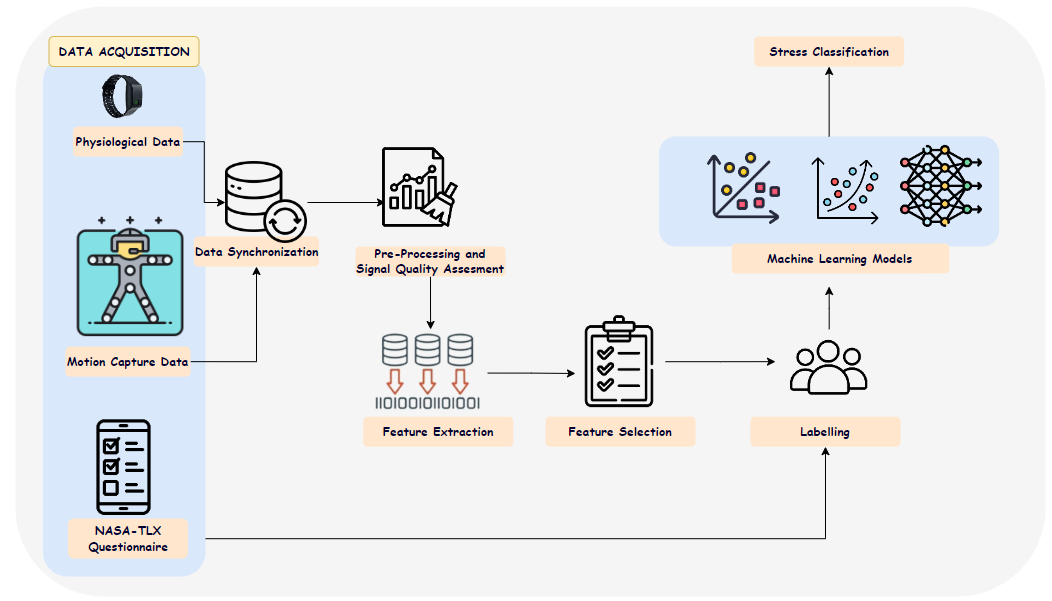
\includegraphics[width=\columnwidth]{images/Screenshot_5.png}
	\caption{Schematic of the experiment setup}
	\label{fig:netwrok}
\end{figure}

\section{Data Synchronization} \label{sec:Synchronization} \gls*{gptmo}
As previously eluded in section \ref{sec:expprot}, data synchronization is crucial to our experimental framework, ensuring the consistency
of data gathered from all the different sensors. In our setup, since the Empatica E4 wristband collects various physiological signals, including Blood Volume Pulse(BVP), Electrodermal Activity (EDA), Heart Rate (HR), and skin temperature at different frequencies as well as the motion capture system that tracks the participant's movements at a higher frequency. Given the varying sampling rates of these data sources, it's crucial to synchronize them to ensure they are comparable and accurate.

The Empatica E4 wristband samples at different rates for different signals: the Blood Volume Pulse (BVP) data is transmitted at 64Hz, while other metrics like EDA and temperature are transmitted at a lower rate of 4Hz. In contrast, the motion capture data, processed by the Motive software, is typically captured at a higher rate, around 120Hz. These discrepancies in sampling rates necessitate a careful synchronization approach.


Our synchronization strategy focuses on aligning diverse data streams to a unified frequency. Considering the need for detailed data and practical data processing constraints, we standardize all data streams to a frequency of 64Hz, matching the Blood Volume Pulse (BVP) rate from the Empatica E4. This standardization process involves downsampling the motion capture data, which originally records at a higher frequency of 120Hz. Simultaneously, for other signals like the Electrodermal Activity (EDA) and temperature, updating at a lower frequency of 4Hz, and acceleration data at 32Hz, we use a forward-filling approach, carrying their most recent values until an update occurs.

A specialized ROS node is responsible for this synchronization.  By using the BVP rate as the master reference, the node ensures that both physiological and motion data are synchronized in time. This alignment is key for an integrated and comprehensive analysis of the participant's responses, providing a dataset that accurately reflects both the physiological states and physical movements.

Once synchronized, the data is then published to a ROS topic, typically /aggregated\_data. This topic carries a comprehensive stream of information that combines detailed physiological measures with precise motion data. This rich dataset forms the foundation for subsequent phases of analysis in our study, such as feature extraction and stress detection.

\section{Pre-Processing} \gls*{gptmo}
Pre-processing is a crucial step in the analysis of data from physiological sensors and motion capture systems, as it prepares the raw data for subsequent processing and analysis phases. This section outlines the key aspects of pre-processing in our study.

\subsection*{Data Filtering} \label{sec:data_filtering}

In the pre-processing phase of our study, data filtering plays a crucial role in refining the quality of the signals gathered from the physiological sensors and motion capture systems. This step involves applying specific filtering techniques to the raw data to remove any unwanted data, thereby enhancing the signal's clarity and usability for further analysis.

The primary objective of data filtering is to isolate the significant aspects of the signal while eliminating any unwanted noise or interference. Depending on the nature of the signal and the type of noise present, different filtering methods are employed. For instance, we use N-th order Butterworth filters, which are effective in retaining the desired frequency range while attenuating frequencies outside this range. The Butterworth filter is known for its smooth frequency response and is particularly useful in physiological signal processing where preserving the integrity of the signal is crucial.

Each signal type dictates specific filter parameters like filter order, cutoff frequencies, and filter type (lowpass, highpass, or bandpass). This careful selection ensures the final signal is representative of the true physiological data crucial for accurate analysis.

\subsection*{Data Normalization}
Normalization is a critical step in data pre-processing aswell, particularly when dealing with signals of varying magnitudes or scales. Our approach involves applying a normalization process to each input signal, which standardizes the range of data values. This step is essential for comparing and combining data from different sensors effectively.

The method we use for normalization is primarily the 'z-score' method. This technique transforms the data to have a mean of zero and a standard deviation of one. By doing so, it ensures that each signal contributes equally to the analysis, irrespective of their original scale or distribution. This standardization is crucial for machine learning models, as it enhances algorithm performance and prevents any single feature from dominating due to its scale.

Normalization also aids in mitigating the impact of outliers, as it brings all data points onto a common scale, making them more suitable for analysis.

\begin{comment}
\subsection*{Peak Detection}
Peak detection is a method used to identify significant local maxima (peaks) and minima (troughs) in the data, which can represent important events or changes. In the context of stress detection, for instance, identifying peaks in heart rate or GSR signals can be indicative of moments of heightened stress or arousal. Efficient peak detection algorithms are crucial for accurately identifying these critical points in the data. Analyzing the frequency and intensity of these peaks can provide valuable insights into the physiological response patterns of the participants, such as the frequency of stress episodes or the degree of response to different stimuli.
\end{comment}

\subsection*{Signal Quality Assessment}
\label{sec:signal_quality_assessment}

Signal quality assessment is an integral part of the preprocessing phase to ensure the reliability and accuracy of data collected from sensors, which is fundamental for accurate analysis. Various methods are employed to assess the quality of signals, each targeting specific types of anomalies or artifacts.

\paragraph{Detection of Clipped Segments:}
This method involves identifying segments in the signal that are clipped or truncated. Clipping often occurs when the signal amplitude reaches the sensor's recording capacity limits. By setting thresholds for positive and negative clipping, the method detects and marks these segments, facilitating their exclusion or correction .

\paragraph{Detection of Flatline Segments:}
This method identifies flatline segments where the signal shows minimal variation over a period. Such segments can indicate sensor displacement or malfunction. The method identifies these periods by assessing the duration of flatness and the threshold for change in signal amplitude, helping exclude non-physiological data from the analysis.


Each method plays a crucial role in verifying the integrity of the signal data. Identifying and addressing issues like clipping, flatlining, and inconsistent patterns, signal quality assessment ensures that subsequent data analysis stages are based on accurate and reliable data.



\subsection*{Baseline Correction}
\label{sec:baseline_correction}

Baseline correction forms a pivotal part of our data normalization strategy, particularly tailored for participant-specific physiological data. This approach is centered around the concept of adjusting the data relative to each participant's baseline physiological state, typically captured during a rest period prior to the experimental tasks. This preparatory measure establishes a reference point against which subsequent physiological responses are compared.
In the baseline correction process, we begin by computing the average values of physiological signals recorded during the baseline phase before the start of the experiment. This baseline phase is critical as it represents a period of rest where the participant's physiological state is unaffected by experimental stressors. By establishing this baseline, we are able to set a reference point that reflects the participant's normal physiological state. Subsequently, we adjust the data points collected during the active phases of the experiment relative to these baseline averages. This adjustment is a normalization process that centers the data around a personalized zero point, effectively accounting for individual physiological variations. The core advantage of baseline correction lies in its ability to mitigate the influence of inter-individual variability on the physiological measurements. Since each participant's baseline state can vary significantly due to factors like inherent physiological differences, stress levels, and environmental conditions, normalizing data against this baseline ensures a more accurate and personalized assessment of stress responses.
This method ensures that the changes observed in the physiological data during the experiment are indicative of the participant's response to the experimental conditions, rather than being a reflection of their baseline physiological state.

\subsection*{Signal Segmentation}
\label{sec:signal_segmentation}
In our research, the segmentation of physiological and motion capture data into windows was a crucial part of the preprocessing. This process involved breaking down the continuous data streams into smaller, manageable windows for detailed analysis. The selection of window size and step size was critical, and was tailored based on the characteristics of the signal and the objectives of our analysis.

The window size was carefully chosen to capture relevant physiological and behavioral patterns within each segment, balancing the need to encapsulate meaningful data against the computational demands of processing. The step size determined the overlap between these windows, ensuring continuity and that no significant transient events were missed.

Accounting for the sampling rate of each signal was vital in customizing the segmentation process appropriately. This flexible approach was key to accommodating different types of signals, ensuring that the window size was appropriate for the length of the signal and that the segmentation parameters were compatible with each signal's nature.

Segmenting data into windows enabled us to convert the ongoing data streams into a format suitable for comprehensive analysis. This structured approach facilitated subsequent computational processes, including feature extraction and pattern recognition, essential for robust stress detection and analysis. This method of using windows in data segmentation is fundamental in ensuring that each part of the continuous data stream is analyzed effectively, allowing for a thorough understanding of stress indicators within the dataset.

\section{Feature Extraction} \gls*{gptmo}
Feature Extraction and Selection play a pivotal role in the effectiveness of machine learning models, especially in the context of human stress recognition. Feature extraction involves deriving meaningful attributes from the raw data collected. The type of features extracted can vary widely, including statistical features, time-domain, frequency-domain, as well as linear versus non-linear features.

The complexity of these features can range from basic statistical measures like mean, median, minimum, and maximum, to more intricate features based on specific data modalities. Each sensor used in stress detection may yield a unique set of features, contributing to the overall data analysis and model accuracy. The selection and application of these features are crucial, as they directly impact the classification stage, ultimately influencing the model's performance in stress recognition.

\subsection{EDA-Electrodermal Activity}

Electrodermal Activity (EDA), also known as galvanic skin response (GSR), is a sensitive measure of emotional and physiological arousal. It primarily consists of two components: tonic (Skin Conductance Level, SCL) and phasic (Skin Conductance Response, SCR).As explained in Section \ref*{subsec:EDAtheory} the tonic component represents baseline levels of skin conductance, reflecting slow changes in arousal state. The phasic component, on the other hand, captures rapid fluctuations in response to specific stimuli or events.


After the usual process of filtering and normalizing the signal aswell checking the quality of the signal we first decompose the EDA signal into its tonic and phasic components using continuous decomposition analysis. This process allows us to separately analyze the steady-state (SCL) and transient (SCR) aspects of skin conductance.
The decomposition is typically carried out using highpass filtering techniques, ensuring that each component accurately represents the underlying physiological processes.
\begin{figure}[hb]
	\centering
	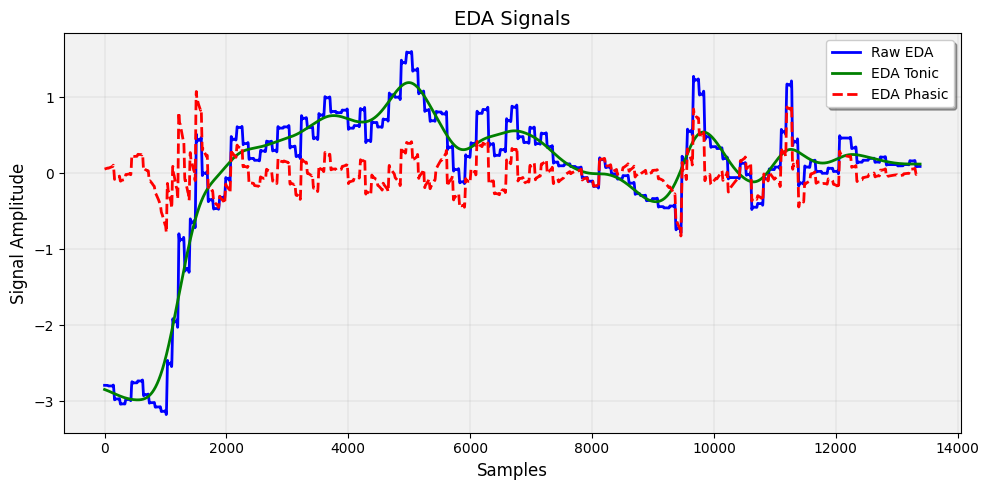
\includegraphics[width=\columnwidth]{images/eda.png}
	\caption{EDA}
	\label{fig:eda sig}
\end{figure}

We conducted a comprehensive review and comparison of various EDA features, ultimately selecting those most relevant to our research objectives. This meticulous selection process, influenced by a thorough examination of nearly 40 distinct EDA features as outlined by previous studies \textcite{EDAFeatures}, enabled us to tailor our feature set.

From the decomposed EDA data, a variety of time domain statistical features can be extracted. These include mean ($\mu$), standard deviation ($\sigma$), coefficient of variance (CV), variance ($\sigma^2$), and kurtosis ($\beta$) from the phasic component.

Mean ($\mu$) provides a measure of the central tendency of the SCR amplitudes.
Standard deviation ($\sigma$) and variance ($\sigma^2$) capture the variability or dispersion around the mean.
The coefficient of variance (CV) offers a normalized measure of dispersion relative to the mean.
Kurtosis ($\beta$) evaluates the peakedness or flatness of the distribution of SCR amplitudes.

In addition to time-domain features, we analyze the EDA signal in the frequency domain. Furthermore, frequency-domain features like spectral power in specific bands (f1sc, f2sc, f3sc) and the overall energy and entropy of the signal gave us a spectrum-based view of the EDA responses. By analyzing these features, we could discern patterns and rhythms in the EDA that are not immediately apparent in the time-domain.


Detecting and analyzing peaks in the phasic component (SCRs) is crucial. Peak amplitude, frequency, and their inter-relationships can be strong indicators of emotional and cognitive stress responses.

By examining both tonic and phasic components, we can understand the sustained arousal level (SCL) and the specific responses to stimuli (SCR). The correlation between these components can provide valuable insights into how sustained stress levels influence responses to immediate stimuli.
From the tonic component, which encapsulates the underlying level of arousal, we calculated the mean, capturing the central tendency over time, and the standard deviation, offering insights into the variability around this mean. The maximum and minimum values, along with the range, provided us with the extremes of the EDA signal, painting a picture of the breadth of responses.

From the phasic component, we focused on the Skin Conductance Responses (SCRs) to discern more rapid changes associated with specific stimuli. We extracted features like SCR amplitude, which reflects the intensity of the response, and the frequency of these SCRs, indicating how often these responses occur. The kurtosis of SCR amplitudes, a measure of the 'tailedness' of the distribution, gave us an understanding of how peaked or flat the distribution of responses was, while the skewness indicated any asymmetry, offering clues about the predominant direction of the response distribution.

We also looked at the root mean square (SCR RMS), which is a measure of the signal's magnitude, and the arc length (SCR Arc Length), providing a summative measure of the signal's complexity over a given period. The integral of the SCR signal (SCR Integral) was calculated to understand the total magnitude of these phasic responses over time. These features, alongside others like SCR momentum, which is akin to the second moment of the distribution, provided a comprehensive statistical breakdown of the phasic EDA signals.

\textcite[]{EDAFeatures}  we reviewed and compared amlost 40 different EDA features, the features extracted selected with the help of this.

\subsection{Body Features}
Since we captured human motion using the motion capture system, we selected 13 key points from the 25 marker points used by the system, focusing on the upper body. The chosen points were Hip, Ab, Chest, Neck, Head, Left Shoulder (LShoulder), Left Upper Arm (LUArm), Left Forearm (LFArm), Left Hand (LHand), Right Shoulder (RShoulder), Right Upper Arm (RUArm), Right Forearm (RFArm), and Right Hand (RHand). These points were strategically selected to comprehensively capture upper body movements. The arrangement of these points is depicted in Fig \ref{fig:human}

\begin{figure}[h]
	\centering
	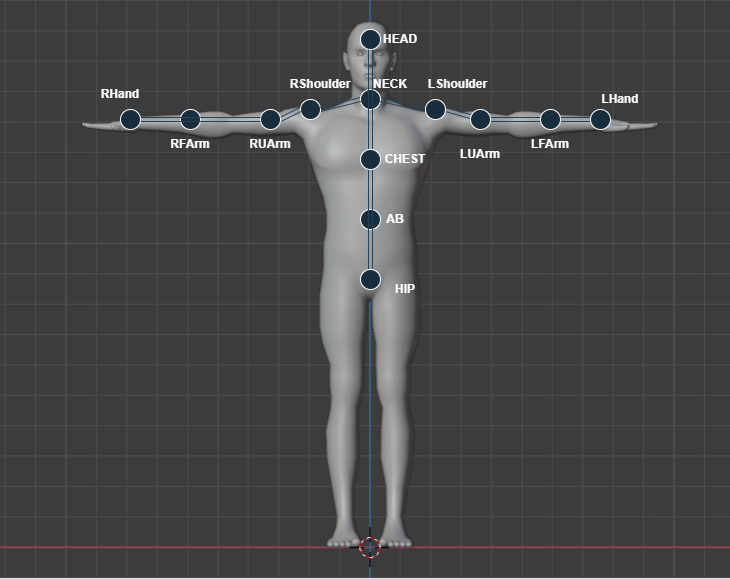
\includegraphics[width=0.8\columnwidth]{images/human.png}
	\caption{13 points from the motion capture} 
	\label{fig:human}
\end{figure}


%\textcite[postnote]{HARRIGAN19851161} HARRIGAN19851161
\subsection*{Self Touching} 
Previous studies, such as the one referenced in \textcite{10.1371/journal.pone.0043571}, indicate that body posture and body language can be valuable indicators of stress. In line with this, we also explored body language cues such as self-touching, which \textcite{HARRIGAN19851161}suggests can be indicative of negative affect, such as anxiety or discomfort. Specifically, we focused on face and head touching as potential stress indicators.

To determine if a person is touching her face, we compute the hand-head and the hand-neck distances. If one of these distances is below a given threshold, we consider that the person is face touching. The number of occurrences (FTC) and the average duration (FTMD) of these face touching events are used as features. 

To determine gestures such as face touching, \texttt{/tf} data, which typically includes the position and orientation of each joint in space, can be utilized to calculate the distance between any two points. For example, if you have the coordinates of the right hand (\texttt{RHand}) and the head (\texttt{HEAD}), you can compute the Euclidean distance between these two points at each time frame to detect when the hand is close enough to the head to indicate potential face touching.

Let's define the 3D coordinates for the right hand and head at time $t$ as:
\begin{itemize}
\item $P_{\text{RHand}}(t)$ for the position of the right hand at time $t$, with coordinates $(x_{\text{RHand}}(t), y_{\text{RHand}}(t), z_{\text{RHand}}(t))$,
\item $P_{\text{HEAD}}(t)$ for the position of the head at time $t$, with coordinates $(x_{\text{HEAD}}(t), y_{\text{HEAD}}(t), z_{\text{HEAD}}(t))$.
\end{itemize}

The distance between the right hand and the head at time $t$ is then calculated with the formula:

\begin{equation}
D_{\text{RHand-HEAD}}(t) = \sqrt{(x_{\text{RHand}}(t) - x_{\text{HEAD}}(t))^2 + (y_{\text{RHand}}(t) - y_{\text{HEAD}}(t))^2 + (z_{\text{RHand}}(t) - z_{\text{HEAD}}(t))^2}
\end{equation}

If this distance, $D_{\text{RHand-HEAD}}(t)$, is less than a certain threshold, denoted as $\theta$, it suggests that the right hand is in proximity to the head, indicating potential face touching.

To determine the occurrence of face touching, you would track when this distance becomes less than the threshold $\theta$ and also ensure that the hand remains within this threshold for a certain duration to count as an occurrence. The distance for the left hand can be calculated in a similar manner.

To compute the number of occurrences (\texttt{FTC-Face Touching Count}) and the average duration (\texttt{FTMD-Face Touching Mean Duration}) of face touching is shown in Algorithm \ref{alg:face_touching}.

    \begin{algorithm}
        \caption{Face Touching Detection}
          \label{alg:face_touching}
        \begin{algorithmic}[1]
          \Require{Set of time-stamped positions from the \texttt{/tf} topic, Threshold distance $\theta$}
          \Statex
          \Function{DetectFaceTouching}{}
            \State Initialize $FTC \gets 0$ \Comment{Occurrences of face touching}
            \State Initialize $TotalDuration \gets 0$ \Comment{Total duration of face touching events}
            \State Initialize $FTMD \gets 0$ \Comment{Mean duration of face touching events}
            
            \For{each time stamp $t_i$ in \texttt{/tf} topic}
              \State Calculate $D_{RHand-Head}(t_i)$ and $D_{LHand-Head}(t_i)$
              
              \If{$D_{RHand-Head}(t_i) < \theta$ \textbf{or} $D_{LHand-Head}(t_i) < \theta$}
                \State Start duration counter
                \State $FTC \gets FTC + 1$
              \EndIf
              
              \If{either distance exceeds $\theta$}
                \State Stop duration counter
                \State Add duration to $TotalDuration$
              \EndIf
            \EndFor
            
            \If{$FTC > 0$}
                \State $FTMD \gets \frac{TotalDuration}{FTC}$ \Comment{Calculate mean duration}
            \EndIf
            \State \textbf{return} $FTC$, $FTMD$
          \EndFunction
        \end{algorithmic}
      \end{algorithm}

      
\subsection*{Sudden Movement }
\label{subsec:sudden_movement_analysis}

\textcite{hyperactivity} suggested another way in which motion data can be used to assess stress.
Sudden movements, or abrupt changes in body motion, can be indicative of stress responses. These movements are characterized by significant deviations from a person's regular movement patterns and can be quantitatively assessed using motion capture data. The following equations describe the computational process used to analyze sudden movements and infer stress.

\begin{equation}
m_j^k = \sum_{i=0}^{\tau-1} d_j^{k-i,k-i-1}
\label{eq:movement_joints}
\end{equation}

Equation~\ref{eq:movement_joints} defines the movement of the \( j^{th} \) joint within a time window \( \tau \) as the sum of the displacements between consecutive frames. 

\begin{equation}
\Delta_j^k = m_j^k - \mu_j
\label{eq:deviation_baseline}
\end{equation}

In Equation~\ref{eq:deviation_baseline}, \( \Delta_j^k \) represents the deviation of the \( j^{th} \) joint's movement from its baseline mean motion \( \mu_j \), calculated during a calibration phase.

\begin{equation}
a_j^k = 
\begin{cases} 
  \frac{\Delta_j^k}{\sigma_j} - 1 & \text{if } \Delta_j^k > \sigma_j \\
  0 & \text{otherwise}
\end{cases}
\label{eq:activity_evaluation}
\end{equation}

Equation~\ref{eq:activity_evaluation} assesses the activity level \( a_j^k \) for the \( j^{th} \) joint, taking into account the standard deviation \( \sigma_j \) as a threshold for sudden movement.

\begin{equation}
a_k = \min \left( 1, \frac{1}{N} \sum_{j=1}^{N} a_j^k \right)
\label{eq:descriptor_sudden_movement}
\end{equation}

Finally, Equation~\ref{eq:descriptor_sudden_movement} calculates the overall level of sudden movement at time instance \( k \) by averaging the activities across all joints, thus providing a descriptor of hyperactivity or sudden movement.

This method allows for a comprehensive analysis of the motion data to identify periods of high activity that may correlate with stress responses.


While our study focused on the analysis of upper body movements for stress detection, it is important to note that other bodily cues can also be significant indicators of stress or anxiety. One such example is the rapid tapping or bouncing of one's feet, which is often a subconscious response to nervous energy or unease. Such movements are typically a form of self-soothing behavior that occurs when an individual is experiencing discomfort or stress.

Unfortunately, due to the scope of our motion capture system setup, we restricted our tracking to the upper body and therefore could not capture lower body movements, such as foot tapping or leg bouncing. These actions could potentially provide additional insights into a participant's stress levels and offer a more comprehensive understanding of physical stress responses.

Including lower body data in future studies could enhance the detection and analysis of stress indicators, allowing for a fuller picture of the physiological and behavioral state of an individual under stress. This would enable us to capture a wider range of stress-related behaviors and potentially increase the accuracy and reliability of stress detection in real-time scenarios.
\section{Classification /Stress Detection/}

% !TeX spellcheck = en_US
% !TeX encoding = UTF-8
\chapter{Result}

%\section{Latex distributions and editors}
% !TeX spellcheck = en_US
% !TeX encoding = UTF-8
\chapter{Conclusion}
\section{Discussion}

Discussion of the results compared to the objective--- Limitation(sujective ground thruth)---- Future work(improvement in detection model, real time system schematic and breif, parameter tuning of the controller etc etc)
and then conclusion


\section{Analysis of ground truth}

\begin{figure}[!htbp]
	\centering
	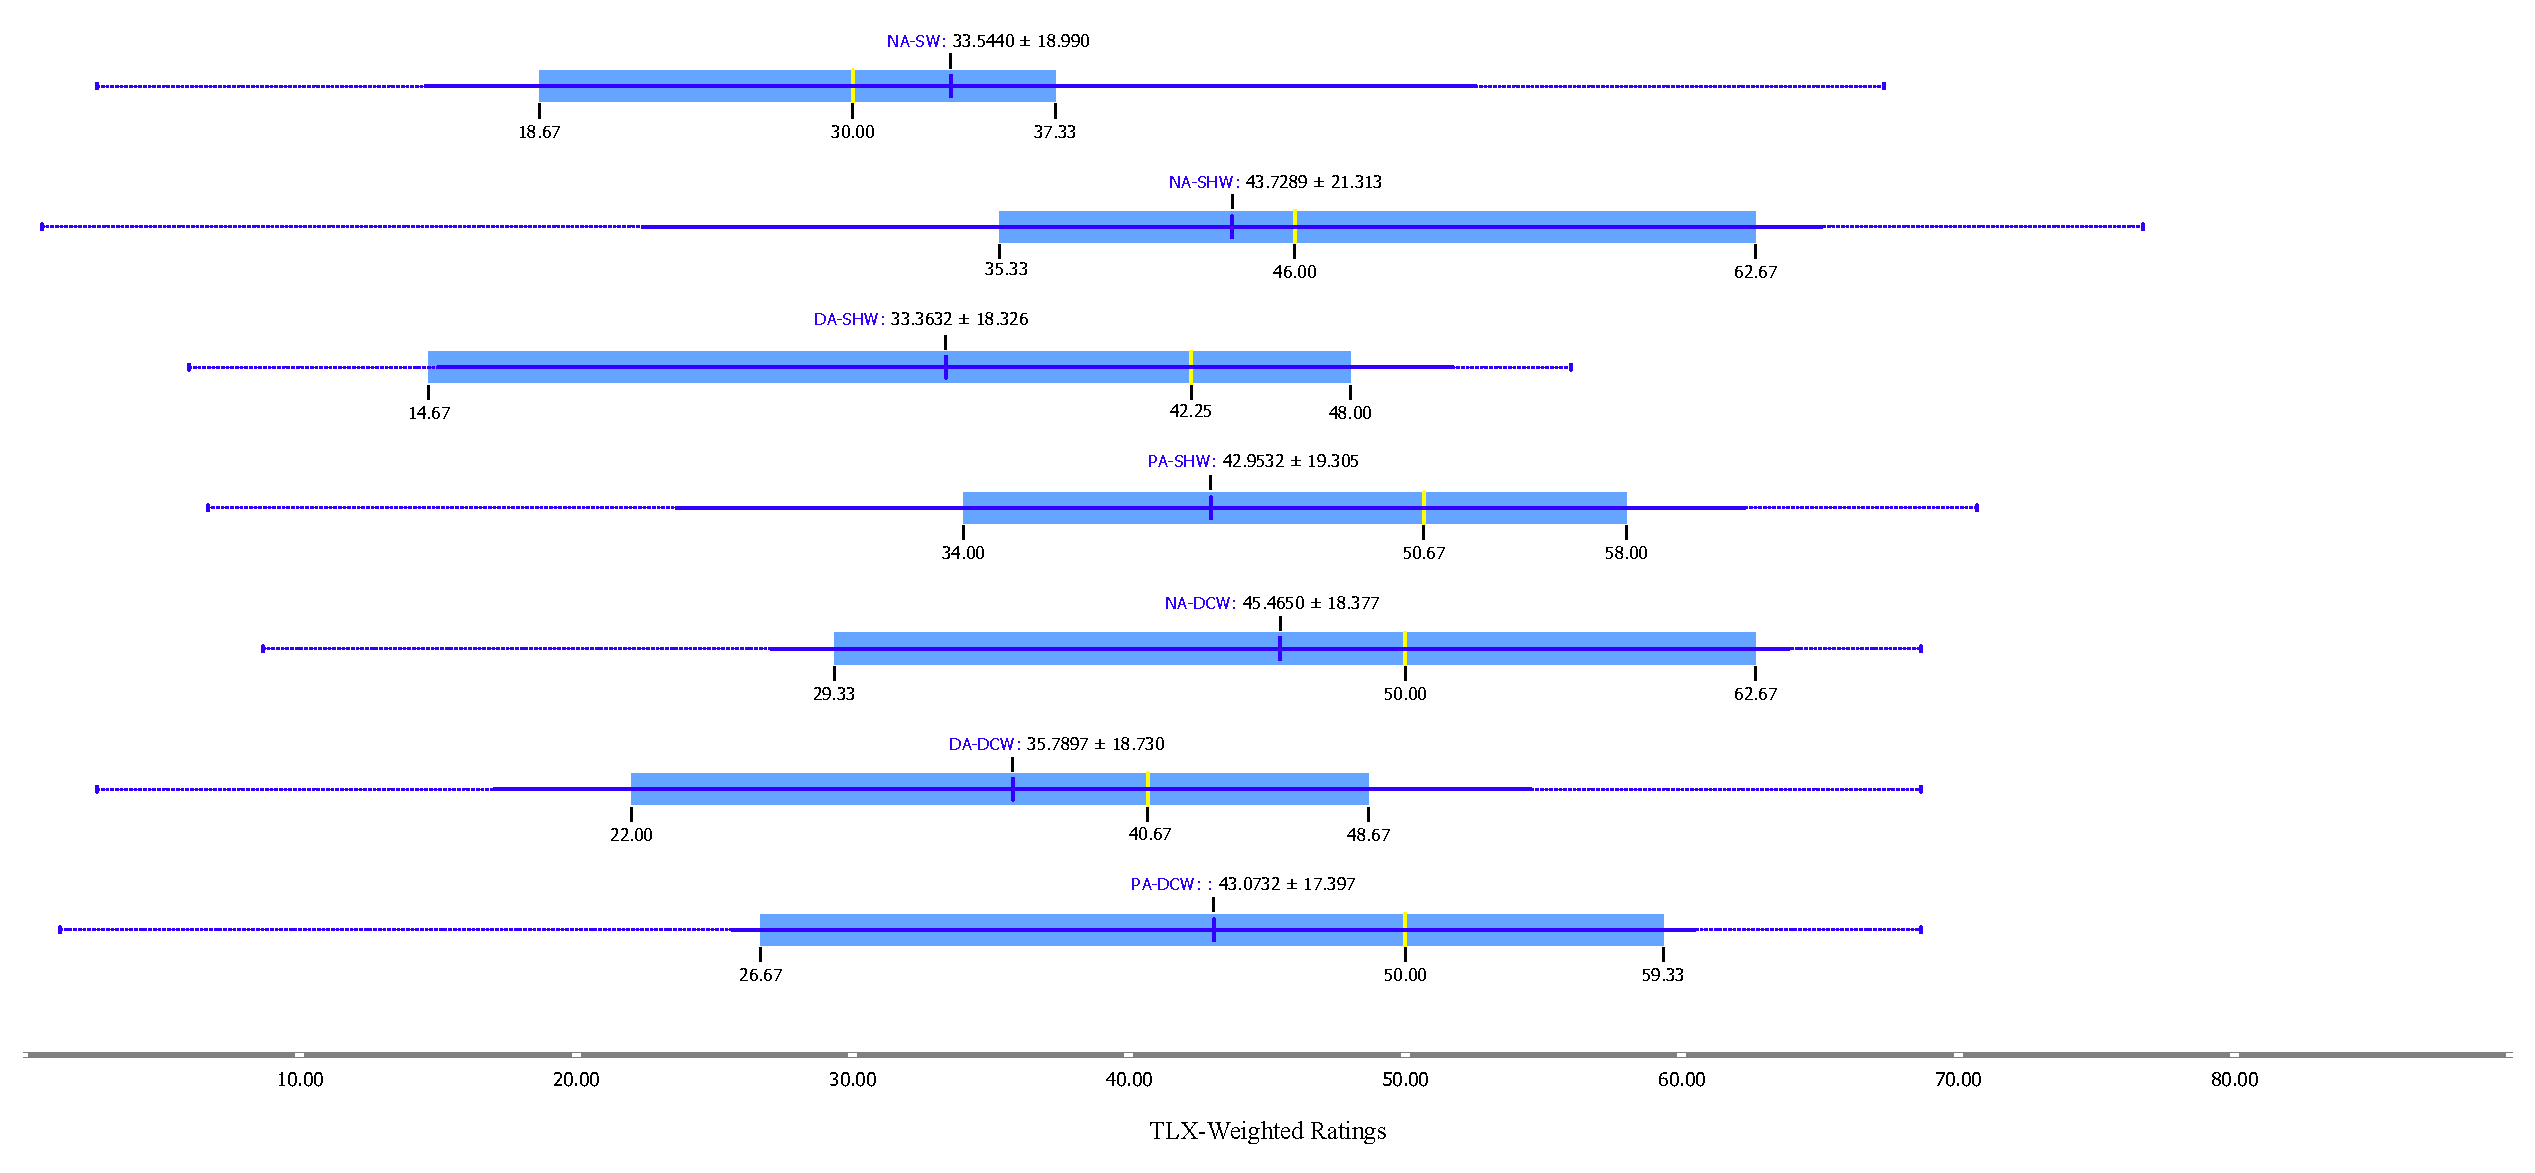
\includegraphics[width=\columnwidth]{images/tlx.pdf}
	\caption{}
	\label{fig:netwrok}
\end{figure}

In our research on stress analysis, we primarily relied on subjective measures for labeling and establishing ground truth. While many previous studies have successfully employed this approach, it is important to acknowledge that subjective ratings can be influenced by a variety of factors. These influences could range from individual perception differences to contextual and environmental factors impacting a participant's response. Consequently, reducing the complex and multifaceted nature of stress into a three-class system based on subjective assessments might lead to oversimplifications of the nuanced nature of stress.


To bolster the reliability of our labeling process, we undertook an initiative to crossvalidate our labels with other physiological or behavioral stress indicators. This crossvalidation aimed to correlate our subjective stress labels with objective measures, such as mean skin conductance response meanscr and heart rate meanhr. It is crucial to note that this assumption that meanscr and meanhr directly indicate stress was specifically for the purpose of this crossvalidation exercise and not a general assumption throughout our project.


Given that physiological features like meanscr and meanhr are integral inputs of our stress detection model, they could not be directly used for labeling the stress categories. This constraint necessitated our reliance on subjective measures for labeling. However, by attempting to correlate these objective physiological indicators with our subjective labels, we sought to add a layer of validation to our approach.


Before delving into our results, it is imperative to discuss some critical caveats about our methodology. Our reliance on subjective ratings, though methodologically sound in many aspects, does not entirely capture the reliable ground truth of stress. The subjective nature of these ratings means they are susceptible to various influencing factors, which might not always align perfectly with physiological manifestations of stress. This acknowledgment is crucial for a comprehensive understanding of our findings and their interpretation.


Our approach, while aligned with standard practices in stress research, does acknowledge the limitations inherent in using subjective measures for stress categorization. By attempting cross-validation with physiological data, we endeavored to enhance the robustness of our methodology. Nevertheless, the complexities and intricacies of stress as a psychological and physiological phenomenon demand careful consideration and interpretation of our results.


\section{Future work}

%\section{Latex distributions and editors}

% ##########################################################################
% BIBLIOGRAPHY
% ##########################################################################

% Normal bibliography containing all cited references
\printbibliography[notcategory=pub,notcategory=pubco,notcategory=pubother,notcategory=pubotherco,notcategory=thes,notcategory=media,notcategory=pat,notcategory=pgs]

% Extra bibliography in case of a PhD containing all supervised theses, published work and media
\iftoggle{thesis_phd}{%
	\clearpage
	% !TeX encoding = UTF-8

% sort by year (decending)
\newrefcontext[sorting=ydnt]

%% Own publications
\addpub{own.mustermann2014}
\addpub{own.mustermann2017}

\printbibliography[env=pubenv,heading=pub,category=pub]%
\clearpage

%% Co-authored publications
\addpubco{own.bertram2015}
\addpubco{own.bertram2018}

\printbibliography[env=pubenv,heading=pubco,category=pubco]%
\clearpage

%% Additional publications
\addpubother{own.mustermann2016}

\printbibliography[env=pubenv,heading=pubother,category=pubother]%
\clearpage

%% Co-authored Additional publications
\addpubotherco{own.bertram2016}

\printbibliography[env=pubenv,heading=pubotherco,category=pubotherco]%	
\clearpage

%% Supervised theses
\addthesis{mt.musterfrau2015}
\addthesis{bt.wayne2017}
	
\printbibliography[env=pubenv,heading=thes,category=thes]%
\clearpage

%% Project groups
\addpg{pg2017}

\printbibliography[env=pubenv,heading=pgs,category=pgs]%
\clearpage

%% Patents
\addpat{Wayne2022}

\printbibliography[env=pubenv,heading=pat,category=pat]%}

% ##########################################################################
% APPENDIX
% ##########################################################################

% !TeX encoding = UTF-8
\chapter{\iftoggle{lang_eng}{Appendix}{Anhang}}
\label{app:Anhang1}


\begin{table}[H]
    \centering
    \resizebox{\textwidth}{!}{%
    \begin{tabular}{|l|l|l|}
    \hline
    \textbf{Feature Category} & \textbf{Feature} & \textbf{Description} \\ \hline
    \multirow{8}{*}{Statistical Features} & eda\_mean & Mean of EDA signal \\ 
     & eda\_std & Standard deviation of EDA signal \\ 
     & eda\_max & Maximum value of EDA signal \\
     & eda\_min & Minimum value of EDA signal \\
     & eda\_range & Range of EDA signal (max - min) \\
     & eda\_kurtosis & Kurtosis of EDA signal \\
     & eda\_skew & Skewness of EDA signal \\
     & eda\_momentum & Overall momentum of EDA signal \\ \hline
    \multirow{5}{*}{Frequency-Domain Features} & eda\_f1sc, eda\_f2sc, eda\_f3sc & Frequency-specific components \\
     & eda\_Energy & Total energy of EDA signal \\
     & eda\_Entropy & Entropy of EDA signal \\
     & eda\_max\_freq & Maximum frequency in EDA signal \\ \hline
    \multirow{15}{*}{SCR Features} & scr\_mean & Mean of SCR signal \\
     & scr\_std & Standard deviation of SCR signal \\
     & scr\_max, scr\_min, scr\_range & Various measures of SCR \\
     & scr\_kurtosis, scr\_skew & Kurtosis and Skewness of SCR \\
     & scr\_momentum & Overall momentum of SCR signal \\
     & scr\_activity, scr\_complexity & Activity and complexity measures \\
     & scr\_mobility, scr\_rms & Mobility and RMS of SCR \\
     & scr\_acr\_length, scr\_integral & ACR length and integral of SCR \\
     & scr\_average\_power & Average power of SCR \\
     & scr\_f1sc, scr\_f2sc, scr\_f3sc & Frequency-specific components of SCR \\
     & scr\_Energy & Total energy of SCR signal \\
     & scr\_Entropy & Entropy of SCR signal \\
     & scr\_max\_freq & Maximum frequency in SCR signal \\ \hline
    \multirow{8}{*}{SCL Features} & scl\_mean, scl\_std & Mean and Standard deviation of SCL \\
     & scl\_max, scl\_min & Maximum and Minimum value of SCL \\
     & scl\_range & Range of SCL \\
     & scl\_kurtosis, scl\_skew & Kurtosis and Skewness of SCL \\
     & scl\_momentum & Overall momentum of SCL \\ \hline
    \end{tabular}
    }
    \caption{EDA Features Overview}
    \label{tab:eda_features}
    \end{table}
    
    \begin{table}[H]
        \centering
        \resizebox{\textwidth}{!}{%
        \begin{tabular}{|l|l|l|}
        \hline
        \textbf{Parameter Type} & \textbf{Feature} & \textbf{Description} \\ \hline
        \multirow{19}{*}{Time-domain HRV} & mean\_nni & Mean of peak to peak intervals \\ 
         & sdnn & Standard deviation of peak to peak intervals \\ 
         & rmssd & Root mean square of successive differences \\
         & sdsd & Standard deviation of successive differences \\
         & nni\_50 & Number of pairs of intervals differing by more than 50 ms \\
         & pnni\_50 & Ratio of nni\_50 to total number of intervals \\
         & nni\_20 & Number of pairs of intervals differing by more than 20 ms \\
         & pnni\_20 & Ratio of nni\_20 to total number of intervals \\
         & cvnni & Ratio of sdnn to mean\_nni \\
         & cvsd & Ratio of rmssd to mean\_nni \\
         & median\_nni & Median of successive differences \\
         & range\_nni & Range of peak to peak intervals \\
         & mean\_hr & Mean heart rate \\
         & min\_hr & Minimum heart rate \\
         & max\_hr & Maximum heart rate \\
         & std\_hr & Standard deviation of heart rate \\
         & mad\_nni & Mean absolute deviation of intervals \\
         & mcv\_nni & Ratio of mead\_nni to median\_nni \\
         & iqr\_nni & Interquartile range of intervals \\ \hline
        \multirow{12}{*}{Frequency-domain HRV} & vlf & Very low frequency power \\
         & lf & Low frequency power \\
         & hf & High frequency power \\
         & lf\_hf\_ratio & Ratio of lf to hf \\
         & total\_power & Sum of vlf, lf, and hf \\
         & lfnu & Normalized lf power \\
         & hfnu & Normalized hf power \\
         & lnLF & Log transformed low-frequency power \\
         & lnHF & Log transformed high-frequency power \\
         & vlf\_peak & Max peak in very low frequency band \\
         & lf\_peak & Max peak in low frequency band \\
         & hf\_peak & Max peak in high frequency band \\ \hline
        \multirow{9}{*}{Nonlinear HRV} & SD1 & SD of Poincare plot perpendicular to identity line \\
         & SD2 & SD of Poincare plot along the identity line \\
         & SD2\_SD1 & Ratio of SD2 to SD1 \\
         & CSI & Cardiac stress index \\
         & CVI & Cardiac vagal index \\
         & CSI\_modified & Modified cardiac stress index \\
         & ApEn & Approximate entropy of intervals \\
         & SampEn & Sample entropy of intervals \\ \hline
        \end{tabular}
        }
        \caption{PPG-HRV Features Overview}
        \label{tab:ppg_hrv_features}
        \end{table}
        



\begin{figure}[!htbp]
	\centering
	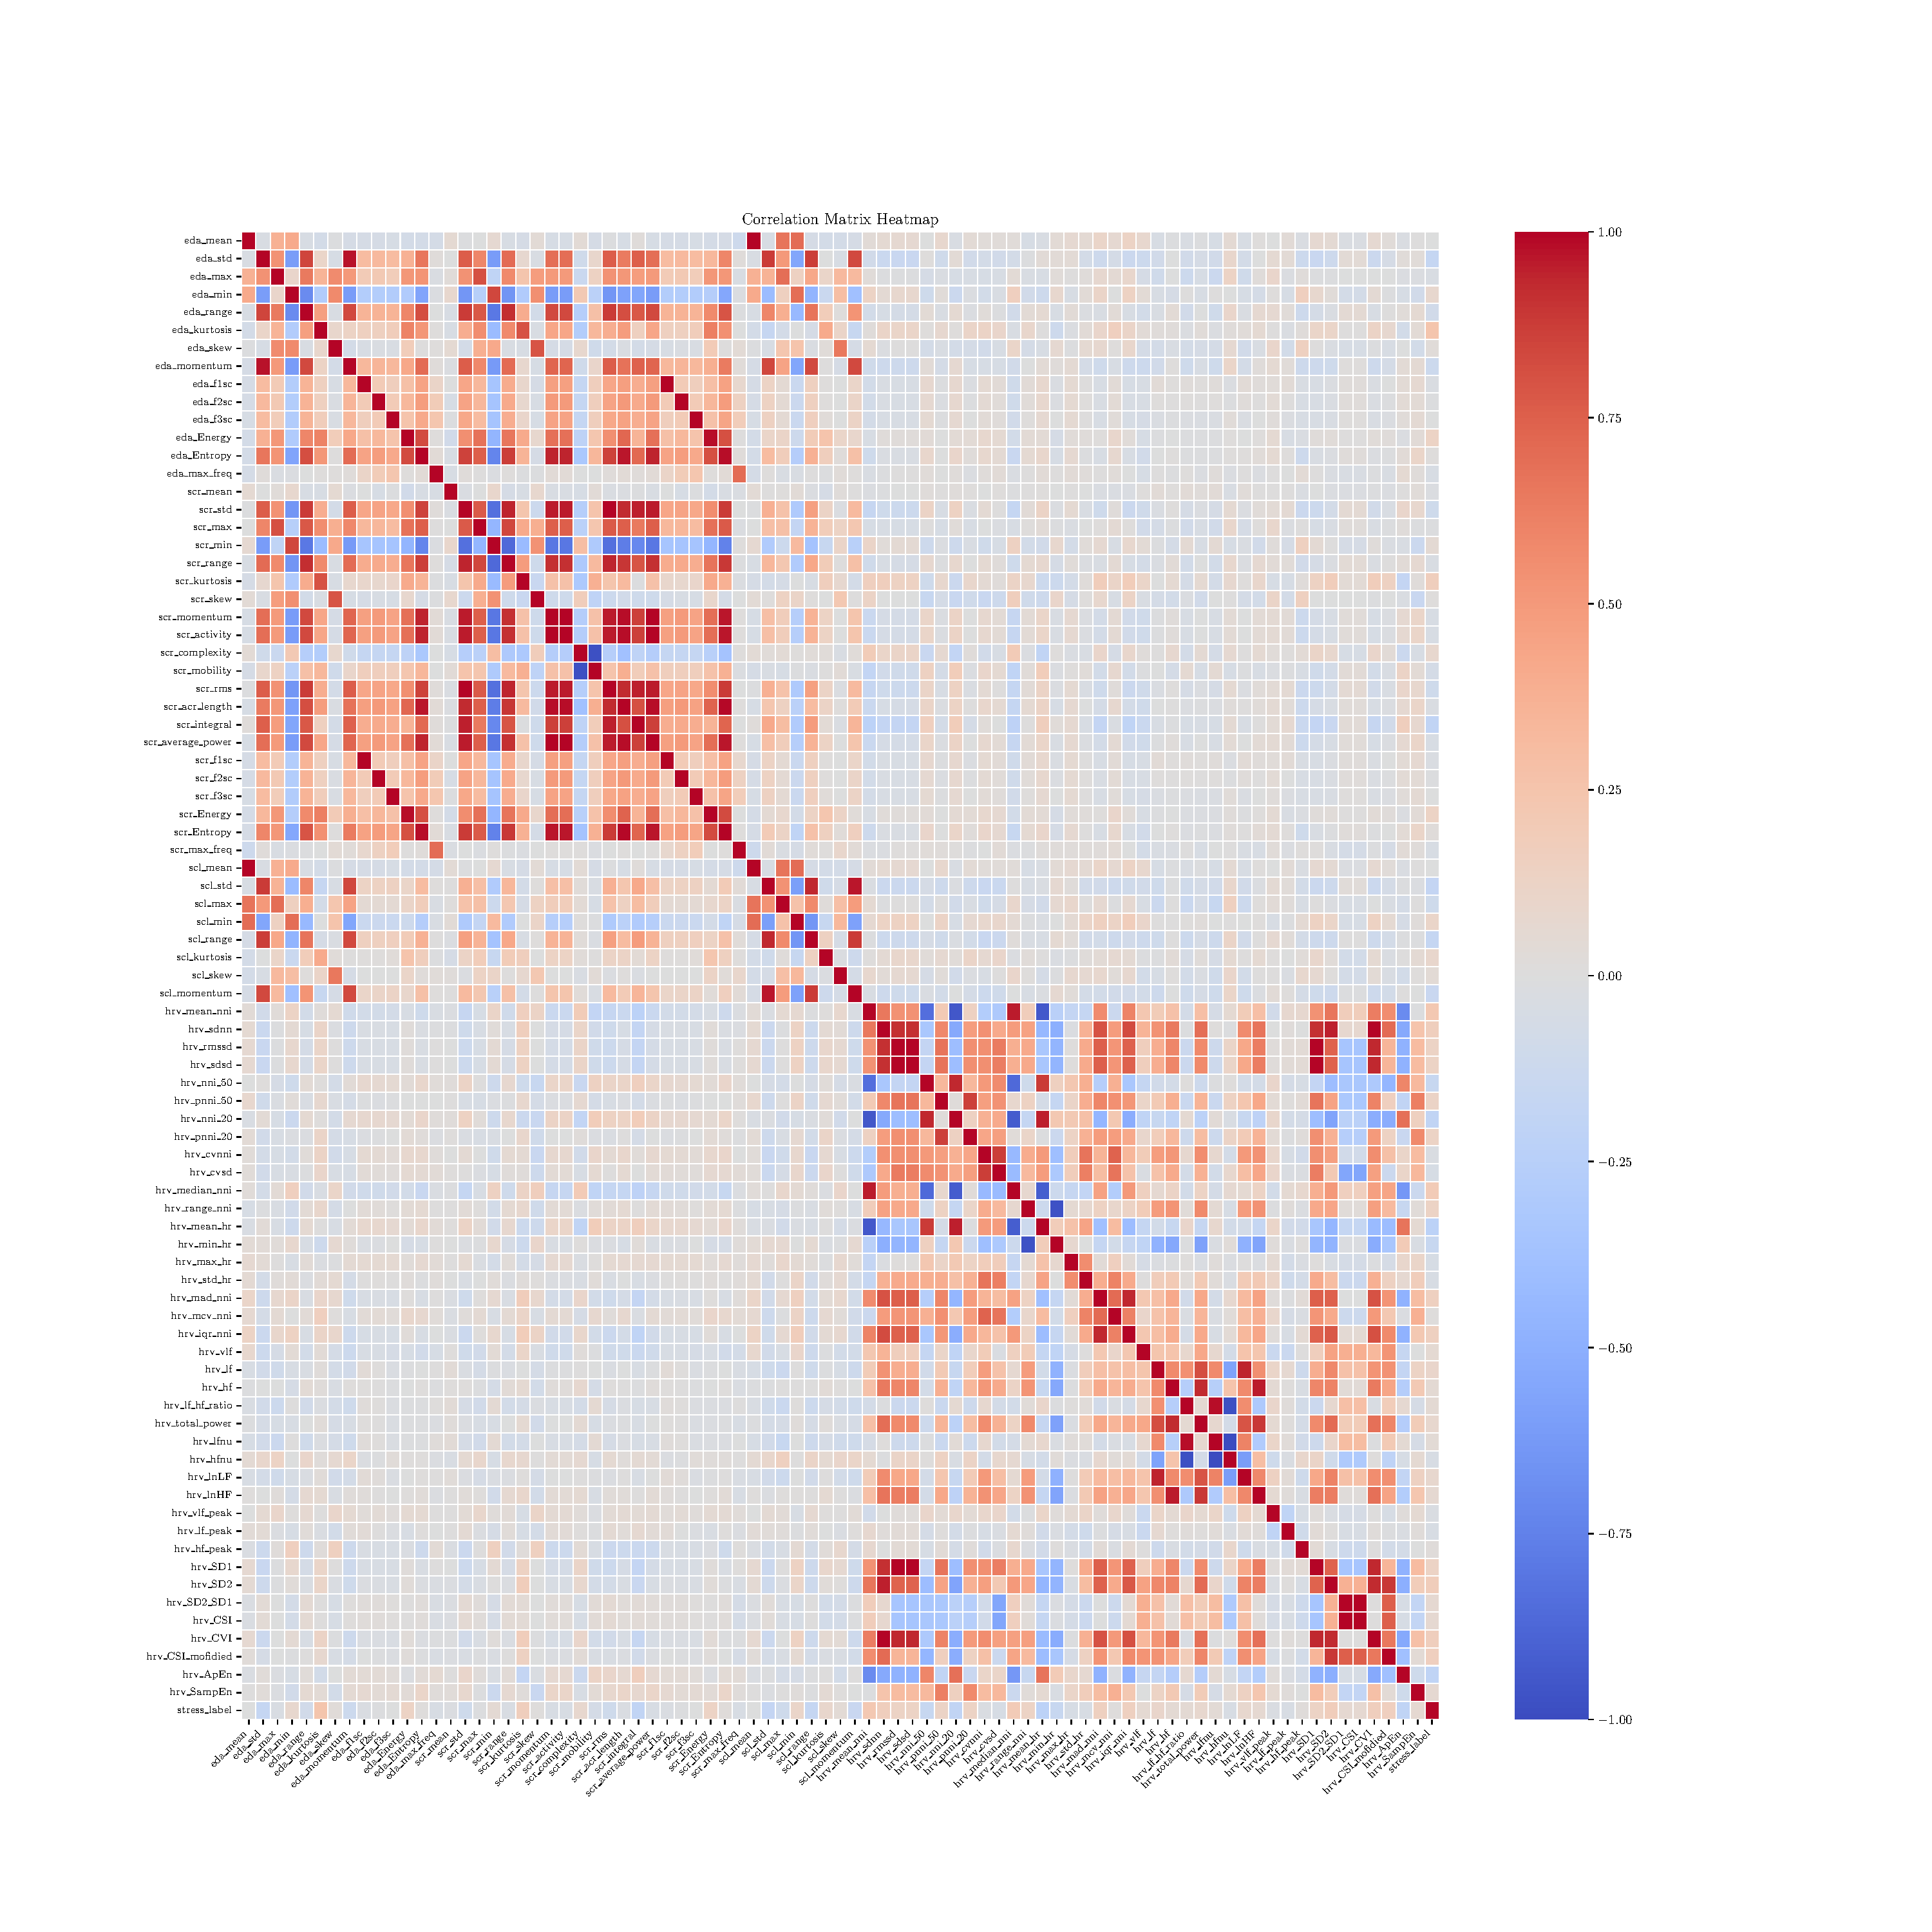
\includegraphics[width=\columnwidth]{images/correlation_matrix_heatmap.pdf}
	\caption{Correlation matrix for feature selection}
	\label{fig:netwrok}
\end{figure}



\newpage
\section{\iftoggle{lang_eng}{Usage of generative AI - Affidavit}{Erklärung zur Nutzung generativer KI-Modelle}}
\label{app:erklaerung}
\iftoggle{thesis_phd}{
    \begin{itemize}
        \item[$\square$] {\iftoggle{lang_eng}{not at all}{gar nicht}}
        \item[$\boxtimes$] {\iftoggle{lang_eng}{for correcting, optimizing, or restructuring the entire work (This eliminates the need for explicit marking of individual passages or sections, as this type of usage refers to the entire written work. Explicit marking in the text is not necessary, as this serves as the global indication.)}{zur Korrektur, Optimierung oder Umstrukturierung der gesamten Arbeit (Dies erübrigt eine explizite Markierung einzelner Passagen oder Abschnitte, da sich diese Art der Nutzung auf die gesamte schriftliche Ausarbeitung bezieht. Eine explizite Markierung im Text ist nicht notwendig, da hiermit die globale Kenntlichmachung erfolgt.)}}

        %Code
        \item[\ifglsused{gptco}{$\boxtimes$}{$\square$}] {\iftoggle{lang_eng}{Code optimization: Optimization or restructuring of software function}{Codeoptimierend: Optimierung oder Umstrukturierung von Software-Funktionen}}
        \item[\ifglsused{gptcg}{$\boxtimes$}{$\square$}] {\iftoggle{lang_eng}{Code generation: Creating entire software functions from a detailed functional description.}{Codegenerierend: Erstellung ganzer Software-Funktionen aus einer
        detailierten Funktionsbeschreibung}}
        \item[\ifglsused{gptcs}{$\boxtimes$}{$\square$}] {\iftoggle{lang_eng}{Substance generation in code: Generating entire software source code}{Code-Substanzgenerierend: Erzeugung ganzer Software-Quelltexte}}
        %Media
        \item[\ifglsused{gptmo}{$\boxtimes$}{$\square$}] {\iftoggle{lang_eng}{Media optimization: Correction, optimization, or restructuring of entire passages}{Medienoptimierend: Korrektur, Optimierung oder Umstrukturierung
        ganzer Passagen}}
        \item[\ifglsused{gptmg}{$\boxtimes$}{$\square$}] {\iftoggle{lang_eng}{Media generation: Creating entire passages from given content.}{Mediengenerierend: Erstellen ganzer Passagen aus vorgegebenem Inhalt}}
        \item[\ifglsused{gptms}{$\boxtimes$}{$\square$}] {\iftoggle{lang_eng}{Substance generation in media: Generating entire sections}{Medien-Substanzgenerierend: Erzeugung ganzer Abschnitte}}
        \item[\ifglsused{gptx}{$\boxtimes$}{$\square$}] {\iftoggle{lang_eng}{More, namely:}{Weiteres, nämlich:}}

    \end{itemize}
    \hrulefill

    \hrulefill

    \hrulefill

    \hrulefill

    {\iftoggle{lang_eng}{I assure that I have provided all usages completely. Missing or incorrect information may be considered an attempt to deceive.}{Ich versichere, alle Nutzungen vollständig angegeben zu haben. Fehlende oder fehlerhafte Angaben können als Täuschungsversuch gewertet werden.}}
    \\[10pt]
}
{
    \begin{itemize}
        \item[$\square$] {\iftoggle{lang_eng}{not at all}{gar nicht}}
        \item[$\boxtimes$] {\iftoggle{lang_eng}{for correcting, optimizing, or restructuring the entire work (This eliminates the need for explicit marking of individual passages or sections, as this type of usage refers to the entire written work. Explicit marking in the text is not necessary, as this serves as the global indication.)}{zur Korrektur, Optimierung oder Umstrukturierung der gesamten Arbeit (Dies erübrigt eine explizite Markierung einzelner Passagen oder Abschnitte, da sich diese Art der Nutzung auf die gesamte schriftliche Ausarbeitung bezieht. Eine explizite Markierung im Text ist nicht notwendig, da hiermit die globale Kenntlichmachung erfolgt.)}}

        %Code
        \item[$\boxtimes$] {\iftoggle{lang_eng}{Code optimization: Optimization or restructuring of software function}{Codeoptimierend: Optimierung oder Umstrukturierung von Software-Funktionen}}
        \item[$\boxtimes$] {\iftoggle{lang_eng}{Code generation: Creating entire software functions from a detailed functional description.}{Codegenerierend: Erstellung ganzer Software-Funktionen aus einer
        detailierten Funktionsbeschreibung}}
        \item[$\square$] {\iftoggle{lang_eng}{Substance generation in code: Generating entire software source code}{Code-Substanzgenerierend: Erzeugung ganzer Software-Quelltexte}}
        %Media
        \item[$\boxtimes$] {\iftoggle{lang_eng}{Media optimization: Correction, optimization, or restructuring of entire passages}{Medienoptimierend: Korrektur, Optimierung oder Umstrukturierung
        ganzer Passagen}}
        \item[$\boxtimes$] {\iftoggle{lang_eng}{Media generation: Creating entire passages from given content.}{Mediengenerierend: Erstellen ganzer Passagen aus vorgegebenem Inhalt}}
        \item[$\square$] {\iftoggle{lang_eng}{Substance generation in media: Generating entire sections}{Medien-Substanzgenerierend: Erzeugung ganzer Abschnitte}}
        \item[$\square$] {\iftoggle{lang_eng}{More, namely:}{Weiteres, nämlich:}}

    \end{itemize}
    \hrulefill

    \hrulefill

    \hrulefill

    \hrulefill

    {\iftoggle{lang_eng}{I assure that I have provided all usages completely. Missing or incorrect information may be considered an attempt to deceive.}{Ich versichere, alle Nutzungen vollständig angegeben zu haben. Fehlende oder fehlerhafte Angaben können als Täuschungsversuch gewertet werden.}}
    \\[10pt]
}
% {
% \begin{itemize}
%     \item[$\square$] gar nicht
%     \item[$\boxtimes$] zur Korrektur, Optimierung oder Umstrukturierung der gesamten Arbeit (Dies erübrigt eine explizite Markierung einzelner Passagen oder Abschnitte, da sich diese Art der Nutzung auf die gesamte schriftliche Ausarbeitung bezieht. Eine explizite Markierung im Text ist nicht notwendig, da hiermit die globale Kenntlichmachung erfolgt.)
%     \item[\ifglsused{gptie}{$\boxtimes$}{$\square$}] zum Erzeugen ganzer Abschnitte (inhaltserzeugend)
%     \item[\ifglsused{gptte}{$\boxtimes$}{$\square$}] zum Erstellen ganzer Passagen aus vorgegebenem Inhalt (texterzeugend)
%     \item[\ifglsused{gpt}{$\boxtimes$}{$\square$}] zur Korrektur, Optimierung oder Umstrukturierung ganzer Passagen (textoptimierend)

%     \item[\ifglsused{gptme}{$\boxtimes$}{$\square$}] zum Erzeugen ganzer Software-Quelltexte (mehrwerterzeugend)
%     \item[\ifglsused{gptce}{$\boxtimes$}{$\square$}] zum Erstellen ganzer Software-Funktionen aus einer detailierten Funktionsbeschreibung (codeerzeugend)
%     \item[\ifglsused{gptco}{$\boxtimes$}{$\square$}] zur Optimierung oder Umstrukturierung von Software-Funktionen (codeoptimierend)
%     \item[\ifglsused{gptx}{$\boxtimes$}{$\square$}] Weiteres, nämlich:
% \end{itemize}
% \hrulefill

% \hrulefill

% \hrulefill

% \hrulefill

% 
% \\[10pt]
% }
%\parbox{4cm}{\hrule
%\strut \centering\footnotesize \iftoggle{lang_eng}{Dortmund, 21.02.2024}{Ort, Datum}} \hfill\parbox{4cm}{\hrule
%\strut \centering\footnotesize Mohammed Faizan}

\parbox{4cm}{
    \strut \centering\footnotesize \iftoggle{lang_eng}{Dortmund, 21.02.2024}{Ort, Datum}
} \hfill
\parbox{4cm}{
    \strut \centering\footnotesize Mohammed Faizan
}

\end{document}